\documentclass[twoside,a4paper,11pt]{memoir}
\usepackage{a4}
\usepackage{times}
\usepackage{pslatex}
\usepackage{url}
\usepackage{mscthesis}
\usepackage{lipsum} % standard filler text, only needed for demo
\usepackage{fontspec}
\setmainfont{cmun}[
    Path = fonts/,
    Extension = .ttf,
    UprightFont = *rm,
    ItalicFont = *ti,
    BoldFont = *bx,
    BoldItalicFont = *bi,
]

%---------------------------------------------------------------------%
%                       General Settings                              %
%---------------------------------------------------------------------%
% %% The package 'algorithm' is useful, but incompatible with memoir.
% %% Cor-Paul Bezemer / http://homes.esat.kuleuven.be/~dvherten/esatthesis.html
% %% suggest the following fix:
\let\newfloat\undefined \usepackage{algorithmic}
\usepackage{algorithm}

% Include right (LaTeX/PDFLaTeX) graphics package
% (doesn't work under cygwin apperently)
%\ifx\pdftexversion\undefined
\usepackage[dvips]{graphicx}
\usepackage[dvips]{color}
%\else
%\usepackage[pdftex]{graphicx}
%\usepackage[pdftex]{color}
%\fi

\usepackage{hyperref}

% Used in the bibliography to enable \citeauthor{citation}
\usepackage[numbers]{natbib}

% Ensure that urls longer than the page width are broken up
% Based on the answer of StackOverflow user "xamde":
% https://tex.stackexchange.com/a/10401/155506
\expandafter\def\expandafter\UrlBreaks\expandafter{\UrlBreaks%  save the current one
  \do\a\do\b\do\c\do\d\do\e\do\f\do\g\do\h\do\i\do\j%
  \do\k\do\l\do\m\do\n\do\o\do\p\do\q\do\r\do\s\do\t%
  \do\u\do\v\do\w\do\x\do\y\do\z\do\A\do\B\do\C\do\D%
  \do\E\do\F\do\G\do\H\do\I\do\J\do\K\do\L\do\M\do\N%
  \do\O\do\P\do\Q\do\R\do\S\do\T\do\U\do\V\do\W\do\X%
  \do\Y\do\Z}

\usepackage[framemethod=pstricks]{mdframed}
\mdfsetup{%
    middlelinecolor=gray,
    middlelinewidth=1pt,
    backgroundcolor=gray!20,
    roundcorner=5pt
}

%---------------------------------------------------------------------%
%                     Custom Commands                                 %
%---------------------------------------------------------------------%
\newcommand{\sql}[1]{\lstinline{#1}}

\usepackage{booktabs}
\usepackage{tabularx}
\usepackage{ltablex}
\usepackage{pdfpages}

%---------------------------------------------------------------------%
%                     Code Listing Settings                           %
%---------------------------------------------------------------------%
\usepackage{listings}
\usepackage{xcolor}

% New colors defined below
\definecolor{codegreen}{rgb}{0,0.6,0}
\definecolor{codegray}{rgb}{0.5,0.5,0.5}
\definecolor{codepurple}{rgb}{0.58,0,0.82}
\definecolor{backcolour}{rgb}{0.95,0.95,0.92}

% Custom code listing style
\lstdefinestyle{code}{
  commentstyle=\color{codegreen},
  keywordstyle=\color{blue},
  numberstyle=\tiny\color{codegray},
  stringstyle=\color{codegray},
  basicstyle=\ttfamily\footnotesize,
  breakatwhitespace=false,         
  breaklines=true,                 
  captionpos=b,                    
  keepspaces=true,                 
  numbers=none,                    
  numbersep=5pt,                  
  showspaces=false,                
  showstringspaces=false,
  showtabs=false,                  
  tabsize=2
}
\lstset{style=code}

%---------------------------------------------------------------------%
%                           Options                                   %
%---------------------------------------------------------------------%

\title{A Static-Based Approach to Detect SQL Semantic Bugs}
\subtitle{Version of \today}
% The final version of your thesis should typically use a different
% subtitle without the current date, for example
%\subtitle{Master's Thesis} 
% or remove the subtitle by uncommenting the following line: 
%\subtitle{}

\author{Claudiu Ion}                               % CHANGE TO YOUR NAME
\authoremail{\url{c.ion@student.tudelft.nl}}       % CHANGE TO YOUR EMAIL ADDRESS
\birthplace{Bucharest, Romania}                    % CHANGE TO YOUR BIRTH PLACE
\studentid{5105080}                                % CHANGE TO YOUR STUDENT ID

% thesis committee:
\chair{Prof. Dr. A. van Deursen, Faculty EEMCS, TU Delft}
\supervisor{Dr. M. Aniche, Faculty EEMCS, TU Delft}
% The following two are optional for LaTeX (current university
% regulations state that at least one of them should be assigned)
% \externalsupervisor{Drs. E.X. Ternal, Some Company}
\committeemember{Dr. C. Lofi, Faculty EEMCS, TU Delft}


\setcounter{tocdepth}{1}
\setsecnumdepth{subsection}
\maxsecnumdepth{subsection}

\begin{document}
\frontmatter
\thispagestyle{empty}
\maketitle                                          % for the cover page
\makeformaltitlepages{While SQL engines are now capable of detecting a large number of syntactic mistakes, most often semantic errors are not detected, which can lead to serious performance issues or even security vulnerabilities being introduced in the system. This thesis proposes a set of 25 validated heuristics together with a new rule-based static analysis tool for detecting the most common types of semantic bugs in SQL queries, based on evidence from previous research. We conduct an empirical study on the prevalence of semantic bugs in SQL on two datasets with queries collected from different open source industry projects as well as on a large dataset of queries collected from StackOverflow posts. Manual analysis of more than 500 queries shows that our tool is able to detect semantic bugs in SQL queries with an accuracy of 97\%. Furthermore, out of all 191,994 collected queries, we identified a total of 36,818 queries which contain at least one semantic bug, meaning that 19.17\% of queries contained some semantic problem in their formulation. To the best of our knowledge, this is the largest dataset of SQL queries extracted from StackOverflow and could later be used for subsequent studies as well.}    % for formal title pages with all info

\chapter{Preface}
\label{chapter:preface}

This is where you thank people for helping you etc.

\lipsum{2} % add some pseudo content

\vskip1cm
\begin{flushright}
\theauthor\\
Delft, the Netherlands \\
\today\\
\end{flushright}



\cleardoublepage\tableofcontents
\cleardoublepage\listoffigures
\cleardoublepage\mainmatter

\chapter{Introduction}
\label{chapter:introduction}

The Structured Query Language, also known as SQL, is a domain specific programming language used for managing and interacting with relational database management systems. It was also one of the first languages to utilize the relational model presented by \citet{P000} in his paper and later on became both an ANSI and ISO standard, making it the most widely used database language, with more than 70\% of developers using SQL as shown by a recent study \cite{P999}. 

What makes it even more impressive, is the fact that SQL is not only used in IT but also in various other industries, such as banking, accounting, aviation or commerce. This makes this programming language one of the most widely spread and at the same time it means that there are a lot of people, with different skill levels and backgrounds, writing and using SQL queries. Depending on the understanding level of SQL, some users might directly use queries from forums or other questions and answers websites, such as StackOverflow, which has inherent risks if these queries contain bugs. For this reason, it is important to therefore have tools which can assist developers in detecting not only syntactic errors in SQL queries, but also semantic ones, just as modern integrated development environments suggest code reformatting for various other programming languages. 

Currently, the tools which exist for SQL are mostly focused on detecting only syntactic errors in queries that developers write. While this is still an important aspect, queries should also be checked for semantic issues, since these types of problems can have a huge impact on the system's performance, as we will later explain in this study. Furthermore, most of the existing tools require the complete database schema in order to analyse queries and detect potential semantic errors. Another important point is that most of the current tools are not able to detect issues in dynamically generated SQL queries either, which is very limited since applications might create queries at runtime depending on various input as described by \citet{P007}.

In the background study that we carried out for this thesis we also identified the lack of open source tools focused on detecting semantic bugs in SQL queries. The lack of such tooling, in turn, makes it harder for developers to identify these issues. As pointed out by \citet{P008} in their study on semantic bugs in student written queries, these types of issues are the ones requiring more knowledge and a deeper understanding of the underlying SQL principles in order to solve. Furthermore, these bugs are not addressed as long as the query contains syntax errors, however, most of the time even after the query formulation is correct, developers tend to overlook the final step of checking for potential semantic bugs. Therefore, having automated tools for checking this would offer tremendous help in solving this problem.

The goal of this thesis is two-fold. First, we propose a set of 25 validated heuristics for detecting the most common semantic bugs encountered in SQL queries, based on evidence from previous research. We then implement a tool, using our proposed heuristics, for detecting semantic bugs in SQL queries and measure the accuracy of the tool by performing an extensive manual analysis on a large collection of queries. Second, we explore the prevalence of these semantic bugs in two different SQL datasets, one provided by \citet{P011} containing queries from three different open source projects tracked on GitHub and the other, which we specifically built for this study, containing queries extracted from StackOverflow posts. To the best of our knowledge, this is the largest and most complete dataset of SQL queries collected from StackOverflow, containing not only queries but also various other additional metadata information, which could be used for other interesting research in the future as well.

Our rule based static analysis tool is able to detect semantic bugs in SQL queries with a 97\% accuracy. Furthermore, we observed that out of all the 191,994 collected queries, 36,818 contain at least one semantic bug, which means that 19.17\% of queries contained some semantic problem in their formulation. Also quite interesting, we show that more complex queries, in terms of number of joins, predicates and functions used, tend to suffer from more semantic bugs, an interesting finding which could be used in the future as a metric for early prediction as to whether a query might contain semantic bugs or not.

Our thesis leads to the following four contributions:
\begin{itemize}
    \item A set of validated heuristics to detect semantic bugs in SQL queries together with a prototype implementation of a tool which implements the proposed heuristics and detects semantic bugs in SQL queries.
    \item An empirical study on the prevalence of semantic bugs in two SQL datasets.
    \item A dataset of 172,000 queries extracted from StackOverflow together with additional metadata information.
    \item A replication package containing the queries and other scripts used in our evaluation process that can help with reproducing and improving our results.
\end{itemize}
\chapter{Background}
\label{chapter:background}

SQL is a domain specific language used in handling structured data held in a relational database management system. In this chapter, we discuss technologies related to the thesis and give background information to the problem at hand. This chapter is divided in two main sections. In Section \ref{section:sql_bugs} bugs in SQL are explained and related work on the topic of identifying semantic bugs in SQL is shown. In Section \ref{section:data_collection_from_stack_overflow} the importance of StackOverflow as a source for collecting relevant data is discussed and previous research on this topic is presented.

\section{Bugs in SQL queries}
\label{section:sql_bugs}
We organized the collected previous work related to bugs in SQL queries in four different categories: semantic bugs in SQL, teaching systems for SQL, empirical studies on SQL queries and testing SQL queries. In the following subsections we present each category together with the most relevant work that we identified. We give an overview of previous studies per research area in Table \ref{table:bugs_in_sql_overview}.

\begin{center}
\begin{tabularx}{\linewidth}{lXXr}
\toprule
\textbf{Research area} & \multicolumn{2}{X}{\textbf{References}} & \textbf{Qty} \\ \midrule
Semantic bugs in SQL & \multicolumn{2}{X}{\cite{P001} \cite{P002} \cite{P016} \cite{P019} \cite{P998}} & 5 \\
Teaching systems for SQL & \multicolumn{2}{X}{\cite{P004} \cite{P037} \cite{P005} \cite{P006} \cite{P017} \cite{P036}} & 6 \\
Empirical studies on SQL queries & \multicolumn{2}{X}{\cite{P008} \cite{P009} \cite{P010} \cite{P015}} & 4 \\
Testing SQL queries & \multicolumn{2}{X}{\cite{P011} \cite{P013} \cite{P014}} & 3 \\ \midrule
\textbf{Total} &  &  & \textbf{18} \\ \bottomrule
\caption{Literature collection related to bugs in SQL queries}
\label{table:bugs_in_sql_overview}
\end{tabularx}
\end{center}

\subsection{Semantic bugs in SQL}

The work of \citet{P001} and \citet{P002} was the first to focus on the class of SQL queries which are correct from a syntactic point of view but contain semantic issues, regardless of the query task. The authors classify SQL errors in two groups, one related to syntactic issues and the other to semantic ones. In the first group, the database management system will detect the error since the query can not be executed at all. These errors are usually easier to detect and fix since the developer gets an immediate error or warning when trying to run the query. In the second group, the queries are correct however they do not produce the intended results. These types of errors are harder to detect and fix since the problem is not immediately obvious.

In their work, the authors further classify semantic errors in two groups, one for which the task must be known beforehand and another where the single SQL query is enough to detect semantic issues. The focus is then placed on the second group and this is also the case for this thesis. The main contribution of their work represents a taxonomy of semantic errors which frequently appear in SQL queries collected from homework and exam materials for one of the database courses at the University of Halle. 

Apart from this list, \citet{P019} carried out another study for analysing two other specific types of semantic issues that appear in SQL queries, more specifically inconsistent conditions and queries which might generate runtime errors. One potential threat to validity for their work is represented by the limited size of the dataset on which the study was conducted, more specifically the errors were extracted from six SQL questions that appeared on two exams with roughly 150 participants. It is worth pointing out that \citet{P003} carried out a study using the same taxonomy of semantic bugs on a larger dataset, however the queries were still extracted from previous exams. In this thesis, apart from implementing a tool for detecting these semantic errors, a study on a large dataset of queries extracted from real-world applications from StackOverflow is also conducted which brings further insight into how these issues appear.

An extensive taxonomy of SQL code smells is also presented by \citet{P998}. In his book, the author presents the most frequently encountered SQL antipatterns and pitfalls. The provided list of issues also takes into account the most common SQL problems which the author encountered while answering various question posts on online forums, mailing lists and newsgroups over a time period of more than 15 years. The book places the antipatterns in one of the following categories: logical database design, physical database design, query related and finally application development issues. In the query related category, we find the most common types of semantic issues encountered in SQL queries (also defined as code smells), more specifically a list of six query antipatterns: fear of the unknown, related to the special nature of \sql{NULL} in SQL, ambiguous groups, which relates to the use of the \sql{GROUP BY} clause, the random selection antipattern, related to the issue when some random row is selected from the database and finally the implicit columns issue which refers to use of the select all star operator (\sql{*}) in \sql{SELECT} statements instead of providing an explicit select list. A large number of subsequent studies are based on the taxonomy provided in this book in an effort to both analyse as well as better understand how and why these issues appear in SQL queries.

\subsection{Empirical studies in SQL education}

Other similar studies presented by \citet{P004, P037, P005} and \citet{P006} focus on building knowledge based teaching systems for SQL. The authors in these studies present two very similar systems which are intended to be used as guided discovery learning environments for SQL. The motivation behind building such systems is that although SQL is a relatively simple and highly structured language, students still have many difficulties when first learning it, therefore such intelligent teaching systems aim to overcome these difficulties and serve as an additional practice environment for SQL learners. Furthermore, both of the presented systems focus on detecting semantic errors in SQL queries since syntactic problems can already be detected by the database engines. 

Moreover, the two approaches presented in these papers also require having knowledge about the task which has to be solved, in the form of  a correct query for a given SQL question. In contrast, the approach taken in this thesis assumes no such knowledge which makes the tools and algorithms work for queries written at large, not only in a teaching environment. The system built by \citet{P004} only works on \sql{SELECT} SQL statements while the one presented by \citet{P005} works for \sql{SELECT} and \sql{CREATE VIEW} statements. The approach taken in this thesis is such that the rule-based semantic error detection tool should work on all SQL statements. Finally, in both of the previously mentioned studies, the presented tools for detecting semantic issues in SQL were tested on fairly small datasets which only contained SQL statements originating from assignments or exams, nevertheless the research did show the great potential these tools have in a teaching environment, helping most students better understand the SQL syntax.

In \citet{P017} and \citet{P036}, further SQL teaching practices in higher education are also presented as well as an overview of educational SQL research topics and most frequent issues which appear in SQL queries written by students. As with other previous research, the authors note that future studies should be carried out on more diverse datasets, with queries from real world projects, in an effort to understand whether their findings generalize on software at large as well, an aspect which we try to address in this thesis.

\subsection{Empirical studies on SQL queries}

Another interesting study that focuses on conducting the first large-scale quantitative analysis of syntactic errors that appear in SQL queries written by students is presented by \citet{P008}. Apart from going over the most common mistakes that students make, the study also describes how an automatic classifier can be used in predicting the performance of students when writing SQL statements. Although the paper is not directly concerned with analysing semantic errors in SQL, the authors point out that in most cases students abandon answering an SQL related question due to a syntactic error. Their findings show that syntax errors in different clauses of the \sql{SELECT} statement, undefined referred column errors and grouping errors are the most common types of mistakes that novices SQL users make when writing their statements. 

It is therefore interesting to point out that while semantic errors are the ones requiring more knowledge and a deeper understanding of the underlying SQL principles in order to solve, students will most certainly not come to grips with these while the query formulation contains syntax errors, as the authors of the study also conclude. 

Furthermore, in a subsequent study \citet{P009} also conduct the first large-scale analysis of semantic mistakes in SQL \sql{SELECT} queries written by students. The dataset used in this paper contained queries pertaining to seven different key SQL concepts: \sql{GROUP BY} without \sql{HAVING}, self \sql{JOIN}, \sql{GROUP BY}, natural \sql{JOIN}, simple subquery, simple query with only one table and finally correlated subqueries. Again, the study also made use of knowledge related to the question for which the SQL statement was written, therefore a query was considered semantically incorrect when the result set returned by it was different from the one returned by the accepted solution query. The authors find out that the majority of semantic bugs are of type omission, showing that students have trouble in selecting the correct type of query to use as well as lack a systematic approach to formulating the query. Queries that require a \sql{JOIN}, a subquery or a \sql{GROUP BY} are the most susceptible to these types of omission errors. Furthermore, results also show that the majority of semantic mistakes occur in the \sql{WHERE} clause of the \sql{SELECT} statement which, as the authors point out, might be the result of memory overload when dealing with complex queries.

Another large-scale study on SQL code smells, which investigates the prevalence, impact, evolution and co-occurrence of SQL code smells with traditional code smells was conducted by \citet{P010}. In their work, they analysed 150 open source software projects which made use of popular database access APIs such as JDBC, JPA and Hibernate, in an attempt to investigate how often SQL code smells appear in these systems. 

While traditional code smell detection has been an important research topic for several years now, recently there has been growing interest in analysing and detecting such code smells in SQL code. The authors of this study make use of the SQLInspect tool and focus on analysing four SQL code smells. These code smells were selected from the extensive catalog published by \citet{P998}, which is the first book to present a comprehensive list of SQL antipatterns. More specifically, the authors of the study looked at implicit columns code smells, where the select all operator (\sql{*}) is used instead of a smaller list which has implications on network bandwidth wastage, improper handling of \sql{NULL} values smells, where comparison operators are used instead of the \sql{IS NULL} or \sql{IS NOT NULL} expressions, ambiguous grouping code smells, where \sql{GROUP BY} clause terms are misused and finally random selection smells when developers query a single random row wrestling in a full scan of the table. 

The findings of the research indicate that SQL code smells indeed exists persistently in data-intensive systems, however these are independent from other traditional code smells. The most prevalent code smell was the use of the select all operator, the implicit columns usage smell. Also quite an interesting finding is that SQL code smells have a weaker association with bugs than traditional code smells as well as the fact that SQL smells are more likely to be introduced at the start of the project, and are not addressed as quickly as other more traditional smells, which might also be due to the fact that tools for detecting and informing developers about these issues are not yet in place or not widely adopted enough.

In a recent study by \citet{P015} the author presents a detailed analysis on the types of SQL errors which are most likely to be encountered in SQL queries formulated by novice users. Furthermore, the author also attempts to explain the causes behind the most common errors. The study uses a taxonomy of different syntactic and semantic SQL errors previously defined by \citet{P016} in their work on errors and complications in the formulation of SQL queries as well as a dataset of queries collected from four iterations of an SQL course. The reported results show that the three most common errors were missing expressions, extraneous or omitted grouping columns and missing join statements. 

Moreover, the authors observed that the cause of the error is strongly related to the query concept rather than the error type. The study finally recommends a way to mitigate the three most commonly encountered errors in SQL queries by teaching students techniques for recognizing natural language patterns and their SQL equivalents, before proceeding to writing more complex queries.

\subsection{Testing SQL queries}

An interesting study on generating test data for SQL queries is presented by \citet{P011}. As with any other piece of code, testing is of utmost importance in order to guarantee that software is working correctly, and this should also be the case for applications involving SQL queries. In their work, the authors model the problem of generating test data for SQL queries as a search-based problem and present three novel approaches, based on search algorithms, to solving this problem. More specifically, the paper proposes using genetic algorithms, random search and biased random search and analyses each approach on three open source projects and one industrial software system. 

The algorithms take as input some SQL query to be tested as well as the database schema and use the three different techniques for populating the tables with test data which should meet certain testing criteria. The results show that the genetic algorithm approach is able to cover 98.6\% of all queries in the dataset and also has the advantage of being able to properly test queries with \sql{JOIN} statements, multiple subqueries as well as string manipulation functions. One of the main contributions of the research was the implementation of the EvoSQL tool for generating test data for SQL queries as well as an empirical study on the effectiveness and performance of the tool on a dataset of queries extracted from four different software projects. 

Furthermore, the study shows that full coverage for one query can be reached in almost all cases within 2 to 15 seconds, which makes the tool usable in a practical setting as well. The dataset collected for this paper will be used for testing the rule-based static analysis tool that we will present in this paper, in order to further analyse the prevalence of semantic bugs in queries extracted from different software projects.

In two other studies by \citet{P013, P014} we find the first attempt at implementing a tool for identifying code smells in SQL queries embedded in Java code. The tool uses a combination of static analysis techniques, together with database schemas as well as the data present in the database in order to detect potential semantic issues in SQL queries extracted from source code. 

Furthermore, depending on the context of the smell, the tool is also able to determine its severity. What is interesting for this research, is that the tool is provided both as a command line interface as well as an Eclipse plug-in, which should help with providing better support for developers as well as speed up adoption of the tool, something which most previous research in this area is lacking. 

It is worth mentioning that in \citet{P014} the authors provide an extensive evaluation of their tool on a number of open source Java projects of various complexity and size, with results showing the potential that such tools have for inspecting SQL queries.
The SQL code smells implemented by the authors of these studies again come from the book by \citet{P998} which provides a list of six common SQL antipatterns. 

Interestingly enough, the authors decided to not implement a detection rule for the issue concerning the unnecessary index scan, when a wildcard character is used at the beginning of a string for the \sql{LIKE} expression, which results in a missing access predicate, however our tool does detect this issue as well. The SQL code smell detector presented by the authors takes as input some SQL statements extracted from a source code file and optionally the schema of the database along with any database contents that might be present. After this, both the abstract syntax tree (AST) as well as the abstract semantic graph (ASG) are constructed, on which the implemented rules for detecting the various smells are run. As future work, the authors plan on extending the list of supported code smells for the detection tool as well as adding more features to the Eclipse plug-in.


\section{SQL data collection from StackOverflow}
\label{section:data_collection_from_stack_overflow}

With more than 10 million visits per day\footnote{\url{https://stackexchange.com/sites?view=list}} and 14 million active users, StackOverflow has become the main questions and answers website (Q\&A), related to programming, that exists on the internet. It was launched in 2008 and has quickly grown to now contain 21 million questions, 31 million answers, with an answer rate of 70\% and an average of 6500 questions new questions being asked on the platform every day. This huge popularity means that StackOverflow is now a large knowledge base for several programming languages and hence it represents a valuable resource for researchers to tap into. There have been numerous papers on extracting various types of information from StackOverflow, however only recently there has been some growing interest in extracting SQL related information from this website.

In \citet{P018} the authors present the first attempt at extracting SQL related information from StackOverflow, more specifically queries. The methods presented in the paper are the closest to our approach, however the authors make use of data dumps of StackOverflow provided by Stack Exchange in XML format, as opposed to our approach which makes use of real time data from the platform by taking advantage of the Stack Exchange API. Furthermore, the algorithm for extracting the SQL queries from the code block sections that we use for building our dataset is also different than the one presented in the paper. Finally, the study looks at whether the extracted queries are error prone by manually investigating the queries and reporting on some general descriptive statistics such as the number of joins per query or functions used. As the authors of the paper also conclude, the queries should further be investigated with automated tools for properly detecting issues, which is something that our study covers. Nevertheless, this does show the huge potential of the StackOverflow platform in extracting a large number of SQL queries for various research topics. Moreover, this should help in bridging the current gap which exists in this research field, in the sense that most studies on identifying semantic issues in SQL queries are conducted on datasets which come from SQL courses, where queries are written by students on either homework assignments or exams. By using these new mining techniques for extracting queries from StackOverflow this should now allow for building better datasets and obtaining new insight as to what types of issues might appear in queries found in real world applications.

Another study by \citet{P020}, uses information extracted from StackOverflow questions in an attempt to understand which programming concepts are the most confusing and whether there are any similarities across different languages. For this study, a number of programming languages were considered, among which Java, Python and SQL. By looking at the top words used, the authors were able to extract the concepts of a question post and build two categories one related to programming concepts and the other related to the type of information that users were looking for. Each question was then placed in either of the two categories. Furthermore, the questions were also clustered by using topic models, with one of the main findings of the paper being that the distribution over question types is not different among programming languages. This means that the types of questions being asked do not vary across programming languages. Interestingly, a method was also presented for how to identify what question types were mostly associated with a certain programming language, such as SQL for example, as well as a distribution of what are the most popular times of the week when users ask questions. As the authors of the study also conclude, this type of insight could be useful for future IDEs or smart documentation systems for providing guidance to developers depending on the context.

In \citet{P021} a study on C/C++ code weaknesses found in StackOverflow posts is presented. The aim of the paper is to analyse common weakness enumeration errors (CWE) \cite{P993, P994} in code snippets found on StackOverflow. This is especially important since such code might for example contain security vulnerabilities and sharing it carelessly might introduce these problems in other systems. The authors find out that 36\% of the CWE issue types are detected, particularly the improper restriction of operation within the bound of a memory buffer. More alarming, the study shows that the proportion of code which contains issues on StackOverflow has doubled from 2008 to 2018. For building the dataset, the authors first extract code snippets from StackOverflow answers tagged with the C/C++ tag. Furthermore, snippet codes with less than 5 lines of code are removed in order to reduce bias for frequent code. Finally, the paper uses the Gueslang\footnote{\url{https://github.com/yoeo/guesslang}} open source tool for detecting which of the extracted code snippets actually contain C/C++ code. This tool is shown to detect with a 90\% accuracy the programming language from a list of 20 pre-defined languages including C/C++. The authors also analysed the revision history of answer posts in order to detect whether issues are also corrected when detected by other users, which is not always the case or in some situations this happens with a big delay. This study therefore brings into discussion the issue of sharing bug-induced code on StackOverflow, which inexperienced developers might directly use in their applications without realizing the implications of potentially introducing errors or semantic issues into their systems. Prior studies by \citet{P022} and \citet{P023} show that code snippets on StackOverflow are indeed widely shared and used by developers and look into the implications that arise from this. Moreover, \citet{P025} build an open dataset containing code extracted from StackOverflow in order to provide a means for understanding how these snippets are maintained and evolve over time.

\citet{P024} present an interesting study on detecting the programming language used in StackOverflow code snippets. The authors look at two different methods for classifying the language used. The first one uses metadata provided by users such as tags and other filters. The second approach uses the GitHub linguist tool\footnote{\url{https://github.com/github/linguist}}, which according to the developers is an industry-strength library for automatically classifying code and identifying the underlying programming language used. The authors of the study remark that both approaches proved to be scalable enough to be employed on diverse code repositories of various sizes. The results of the paper however show that the two approaches produce results which are often not consistent, which indicates that these tools should be used with caution. This further indicates that a hybrid approach, which combines the strengths of both methods, user provided metadata as well as automatic detection tools, should be investigated in future research.

In \citet{P026} the authors construct a full island grammar which is capable of modelling Java tagged StackOverflow posts. The intention of the research was to build a heterogeneous abstract syntax tree (H-AST) for each post type in StackOverflow, that is questions, answers and comments, which is then used to construct a structured dataset for the posts information, to be used in future research. This solves one of the main problems with StackOverflow data mining, more specifically the heterogeneous nature of data which can be found in posts. Using the provided dataset, the contents of a post can be navigated by differentiating between code, which in this case is Java, and natural language fragments. Moreover, the authors also provided other meta information for each post in the dataset such as term frequency vectors and mentioned terms. In a previous study \citet{P027} present an interesting Eclipse plugin which leverages information from StackOverflow posts and provides assistance to developers using the active context in the IDE. More specifically, the plugin formulates queries to StackOverflow using the information available in the active context of the IDE and then presents a ranked list of results to the developer who can then directly insert the retrieved code from the posts.

Previous research has also used StackOverflow data to gain insights into trends and most common topics of interest in the development community. \citet{P029} and \citet{P030} use LDA modeling techniques to discover the most frequent topics present in post discussions. The studies also analyse these topics as well as their evolution over time and show the increasing popularity of web development and mobile applications related discussions. Similarly \citet{P031} use manual techniques to categorize Android related posts on StackOverflow and find dependencies between question types and certain problems, providing a better understanding of the most frequent issues appearing in mobile app development. This again shows the great potential of using the huge knowledge base that StackOverflow has become in extracting interesting information for various studies. Although we do not provide this analysis in our paper, it would be very interesting to use our collected dataset and perform LDA analysis on it in order to identify the main topics of interest for SQL related questions present in StackOverflow posts. Furthermore, it could also be very insightful to perform manual analysis on some of the posts for which our tool reports semantic issues found in the extracted queries, in order to understand whether developers notice the presence of these types of SQL issues as well as if the errors are addressed over time. Finally, \citet{P032} provide a complete overview and evaluation of current source code mining tools and techniques, mostly focused on sources such as code tracking websites or other APIs, however relevant nonetheless in presenting different methods for source code extraction. Other studies on mining source code from various APIs are also presented by \citet{P033}, \citet{P034} and \citet{P035}.

\chapter{Heuristics for SQL Semantic Bug Detection}
\label{chapter:semantic_bugs_in_sql}

In this chapter we present in Section \ref{section:semantic_bugs} a detailed description of semantic bugs found in SQL queries as well as detection strategies for these in Section \ref{section:detection_strategies}. Furthermore, details about the implementation of the rule-based static analysis tool for detecting these bugs are given in Section \ref{section:implementation}. The process used for validating the tool is presented in Section \ref{section:validation} followed by the research methodology in Section \ref{section:research_methodology} and finally the results which are shown in Section \ref{section:results}.

\section{Semantic bugs in SQL queries}
\label{section:semantic_bugs}

A semantic bug in an SQL query, as defined by \citet{P001}, refers to a legal query which does not (always) produce the intended result. To be more precise, it means that the query uses correct SQL syntax, however the results it produces are incorrect for the given task, which means the query has some semantic bug. These are the types of errors that the tool presented in this paper tries to detect. This task is however non-trivial especially when there is no information about the task for which the query was written or how the queried data is structured. 

Semantic bugs are especially common to appear in queries written by students who are yet to master the SQL language, however these can also be present in real world applications, which makes them more dangerous. Since these issues do not usually generate any warnings from the database engines, it is therefore harder for inexperienced developers to catch them, especially due to the fact that in some cases the queries might actually seem to produce the correct results. For this very reason, it can be argued that semantic bugs in SQL are more dangerous than syntactic errors, which can very easily be detected as well as corrected. This is why tools for detecting these types of issues should be directly integrated in either development environments or even better, plugins that can check the correctness of queries during runtime.

Furthermore, semantic bugs can often impact the overall performance of the query leading to increased computation time or inefficient resource usage. This is again quite important in applications where speed is critical and executing queries which contain semantic bugs might lead to bottlenecks as discussed by \citet{P010} in their paper. Although previous studies did not show significant correlation between SQL code smells and other traditional code smells, it was shown by \citet{P010} that once an SQL semantic bug is introduced in some system, it tends to have a longer lifespan than other more traditional semantic code smells, which makes the task of detecting these types of errors quickly even more important.

\section{Detection strategies for SQL semantic bugs}
\label{section:detection_strategies}

In this section we propose several heuristics used for detecting semantic bugs in SQL queries. Each of these are later implemented as rules in the static analysis tool we developed for this project. The errors, which are detected by our proposed heuristics, were initially presented and classified in the work of \citet{P001} which represents a complete list of semantic bugs encountered in SQL. A small subset of semantic bugs was also collected from the SQL Enlight tool. This is a closed source static analysis tool developed by Yubitsoft Eood which aims to detect a number of issues in SQL queries as well. Other tools for SQL analysis and code smell detection are TOAD and SQL Prompt, both of which are also closed source and require a set of input queries as well as database schemas in order to detect any issues. Furthermore, none of the previously mentioned tools are able to analyse queries embedded in source code.

The rule-based static analysis tool developed for this project uses a hard implementation, meaning that the worst is always assumed, since there is no additional information related to tasks or database schemas. This means that for certain queries, the tool might generate false positive warnings, as will later be discussed in Section \ref{section:validation}, however this was preferred since it offers a good tradeoff for the setting when little information about the queries is known.

In the following subsections we provide a description of each bug, examples of SQL queries that contain the semantic bug and present the implementation of each detection strategy together with any assumptions made by the heuristics which are used in our tool. A summary of all the semantic bugs that our tool detects is also presented in Table \ref{table:semantic_issues}.

\begin{center}
\begingroup
\footnotesize
\begin{tabularx}{\linewidth}{XXXc}
\toprule
\textbf{Semantic bug} & \multicolumn{2}{X}{\textbf{Description}} & \textbf{Ref.} \\ \midrule
Inconsistent tuple variable                 & \multicolumn{2}{X}{Tuples matched on key attributes access different values for some other attribute}                                 & \cite{P001} \\ \hline
Constant output column                      & \multicolumn{2}{X}{The value of an output column is constant and can be derived from the query}                                       & \cite{P001} \\ \hline
Duplicate output column                     & \multicolumn{2}{X}{The same attribute is present inside the \sql{SELECT} clause multiple times}                                       & \cite{P001} \\ \hline
Unnecessary \sql{JOIN} clause               & \multicolumn{2}{X}{Tuple can be replaced with another already existing one (removing unnecessary join)}                               & \cite{P001} \\ \hline
Identical tuple variables                   & \multicolumn{2}{X}{Tuples matched on key attributes are identical}                                                                    & \cite{P001} \\ \hline
Comparison with \sql{NULL}                  & \multicolumn{2}{X}{Using normal comparison operators with \sql{NULL} instead of \sql{IS NULL} expression}                             & \cite{P001} \cite{P010} \\ \hline
Unnecessary general comparison              & \multicolumn{2}{X}{Using greater than or equals or less than or equals operators instead of the equals to operator}                   & \cite{P001} \\ \hline
\sql{LIKE} used without wildcards           & \multicolumn{2}{X}{Like can be replaced with equals to operator}                                                                      & \cite{P001} \cite{P995} \\ \hline
Unnecessary \sql{SELECT} list in \sql{EXISTS}    & \multicolumn{2}{X}{There is no need to add a complicated \sql{SELECT} list inside \sql{EXISTS} subqueries}                & \cite{P001} \\ \hline
Unnecessary index scan                      & \multicolumn{2}{X}{Using a wildcard character at the beginning of a string results in missing the access predicate}                   & \cite{P996} \\ \hline
Unnecessary \sql{DISTINCT} in aggregations  & \multicolumn{2}{X}{For certain aggregation function \sql{DISTINCT} keyword has no effect on the result}                               & \cite{P001} \cite{P997} \\ \hline
Unnecessary \sql{COUNT} argument            & \multicolumn{2}{X}{In certain cases the \sql{COUNT} argument is not necessary and can be replaced with something simple}              & \cite{P001} \\ \hline
Unnecessary \sql{GROUP BY} attribute        & \multicolumn{2}{X}{Attribute under \sql{GROUP BY} which does not appear under \sql{SELECT} or \sql{HAVING} outside aggregations is unnecessary}   & \cite{P001} \cite{P010} \\ \hline
Unnecessary \sql{GROUP BY} clause           & \multicolumn{2}{X}{If no aggregation functions are used, \sql{GROUP BY} can be replaced with \sql{SELECT DISTINCT}}                               & \cite{P001} \cite{P010} \\ \hline
Unnecessary \sql{UNION} condition           & \multicolumn{2}{X}{Two \sql{UNION} clauses with the same \sql{SELECT} and \sql{FROM} conditions and mutually exclusive \sql{WHERE} conditions can be merged}  & \cite{P001} \\ \hline
Unnecessary \sql{ORDER BY} terms            & \multicolumn{2}{X}{A constant term is not necessary to be included in the \sql{ORDER BY} clause}                                      & \cite{P001} \\ \hline
Unnecessary \sql{GROUP BY} terms            & \multicolumn{2}{X}{A constant term is not necessary to be included in the \sql{GROUP BY} clause}                                      & \cite{P001} \\ \hline
Inefficient \sql{HAVING} clause             & \multicolumn{2}{X}{Condition inside the \sql{HAVING} clause that can be moved inside the \sql{WHERE} clause making the query more efficient}      & \cite{P001} \\ \hline
Missing \sql{JOIN} conditions               & \multicolumn{2}{X}{Missing references for the joined tables}                                                                          & \cite{P001} \\ \hline
Uncorrelated \sql{EXISTS} subqueries        & \multicolumn{2}{X}{Subqueries contain no reference to tables or tuples defined in the higher level portions of the query}             & \cite{P001} \\ \hline
Mismatch in subquery \sql{SELECT}           & \multicolumn{2}{X}{For \sql{IN} subqueries, the \sql{SELECT} list from the inner query should match the attributes used in the outer query}      & \cite{P001} \\ \hline
Strange subquery conditions                 & \multicolumn{2}{X}{A condition inside an SQL subquery which accesses only tuple variables from the outer query is strange}            & \cite{P001} \\ \hline
Strange \sql{HAVING} clause                 & \multicolumn{2}{X}{A query using a \sql{HAVING} clause without a \sql{GROUP BY} clause is strange}                                    & \cite{P001} \\ \hline
Strange wildcards without \sql{LIKE}        & \multicolumn{2}{X}{Using wildcard characters without \sql{LIKE} is strange}                                                           & \cite{P001} \\ \hline
Division by zero                            & \multicolumn{2}{X}{Potential divisions by zero due to order of operation execution}                                                   & \cite{P001} \\ \hline
\caption{Summary of semantic bugs detected by our tool}
\label{table:semantic_issues}
\end{tabularx}
\endgroup
\end{center}

\subsection{Inconsistent tuple variable}
\emph{Motivation}: This bug is present whenever the key attributes of two different tuple variables over the same relation are matched while at the same time for some other attribute the two tuple variables are matched to different values. Since our tool does not require information about the database schema, we can not determine the key attributes, therefore the condition for this semantic bug is relaxed by dropping this constraint. More specifically, whenever two different tuple variables over the same relation have a set of attributes on which they are matched as well as at least one attribute for which there are different requirements, then this means the query is inconsistent, since the conditions can not be satisfied at the same time, hence the result set will be empty. The following example should be detected as having a semantic bug\footnote{\url{https://stackoverflow.com/questions/34064071/how-to-select-data-based-on-special-condition}}.

\begin{center}
\begin{tabular}{c}
\begin{lstlisting}[language=SQL]
SELECT * FROM audit a1 
WHERE NOT EXISTS (
SELECT * FROM audit a2 
WHERE a2.status='approve' AND a1.status='decline' AND a2.id=a1.id);
\end{lstlisting}
\end{tabular}
\end{center}

In this example, the two tuple variables \sql{a1} and \sql{a2} over the same relation \sql{audit} are being matched inside the \sql{EXISTS} subquery on the \sql{id} attribute, however, the query is inconsistent since \sql{a1.status = 'decline'} and \sql{a2.status = 'approve'} can not have two different values at the same time, hence the result set for this subquery will always be empty. A potential fix for the example query is given below.

\begin{center}
\begin{tabular}{c}
\begin{lstlisting}[language=SQL]
SELECT * FROM audit a1;
\end{lstlisting}
\end{tabular}
\end{center}

\noindent \emph{Detection strategy}: Detecting this semantic bug is done by building, for each tuple variable used, a set of attributes which are equated with other tuple variables over the same relation. Furthermore, a second set is built which stores the attributes that are equated with other constant values. After the query is parsed, for all tuple variables over the same relation, we check the set of matching attributes as well as the set of attributes which are equated to different values. If there is a full match between the attributes in the first set, then we check to see whether there are any common attributes from the second set which might be equated to different values. If this is the case, then the query has inconsistent conditions and a warning for this semantic bug is generated by our tool.

\subsection{Constant output column}
\emph{Motivation}: This semantic bug appears whenever the value of an output column is constant and can be derived from the query without any additional information regarding the state of the database. More specifically, whenever an attribute under the \sql{WHERE} clause is equated to some constant value, if it is also present in the \sql{SELECT} list, then it will always have the same value. This attribute can therefore be removed from the \sql{SELECT} clause. The following example should be detected as having a semantic bug\footnote{\url{https://stackoverflow.com/questions/16449377/combine-two-queries-to-check-for-duplicates-in-mysql}}.

\begin{center}
\begin{tabular}{c}
\begin{lstlisting}[language=SQL]
SELECT * FROM person WHERE name = 'robert';
\end{lstlisting}
\end{tabular}
\end{center}

In this example, there is a constant column which is present in the output of the query, more specifically the \sql{name} attribute is equated to some constant value, thus it can be removed from the \sql{SELECT} clause. We can not directly provide a potential fix for this query without having more information about the structure of the \sql{person} schema, however the query can easily be corrected by specifying only the individual columns that are needed.\\

\noindent \emph{Detection strategy}: This bug is detected by looking for attributes under the \sql{WHERE} clause which are equated to some constant value. If this attribute is also present under the \sql{SELECT} clause or the select all operator (\sql{*}) is used, then it means that it will always have a constant value, hence it can be removed from the output, and a warning indicating this will be generated by our tool.

\subsection{Duplicate output column}
\emph{Motivation}: This bug appears when the \sql{SELECT} list of a query or subquery contains the same attribute multiple times. In this case, it means that duplicate output columns will be present in the result set, therefore these columns can be removed from the \sql{SELECT} clause, making the query easier to understand. The following example should be detected as having a semantic bug\footnote{\url{https://stackoverflow.com/questions/10845201/tsql-join-query}}.

\begin{center}
\begin{tabular}{c}
\begin{lstlisting}[language=SQL]
SELECT e.empid, e.fname, c.description AS hair, c.description AS race 
FROM employee2 e INNER JOIN code c;
\end{lstlisting}
\end{tabular}
\end{center}

In this example, there is a duplicate output column, since the \sql{c.description} attribute is specified two times under the \sql{SELECT} clause of the query. A potential fix for the example query is given below.

\begin{center}
\begin{tabular}{c}
\begin{lstlisting}[language=SQL]
SELECT e.empid, e.fname, c.description AS hair_or_race 
FROM employee2 e INNER JOIN code c;
\end{lstlisting}
\end{tabular}
\end{center}

\noindent \emph{Detection strategy}: For detecting this semantic bug, the \sql{SELECT} clause as well as the \sql{FROM} clause of each query is parsed. We then keep track of tuple variables declared in the \sql{FROM} clause and referenced under \sql{SELECT}, in order to detect different tuple variables referring to the same attribute. All attributes present in the \sql{SELECT} clause are then verified in order to determine whether there are duplicates in this list. Furthermore, if the select all operator (\sql{*}) is present, then there is also no need for selecting other attributes.

\subsection{Unnecessary \sql{JOIN} clause}
\emph{Motivation}: This bug appears in queries containing a tuple variable \sql{A}, for which only the key attributes are accessed, and this key is then equated with the foreign key of another tuple variable \sql{B}. In this case, the tuple variable A is not needed, as this results in an unnecessary \sql{JOIN} being used. This semantic bug can therefore have an impact on the performance of the query and should be corrected. For our tool, the requirement on key attributes is dropped, since only the query is presented as input, and there is no way of detecting which attributes represent the keys for a tuple variable. Therefore, we check if for some tuple variable \sql{A}, the attributes which are being accessed for it are then further equated with the same attributes of another tuple variable \sql{B}, in which case \sql{A} might not be needed, resulting in the unnecessary \sql{JOIN}. The following example should be detected as having a semantic bug\footnote{\url{https://stackoverflow.com/questions/25953303/multiple-select-result-in-mysql-depend-on-other-select}}.

\begin{center}
\begin{tabular}{c}
\begin{lstlisting}[language=SQL]
SELECT t.* FROM terms t 
JOIN term_relationships tr ON tr.term_id = t.term_id 
JOIN posts p ON p.post_id = tr.post_id WHERE p.post_id = 1;
\end{lstlisting}
\end{tabular}
\end{center}

In this example, there is an unnecessary \sql{JOIN} for \sql{posts} on \sql{post_id} since the condition inside the \sql{WHERE} clause, \sql{p.post_id = 1}, can be replaced by \sql{tr.post_id = 1} and moved up inside the second \sql{JOIN} clause. This not only helps with making the query easier to understand, but also improves the performance of the query since there is one less \sql{JOIN} that needs to be executed. A potential fix for the example query is given below.

\begin{center}
\begin{tabular}{c}
\begin{lstlisting}[language=SQL]
SELECT t.* FROM terms t 
JOIN term_relationships tr ON tr.term_id = t.term_id 
WHERE tr.post_id = 1;
\end{lstlisting}
\end{tabular}
\end{center}

\noindent \emph{Detection strategy}: Detecting this semantic bug is done by keeping track, for each tuple variable, of the comparisons in which they are involved throughout the query. After the query is parsed, for each tuple variable \sql{A}, we check all the comparison expressions in which it was used. If all accessed attributes are also equated with a different tuple variable \sql{B}, under the assumption that these attributes are a foreign key of this tuple variable \sql{B}, then a warning for an unnecessary \sql{JOIN} is raised.

\subsection{Identical tuple variables}
\emph{Motivation}: If a query contains two different tuple variables over the same relation for which the key attributes are equated, then these two variables must always point to the same tuple. Since our tool does not take as input any information regarding the key attributes of the schema for which the query was written, the detection rule checks for tuple variables over the same relation for which at least one attribute is equated, with the assumption that this attribute represents the key. In some cases, this might not hold and the generated warning should then be considered as a false positive. The following example should be detected as having a semantic bug.

\begin{center}
\begin{tabular}{c}
\begin{lstlisting}[language=SQL]
SELECT * FROM employees X, employees Y WHERE X.employee_id=Y.employee_id;
\end{lstlisting}
\end{tabular}
\end{center}

In this example, the two tuple variables \sql{X} and \sql{Y} over the same relation \sql{employees} are matched on \sql{employee_id}, thus under the assumption that this is a unique key, the two tuple variables are identical, meaning they will always refer to the same rows. In this case, we can not directly provide a potential fix for this query without having more information about the structure of the \sql{employees} schema and the underlying task for which the query was written.\\

\noindent \emph{Detection strategy}: The implementation for detecting this semantic bug first stores all tuple variables used in the query as well as the tables to which the variables refer. Whenever the equals to operator is detected, we check to see whether the tuple variables used in the comparison are pointing to the same underlying table and the same attribute is used on both sides of the comparison. If this is the case, under the assumption that the compared attribute represents a unique key on the table, then the two tuple variables must always point to the same tuple, thus they are identical and a warning is generated indicating the presence of this semantic bug.

\subsection{Comparison with \sql{NULL}}
\emph{Motivation}: In some database management systems it is syntactically valid to use \sql{A = NULL}, however this expression always has a constant truth value of either null or unknown. To avoid such situations, the \sql{IS NULL} or \sql{IS NOT NULL} should always be used instead. The following example should be detected as having a semantic bug\footnote{\url{https://stackoverflow.com/questions/52203347/check-if-field-exists-in-cosmosdb-json-with-sql-nodejs}}.

\begin{center}
\begin{tabular}{c}
\begin{lstlisting}[language=SQL]
SELECT r.id, r.authtoken.instagram, r.username FROM root r 
WHERE r.abc <> null;
\end{lstlisting}
\end{tabular}
\end{center}

In this example, \sql{r.abc} is being compared to \sql{null}. For some database engines, this might not be considered a syntactic error, however the condition will return either null or unknown. To avoid these types of situations, when \sql{null} is involved, we should always use the \sql{IS NULL} or \sql{IS NOT NULL} expressions instead of the comparison operators. A potential fix for the example query is given below.

\begin{center}
\begin{tabular}{c}
\begin{lstlisting}[language=SQL]
SELECT r.id, r.authtoken.instagram, r.username FROM root r 
WHERE r.abc IS NOT null;
\end{lstlisting}
\end{tabular}
\end{center}

\noindent \emph{Detection strategy}: For detecting this semantic bug, whenever the equals to or not equals to operators are used inside a query, we check to see whether one of the terms is the \sql{NULL} keyword. If this is the case, then the comparison operator should be replaced with the expression \sql{IS NULL} or \sql{IS NOT NULL} respectively.

\subsection{Unnecessary general comparison}
\emph{Motivation}: This semantic bug concerns the greater than or equals as well as the less than or equals operators. When the greater than or equals operator is used inside the \sql{WHERE} clause and the rightmost term of the comparison operator contains a subquery where the \sql{SELECT} list only uses the \sql{MAX} function with the same attribute as the leftmost comparison term, then the greater than or equals can be replaced with the equals operator. Similarly, the same holds for the less than or equals operator and the \sql{MIN} function. The following example should be detected as having a semantic bug\footnote{\url{https://stackoverflow.com/questions/43248530/max-or-all-in-sql}}.

\begin{center}
\begin{tabular}{c}
\begin{lstlisting}[language=SQL]
SELECT name FROM world 
WHERE gdp >= (SELECT max(gdp) FROM world WHERE continent = 'europe');
\end{lstlisting}
\end{tabular}
\end{center}

In this example, the greater than or equals operator from within the \sql{WHERE} clause can be replaced by the equals operator, because of the \sql{SELECT max(gdp)} expression from the subquery, which will make the query easier to understand. A potential fix for the example query is given below.

\begin{center}
\begin{tabular}{c}
\begin{lstlisting}[language=SQL]
SELECT name FROM world 
WHERE gdp = (SELECT max(gdp) FROM world WHERE continent = 'europe');
\end{lstlisting}
\end{tabular}
\end{center}

\noindent \emph{Detection strategy}: This semantic bug is detected by checking the greater than or equals or less than or equals operators inside the \sql{WHERE} clauses of queries. Whenever such operators are detected, the clause following the operator is checked in order to determine whether a \sql{SELECT MAX} or \sql{SELECT MIN} is used, where the \sql{MAX} and \sql{MIN} functions use the same attribute as the leftmost term of the comparison operator. In these cases, the comparison can be replaced by the equality operator making the query easier to understand.

\subsection{\sql{LIKE} used without wildcards}
\emph{Motivation}: If a query uses a \sql{LIKE} expression which does not contain any wildcard characters, then the \sql{LIKE} can and should be replaced by the equals to operator. When using the equality operator, the entire strings are compared as opposed to comparing one character at a time when the \sql{LIKE} expression is used without any wildcards. The following example should be detected as having a semantic bug\footnote{\url{https://stackoverflow.com/questions/6502134/query-for-exact-match-of-a-string-in-sql}}.

\begin{center}
\begin{tabular}{c}
\begin{lstlisting}[language=SQL]
SELECT description FROM tproduct WHERE description LIKE 'diamond';
\end{lstlisting}
\end{tabular}
\end{center}

In this example, the \sql{LIKE} expression is used, however it does not contain any wildcard characters. In this case, the \sql{LIKE} expression can be replaced by the equality operator. A potential fix for the example query is given below.

\begin{center}
\begin{tabular}{c}
\begin{lstlisting}[language=SQL]
SELECT description FROM tproduct WHERE description = 'diamond';
\end{lstlisting}
\end{tabular}
\end{center}

\noindent \emph{Detection strategy}: For detecting this bug, the \sql{LIKE} expressions from within the parsed query are checked in order to see whether any wildcard characters are being used. If this is not the case, a warning is raised indicating the presence of this semantic bug.

\subsection{Unnecessary \sql{SELECT} list in \sql{EXISTS} clause}
\emph{Motivation}: When using an \sql{EXISTS} subquery, the \sql{SELECT} list from the subquery is not important since \sql{EXISTS} only checks for row existence, independent of the selected columns. When the query is executed, as soon as the \sql{EXISTS} subquery returns one row, its execution is stopped and \sql{TRUE} is returned to the parent query. Therefore, in \sql{EXISTS} subqueries, the \sql{SELECT} list is not important and something simple such as the select all operator (\sql{*}) should be used. However, this does not hold for \sql{IN} subqueries, where the \sql{SELECT} list from within the subquery is indeed important. The following example should be detected as having a semantic bug\footnote{\url{https://stackoverflow.com/questions/27633978/compare-combination-of-two-column-with-combination-of-other-two-in-sql}}.

\begin{center}
\begin{tabular}{c}
\begin{lstlisting}[language=SQL]
SELECT id, name FROM tbl_bkp t1 
WHERE NOT EXISTS (
SELECT id, name FROM tbl_namecode WHERE id=t1.id AND name = t1.name);
\end{lstlisting}
\end{tabular}
\end{center}

In this example, inside the \sql{EXISTS} subquery, the \sql{SELECT} list contains multiple attributes. This is redundant as the only \sql{TRUE} or \sql{FALSE} will be returned to the parent query, therefore the \sql{SELECT} list can be replaced with something simpler such as the select all operator. A potential fix for the example query is given below.

\begin{center}
\begin{tabular}{c}
\begin{lstlisting}[language=SQL]
SELECT id, name FROM tbl_bkp t1 
WHERE NOT EXISTS (
SELECT * FROM tbl_namecode WHERE id=t1.id AND name = t1.name);
\end{lstlisting}
\end{tabular}
\end{center}

\noindent \emph{Detection strategy}: Detecting this semantic bug is done by parsing the query and searching for \sql{EXISTS} subqueries. When these are detected, the \sql{SELECT} list is checked and if it does not use a simple operator such as the select all operator or a single attribute, then a warning for this bug is raised.

\subsection{Unnecessary index scan}
\emph{Motivation}: This semantic bug concerns the use of wildcard characters used at the beginning of a word while searching with the \sql{LIKE} operator. In SQL, the usage of the \sql{LIKE} operator is often the cause of unexpected performance issues because of inefficient indexing. The position of the wildcard characters inside the word that is being matched can cause significant drops in performance. When using a \sql{LIKE} filter, only the characters which appear before the first wildcard can be used as indices to speed up the pattern matching. The remaining characters are just filter predicates which do not help with reducing the scanned index range. Therefore, \sql{LIKE} expressions can contain an access predicate, the part before the first wildcard, and the filter predicate, the remaining characters. The scanned index range becomes smaller if the access predicate is more selective, resulting in better performance for the queries since the index lookup is faster. Thus, if a \sql{LIKE} expression starts with a wildcard character, then no access predicate is present which defeats the purpose of an index, resulting in a scan of the entire database table. The following example should be detected as having a semantic bug\footnote{\url{https://stackoverflow.com/questions/11754192/like-operator-to-retrieve-the-results}}.

\begin{center}
\begin{tabular}{c}
\begin{lstlisting}[language=SQL]
SELECT * FROM street WHERE street_name LIKE '%park%ave%10%';
\end{lstlisting}
\end{tabular}
\end{center}

In this example, the search term for the \sql{LIKE} expression starts with a wildcard character (matching zero or more characters), therefore there is no access predicate, thus the query will perform a full table index scan. In order to optimize the query it would be better to either provide an access predicate or, in case this is not possible, use a search function which will result in a full text index scan. In this case, the query can be fixed by using the \sql{MATCH} and \sql{AGAINST} syntax. The \sql{MATCH} operator takes as input a comma separated list which names the columns to be searched, while the \sql{AGAINST} clause takes as input the string to search for together with an optional modifier that includes the type of search. This can either be a natural language search, a boolean search or a query expansion search. A potential fix for the example query is given below.

\begin{center}
\begin{tabular}{c}
\begin{lstlisting}[language=SQL]
SELECT * FROM street WHERE MATCH(street_name) 
AGAINST('park ave 10' WITH QUERY EXPANSION);
\end{lstlisting}
\end{tabular}
\end{center}

\noindent \emph{Detection strategy}: The implementation for detecting this semantic bug parses the query in search for \sql{LIKE} expressions. Whenever such an expression is found, the search term is checked in order to determine whether or not it starts with a wildcard character. If this is the case, a warning is generated indicating that an access predicate is missing, thus a full index scan will be performed.

\subsection{Unnecessary \sql{DISTINCT} in aggregations}
\emph{Motivation}: For the \sql{MIN} and \sql{MAX} aggregation functions the \sql{DISTINCT} keyword is never necessary since this has no effect on the underlying query results. Furthermore, in most cases the presence of duplicates is likely significant in computing the results of the \sql{SUM} and \sql{AVG} aggregation functions, thus duplicates should not be excluded unless there are strong reasons for this. Therefore, the presence of the \sql{DISTINCT} keyword inside these aggregation functions is strange and should raise a warning. For the other aggregation functions, it can not be determined whether \sql{DISTINCT} is necessary or not inside the clause without having additional information about the query task, thus the other aggregation functions are excluded from this check. The following example should be detected as having a semantic bug\footnote{\url{https://stackoverflow.com/questions/53067977/combine-two-tables-unique-column}}.

\begin{center}
\begin{tabular}{c}
\begin{lstlisting}[language=SQL]
SELECT SUM(DISTINCT money) AS sum_money, m.created_at FROM receipt r 
JOIN material m GROUP BY m.created_at;
\end{lstlisting}
\end{tabular}
\end{center}

In this example, the \sql{DISTINCT} keyword is used inside the \sql{SUM} function. Unless there are strong reasons for this, the presence of \sql{DISTINCT} here is considered strange since duplicates are most likely significant in this case, however without having additional information about the task for which the query was written, our tool will raise a warning for a potential semantic bug. Without having more information about the underlying task for which the query was written, we can not provide a potential fix for this query.\\

\noindent \emph{Detection strategy}: The detection strategy checks whether any of the \sql{MIN}, \sql{MAX}, \sql{SUM} or \sql{AVG} aggregation functions are present in the query. For each of them, it then detects whether the \sql{DISTINCT} keyword was used inside the function clause and if so a warning is raised.

\subsection{Unnecessary \sql{COUNT} argument}
\emph{Motivation}: The \sql{COUNT} aggregation function can be used with or without an argument, in which case the star symbol is used (\sql{*}) most commonly. Whenever there is no \sql{DISTINCT} being used in the \sql{COUNT} function and the argument can not be null, these two versions of the \sql{COUNT} function are equivalent and the one without any argument is preferred since it makes the query easier to understand and read. In our implementation for this detection strategy, we can not check the condition related to the arguments of the \sql{COUNT} function not being null, since this would require additional information about the database schemas, therefore we make the assumption that the arguments used inside the \sql{COUNT} functions are not null. The following example should be detected as having a semantic bug\footnote{\url{https://stackoverflow.com/questions/761700/how-can-i-check-for-average-concurrent-events-in-a-sql-table-based-on-the-date}}.

\begin{center}
\begin{tabular}{c}
\begin{lstlisting}[language=SQL]
SELECT m.time, COUNT(r.seconds) FROM dbo.minutes m GROUP BY m.time;
\end{lstlisting}
\end{tabular}
\end{center}

In this example, there is no \sql{DISTINCT} being used in the \sql{COUNT} function and only one argument is used. Therefore, the clause inside the \sql{COUNT} can be simplified and the start operator can be used instead. A potential fix for the example query is given below.

\begin{center}
\begin{tabular}{c}
\begin{lstlisting}[language=SQL]
SELECT m.time, COUNT(*) FROM dbo.minutes m GROUP BY m.time;
\end{lstlisting}
\end{tabular}
\end{center}

\noindent \emph{Detection strategy}: For detecting this semantic bug, we parse the query and check if any \sql{COUNT} functions are being used. For each of these, we then check whether \sql{DISTINCT} is used inside the \sql{COUNT} clause. If this is not the case, and the clause only contains an argument, then we raise a warning indicating that the \sql{COUNT} clause can be simplified by using the start operator instead.

\subsection{Unnecessary \sql{GROUP BY} attribute}
\emph{Motivation}: Whenever an attribute which appears under the \sql{GROUP BY} clause is functionally determined by other attributes and if it does not appear under the \sql{SELECT} or \sql{HAVING} clauses outside of aggregation functions, then it can be removed from the \sql{GROUP BY} altogether. For our tool, this condition is relaxed since we are looking only at the query without knowing the database schema, thus it can not be determined whether an attribute is functionally determined by other attributes or not. Therefore, we only check for an attribute which appears inside the \sql{GROUP BY} clause without being used in either the \sql{SELECT} or \sql{HAVING} clauses outside of any aggregation functions, in which case a warning for this semantic bug will be triggered. The following example should be detected as having a semantic bug\footnote{\url{https://stackoverflow.com/questions/4818207/sql-aggragates-and-aliass}}.

\begin{center}
\begin{tabular}{c}
\begin{lstlisting}[language=SQL]
SELECT count(*) AS countbyid FROM items 
WHERE fkid = 2003799 GROUP BY fkid 
HAVING countbyid>1 ORDER BY countbyid;
\end{lstlisting}
\end{tabular}
\end{center}

In this example, the \sql{fkid} attribute is present under the \sql{GROUP BY} clause without being used in either the \sql{SELECT} or the \sql{HAVING} clauses outside aggregation functions, therefore it can be removed from the \sql{GROUP BY}. This will further simplify the query since the \sql{fkid} is the only attribute present under \sql{GROUP BY}. Furthermore, this query contains another semantic bug since \sql{fkid} can only have one value as it is equated to some constant in the \sql{WHERE} clause, thus the grouping will have no effect on the result. A potential fix for the example query is given below.

\begin{center}
\begin{tabular}{c}
\begin{lstlisting}[language=SQL]
SELECT count(*) AS countbyid FROM items 
WHERE fkid = 2003799 
HAVING countbyid>1 ORDER BY countbyid;
\end{lstlisting}
\end{tabular}
\end{center}

\noindent \emph{Detection strategy}: The detection strategy for this bug parses the query and keeps track of the attributes appearing under the \sql{SELECT} and \sql{HAVING} clauses outside of aggregation functions. Furthermore, the attributes appearing under the \sql{GROUP BY} clause are also stored. When the parsing of the query is finished, we check for attributes found under the \sql{GROUP BY} clause that are not present in either of the two lists with attributes detected inside \sql{SELECT} or \sql{HAVING} clauses. For each of these attributes a warning is raised indicating this semantic bug being detected in the query.

\subsection{Unnecessary \sql{GROUP BY} clause}
\emph{Motivation}: If a query has exactly the same attributes under the \sql{SELECT} clause listed inside the \sql{GROUP BY} clause as well and if no aggregation functions are used in either of the two clauses, then the \sql{GROUP BY} clause can be replaced by \sql{SELECT DISTINCT}. In most cases, the SQL optimizer will produce the same or similar execution plans for the two queries, so in these cases there is not always a gain in terms of performance, however by rewriting the query this becomes shorter and clearer. In most of these cases, using the \sql{GROUP BY} clause essentially removes duplicates from the result set, therefore the \sql{DISTINCT} operator is better suited to be used, as opposed to situations where aggregation functions are used in which case a \sql{GROUP BY} is indeed required. The following example should be detected as having a semantic bug\footnote{\url{https://stackoverflow.com/questions/33840072/how-can-you-have-a-column-equal-all-items-in-a-list}}.

\begin{center}
\begin{tabular}{c}
\begin{lstlisting}[language=SQL]
SELECT p.name FROM pc p LEFT JOIN sc s ON p.color=s.color 
WHERE s.color IS NOT NULL GROUP BY p.name;
\end{lstlisting}
\end{tabular}
\end{center}

In this example, all the \sql{SELECT} attributes are listed under the \sql{GROUP BY} clause and also no aggregation functions are used, therefore the \sql{GROUP BY} clause can be dropped and replaced by \sql{SELECT DISTINCT}, making the query shorter and clearer. A potential fix for the example query is given below.

\begin{center}
\begin{tabular}{c}
\begin{lstlisting}[language=SQL]
SELECT DISTINCT p.name FROM pc p LEFT JOIN sc s ON p.color=s.color 
WHERE s.color IS NOT NULL;
\end{lstlisting}
\end{tabular}
\end{center}

\noindent \emph{Detection strategy}: The implementation for this strategy first checks whether any aggregation functions are used in either the \sql{SELECT} or the \sql{GROUP BY} clauses. If this is the case, then there is no need to continue with further checking the query for this semantic bug. Otherwise, we continue by detecting all the terms used in the \sql{SELECT} clause as well as those used under the \sql{GROUP BY} clause. If there is a perfect match between these two sets of terms, then it means that the \sql{GROUP BY} clause can be replaced by a \sql{SELECT DISTINCT} and a warning for this semantic bug is triggered.

\subsection{Unnecessary \sql{UNION} condition}
\emph{Motivation}: A query for which the two \sql{UNION} subqueries use the same \sql{SELECT} expressions, the same \sql{FROM} lists as well as mutually exclusive \sql{WHERE} conditions, can be simplified by joining the two \sql{WHERE} clauses and connecting them using an \sql{OR}, replacing the \sql{UNION} altogether. The same holds for queries using a \sql{UNION ALL} clause, in which case the query can again be simplified and the two different \sql{WHERE} clauses joined using an \sql{OR}. For our tool, the condition for mutually exclusive \sql{WHERE} conditions can not be fully checked without having additional database schema information, therefore this was relaxed to only having different \sql{WHERE} clause expressions. The following example should be detected as having a semantic bug\footnote{\url{https://stackoverflow.com/questions/4715820/how-to-order-by-with-union-in-sql}}.

\begin{center}
\begin{tabular}{c}
\begin{lstlisting}[language=SQL]
SELECT id, name, age FROM student WHERE age < 15 UNION 
SELECT id, name, age FROM student WHERE name LIKE '%a%' ORDER BY name;
\end{lstlisting}
\end{tabular}
\end{center}

In this example, the query contains one \sql{UNION} clause and we can observe that the \sql{SELECT} expressions of the two subqueries are the same as well as the \sql{FROM} lists, more specifically the same table \sql{student} is used in both subqueries. Furthermore, the two \sql{WHERE} clauses are mutually exclusive, therefore, the query can be simplified by replacing the \sql{UNION} with an \sql{OR} and joining the two \sql{WHERE} clauses. This query also suffers from another semantic bug, more specifically the unnecessary index scan, since the \sql{LIKE} expression is starting with a wildcard character. A potential fix for the example query is given below.

\begin{center}
\begin{tabular}{c}
\begin{lstlisting}[language=SQL]
SELECT id, name, age FROM student WHERE age < 15 OR 
MATCH(name) AGAINST ('a' WITH QUERY EXPANSION) 
ORDER BY name;
\end{lstlisting}
\end{tabular}
\end{center}

\noindent \emph{Detection strategy}: The implementation for this strategy first detects whether the query involves any \sql{UNION} or \sql{UNION ALL} clauses. If this is the case, then we continue  with storing the \sql{SELECT} expressions, as well as the \sql{FROM} lists and the expressions under the \sql{WHERE} clauses. After the whole query is parsed, we pairwise check the collected lists involving the three different clauses. Whenever two \sql{SELECT} list expressions as well as \sql{FROM} lists from two different subqueries are the same, the \sql{WHERE} clauses are checked and if different then a warning is triggered, informing the user that the \sql{UNION} can be replaced by an \sql{OR} condition.

\subsection{Unnecessary \sql{ORDER BY} terms}
\emph{Motivation}: This bug concerns an \sql{ORDER BY} term which can only have one possible value, in which case it is not necessary for this term to be included under the \sql{ORDER BY} clause. More specifically, whenever a term inside the \sql{WHERE} clause is equated to some constant value, it does not make sense for this term to also be present inside the \sql{ORDER BY} clause as this will not have any effect on the result of the query. Moreover, the same holds in the case where an \sql{ORDER BY} term is functionally determined by previous terms which are used in the clause. However, since these cases can not be detected without having additional information about the database schema, our tool will not check for these situations. Furthermore, whenever a \sql{CASE} expression is present inside the \sql{ORDER BY} clause, then the involved terms are needed regardless of whether they have only one possible value or are otherwise functionally determined by previous terms used inside the clause. The following example should be detected as having a semantic bug\footnote{\url{https://stackoverflow.com/questions/1918398/how-do-you-query-for-comments-stackoverflow-style}}.

\begin{center}
\begin{tabular}{c}
\begin{lstlisting}[language=SQL]
SELECT q.postid, a.postid, c.commentid FROM posts q 
WHERE q.postid = 1234 ORDER BY q.postid, a.postid, c.commentid;
\end{lstlisting}
\end{tabular}
\end{center}

In this example, the \sql{q.postid} term from the \sql{ORDER BY} clause is not necessary since it has a constant value, as can be observed from the \sql{q.postid = 1234} condition inside the \sql{WHERE} clause. A potential fix for the example query is given below.

\begin{center}
\begin{tabular}{c}
\begin{lstlisting}[language=SQL]
SELECT q.postid, a.postid, c.commentid FROM posts q 
WHERE q.postid = 1234 ORDER BY a.postid, c.commentid;
\end{lstlisting}
\end{tabular}
\end{center}

\noindent \emph{Detection strategy}: For detecting this semantic bug, the query is parsed and the constant columns, those which are equated to a single constant value inside the \sql{WHERE} clause, are being stored. For these terms, we then check if they are not present inside the \sql{ORDER BY} clause and also not included inside of any \sql{CASE} expression inside the \sql{ORDER BY} clause. In these cases, the terms are not necessary in the \sql{ORDER BY} clause and a warning should be raised by our tool.

\subsection{Unnecessary \sql{GROUP BY} terms}
\emph{Motivation}: This bug concerns a \sql{GROUP BY} term which can only have one possible value, in which case it is not necessary for this term to be included under the \sql{GROUP BY} clause. More specifically, whenever a term inside the \sql{WHERE} clause is equated to some constant value, it does not make sense for this term to also be present inside the \sql{GROUP BY} clause as this will not have any effect on the result of the query. The following example should be detected as having a semantic bug\footnote{\url{https://stackoverflow.com/questions/1917516/sql-count-with-group-by-not-returning-0-zero-records}}.

\begin{center}
\begin{tabular}{c}
\begin{lstlisting}[language=SQL]
SELECT division, count(id) AS ct FROM test 
WHERE role >=101 AND division=1 GROUP BY division;
\end{lstlisting}
\end{tabular}
\end{center}

In this example, the \sql{division} term from the \sql{GROUP BY} clause is not necessary since it has a constant value, as can be observed from the \sql{division=1} condition inside the \sql{WHERE} clause. A potential fix for the example query is given below.

\begin{center}
\begin{tabular}{c}
\begin{lstlisting}[language=SQL]
SELECT division, count(id) AS ct FROM test 
WHERE role >=101 AND division=1;
\end{lstlisting}
\end{tabular}
\end{center}

\noindent \emph{Detection strategy}: The strategy for detecting this semantic bug involves parsing the query and storing the constant columns, those which are equated to a single constant value inside the \sql{WHERE} clause, as well as not being used in any other expressions. For these terms, we then check if they are present inside the \sql{GROUP BY} clause as well, in which case a warning should be raised by our tool.

\subsection{Inefficient \sql{HAVING} clause}
\emph{Motivation}: If a condition inside the \sql{HAVING} clause of an SQL query uses only \sql{GROUP BY} attributes and no aggregation functions are used in either the \sql{HAVING} or the \sql{GROUP BY} clauses, then the condition can be moved under the \sql{WHERE} clause. Since the \sql{WHERE} clause is executed before the \sql{HAVING} clause, it is much cheaper to check the condition already under the \sql{WHERE} clause as this will result in faster running times allowing the SQL optimizer to better run the query. It should not be considered a semantic bug if the condition inside the having clause uses any of the SQL aggregation functions, since these are not allowed to be present in the \sql{WHERE} clause of the query. The following example should be detected as having a semantic bug\footnote{\url{https://stackoverflow.com/questions/40992352/sql-group-by-and-having-not-working}}.

\begin{center}
\begin{tabular}{c}
\begin{lstlisting}[language=SQL]
SELECT first_name FROM students GROUP BY class HAVING class IN('a');
\end{lstlisting}
\end{tabular}
\end{center}

In this example, the \sql{IN} condition inside the \sql{HAVING} clause can be moved under the \sql{WHERE} clause as it does not make use of any aggregation functions. This will result in a faster query as the condition will be executed when the \sql{WHERE} clause is evaluated thus the \sql{GROUP BY} will run on a smaller result set. A potential fix for the example query is given below.

\begin{center}
\begin{tabular}{c}
\begin{lstlisting}[language=SQL]
SELECT first_name FROM students WHERE class = 'a';
\end{lstlisting}
\end{tabular}
\end{center}

\noindent \emph{Detection strategy}: For detecting this semantic bug, the \sql{GROUP BY} and \sql{HAVING} clauses are first checked to determine whether any aggregation functions are being used. If this is not the case, the \sql{HAVING} clause is then further analysed in search of conditions that only use the attributes under the \sql{GROUP BY} clause. These conditions can therefore be moved under the \sql{WHERE} clause making the query more efficient.

\subsection{Missing \sql{JOIN} conditions}
\emph{Motivation}: This bug appears in queries involving joined tables for which the joined table sources do not have any column referenced neither in the \sql{JOIN} condition nor in the \sql{WHERE} clause. When no \sql{JOIN} predicate is present, the query will include the cartesian product of all rows, also known as the cross product, most certainly resulting in performance overhead for the queries and potentially wrong results as well. Therefore, it is important that joined tables are referenced in the \sql{JOIN ON} or the \sql{WHERE} clauses in order to avoid these types of issues. There is however one exception, more specifically when a \sql{CROSS JOIN} is used. In these cases, there is no need for the involved table sources to have any columns referenced since for these queries the intention is clearly to obtain the cross product of all rows, thus a warning should not be generated. The following example should be detected as having a semantic bug\footnote{\url{https://stackoverflow.com/questions/16632901/how-to-do-where-clause-before-inner-join}}.

\begin{center}
\begin{tabular}{c}
\begin{lstlisting}[language=SQL]
SELECT station, slot, subslot, compid, compname FROM devicetrace AS dt 
INNER JOIN complist as cl;
\end{lstlisting}
\end{tabular}
\end{center}

In this example, there are two joined tables, \sql{devicetrace} and \sql{complist} which do not have any columns reference in either the \sql{JOIN} or the \sql{WHERE} conditions. This means that the query result will include the cross product of all rows. Whether this was the intention of the query's author or not, missing join conditions are a potential cause for performance overhead and should be signaled as semantic bugs. Without having more information about the underlying task for which the query was written, we can not provide a potential fix for this query.\\

\noindent \emph{Detection strategy}: Detecting this semantic bug is done by parsing the query and keeping track of all the used table sources. If less than two tables are used or a \sql{CROSS JOIN} is involved, there is no need to further continue with checking for missing join conditions, so no warnings will be raised. If at least two table sources are used, then the \sql{ON} and \sql{WHERE} clauses of the involved (sub)query are checked in order to detect whether these table sources have any referenced columns. For any table which is not referenced, a warning will be generated for missing a join condition.

\subsection{Uncorrelated \sql{EXISTS} subqueries}
\emph{Motivation}: Uncorrelated subqueries are those that do not contain any reference to tables or tuple variables defined in the higher level portions of the query. If an \sql{EXISTS} or \sql{NOT EXISTS} subquery does not contain any reference to tuple variables from outer queries, this means that the subquery is uncorrelated, making it either globally true or globally false. This is unusual behaviour since both \sql{EXISTS} and \sql{NOT EXISTS} clauses should be used with correlated subqueries. When used in correlated subqueries, the expression is evaluated once for every row in the parent query and either true or false is returned as a result. Thus, when \sql{EXISTS} subqueries are correctly used, in correlated subqueries, the SQL optimizer can take advantage of evaluating the subquery without materializing intermediate results as well as caching results in order to reuse previously computed values of the predicate for the same values of the outer query tuple reference. Therefore, whenever an \sql{EXISTS} subquery makes no reference to any tuple variable from the outer query, this is a semantic error and a warning should be raised. The following example should be detected as having a semantic bug\footnote{\url{https://stackoverflow.com/questions/25978882/select-combination-of-columns-from-table-a-not-in-table-b}}.

\begin{center}
\begin{tabular}{c}
\begin{lstlisting}[language=SQL]
SELECT * FROM final_combined_result wfcr 
WHERE NOT EXISTS (SELECT contact_id, account_id FROM temp_wfcr);
\end{lstlisting}
\end{tabular}
\end{center}

In this example, the \sql{NOT EXISTS} subquery is uncorrelated since there are no references to outer tuple variables inside the subquery. This means that the subquery will be either globally true or globally false, returning the same result set each time it is executed for the rows in the parent query. Furthermore, this example also contains another semantic bug, more specifically the \sql{SELECT} list inside \sql{EXISTS} subqueries is not important, thus this can be simplified to just use the select all operator (\sql{*}). Again, without having more information about the underlying task for which the query was written, we can not provide a potential fix for this query.\\

\noindent \emph{Detection strategy}: For detecting this type of semantic bug, the query is parsed in search for \sql{EXISTS} subqueries. A list of previously encountered tables and tuple variables is stored and whenever a condition inside an \sql{EXISTS} subquery is encountered we check to see whether any reference to outer tables or tuple variables is made. If at least one such reference is detected, then the \sql{EXISTS} subquery is considered to be correlated and no warnings are generated for it. Whenever an \sql{EXISTS} subquery is not correlated, then the tool will trigger a warning for this semantic bug.

\subsection{Mismatch in subquery \sql{SELECT}}
\emph{Motivation}: When using the \sql{IN} operator together with a subquery expression, the \sql{SELECT} list from the inner query should match the attributes used in the outer query. This semantic error is especially dangerous since database engines will not detect any syntax error if there is a mismatch between the subquery \sql{SELECT} list and the attributes used in the parent query. It is also true that there might be cases for which such mismatches might not actually represent an issue with the query, however we believe that SQL developers should still be informed about these mismatches, in order to be able to further analyse whether the query contains any problem or not. Therefore, when the \sql{SELECT} clause from a subquery contains different attributes that the ones used in the outside query a warning should be raised. The following example should be detected as having a semantic bug\footnote{\url{https://stackoverflow.com/questions/4177671/inverted-sql-query}}.

\begin{center}
\begin{tabular}{c}
\begin{lstlisting}[language=SQL]
SELECT t1.articleno, t1.artdescription, t2.dateyear FROM t1 
JOIN t2 WHERE NOT t1.articleno IN (SELECT t2.dateyear FROM t2);
\end{lstlisting}
\end{tabular}
\end{center}

In this example, there is a mismatch between \sql{t1.articleno} in the parent query and \sql{t2.dateyear} in the \sql{SELECT} clause of the inner query. While this might not always represent an underlying problem with the query, our tool will raise a warning in these situations. Again, without having information about the task for which the query was written or information about the database schema, it is not possible to detect for sure these types of issues, nor is it possible to provide a fix for these queries, however we can assume that whenever there is a mismatch between these attributes special attention is required, therefore developers should be informed.\\

\noindent \emph{Detection strategy}: The implementation for this rule only looks at the \sql{IN} expressions from queries and compares the list of attributes used in the outside parent query with the one used by the \sql{SELECT} clause in the inner subquery. Whenever there is a mismatch between the column names used in these two clauses, the tool keeps track of this and after the whole query is parsed, a warning is displayed for all the detected mismatches. In order to avoid a large number of potentially false positive warnings, the implementation checks for substring matches as well in which case a warning will not be generated.

\subsection{Strange subquery conditions}
\emph{Motivation}: A condition inside an SQL subquery which accesses only tuple variables from the outer query is strange as it can be moved up, as part of a condition in the parent query. In some cases, this could even mean that unnecessary joins are present and therefore the overall performance of the query is impacted, since inner queries are executed before the outer ones and their returned results are then used inside their parent queries. Furthermore, if a subquery condition only uses tuple variables from outer queries, moving these conditions up helps with making the overall query more understandable and at the same time makes it easier to detect other potential issues. The following example should be detected as having a semantic bug\footnote{\url{https://stackoverflow.com/questions/39871799/sql-with-ambiguous-column}}.

\begin{center}
\begin{tabular}{c}
\begin{lstlisting}[language=SQL]
SELECT * FROM t1 WHERE t1.id IN (SELECT t2.id FROM t2 WHERE t1.a = 'aa');
\end{lstlisting}
\end{tabular}
\end{center}

In this example, the condition \sql{t1.a = 'aa'} can be extracted from the inner query and moved up, inside the \sql{WHERE} clause of the outer query. This will not only help with improving the readability of the query, but will also improve the performance of the inner query as well. A potential fix for the example query is given below.

\begin{center}
\begin{tabular}{c}
\begin{lstlisting}[language=SQL]
SELECT * FROM t1 WHERE t1.a = 'aa' AND t1.id IN (SELECT t2.id FROM t2);
\end{lstlisting}
\end{tabular}
\end{center}

\noindent \emph{Detection strategy}: For implementing this rule in our tool, a map of tuple variables encountered for inner and outer queries is built. Whenever a condition such as equalities, comparisons or \sql{BETWEEN} expressions are encountered, the tuple variables used in these conditions are checked against the map of tuples. If the condition only contains tuple variables that are not defined inside the current subquery, then the condition is marked as strange and the tool raises a warning. Since tuple variables are defined in the \sql{FROM} clause, this allows for building both the map of tuple variables as well as checking subquery conditions while parsing the query at the same time, hence only one iteration over the complete query is required for this rule.

\subsection{Strange \sql{HAVING} clause}
\emph{Motivation}: A query using the \sql{HAVING} clause without a \sql{GROUP BY} clause is considered strange, since it can have only one result or none at all. The \sql{HAVING} clause is similar to the \sql{WHERE} clause, however it only applies to groups as a whole rather than individual rows. In standard SQL, the \sql{FROM} clause is executed first, then the \sql{WHERE} clause followed by the \sql{GROUP BY} and finally the \sql{HAVING} and \sql{SELECT} clauses. This means that if the \sql{GROUP BY} clause is not present, all the rows which are not excluded by the \sql{WHERE} clause will be returned as a single group to the \sql{HAVING} clause. In this case, since no grouping is performed between the \sql{WHERE} and \sql{HAVING} clauses, the latter will act like a \sql{WHERE} clause except it operates on the result set as a group and aggregation functions are allowed as well. Furthermore, when joins are present, the \sql{HAVING} clause without a \sql{GROUP BY} should generate a syntax error in most database engines. Therefore, since \sql{HAVING} is filtering groups, if no \sql{GROUP BY} clause is present, then all rows represent one group, in which case if the predicate inside the \sql{HAVING} clause evaluates to true, the query will return one row, otherwise nothing will be returned. Thus, in these situations, a query using a \sql{HAVING} clause without a \sql{GROUP BY} clause being present is strange and should be considered as having a semantic bug. The following example should be detected as having a semantic bug\footnote{\url{https://stackoverflow.com/questions/28032638/finding-the-id-associated-to-the-maximum-in-sas}}.

\begin{center}
\begin{tabular}{c}
\begin{lstlisting}[language=SQL]
SELECT height FROM sashelp.class HAVING height = max(height);
\end{lstlisting}
\end{tabular}
\end{center}

In some database engines, this SQL query might even be considered as having a syntax error as well since there is a reference to \sql{height} in the \sql{HAVING} clause without it being contained in an aggregate function or the \sql{GROUP BY} clause. In this case, our tool will detect a semantic error since the \sql{HAVING} clause is being used without \sql{GROUP BY} being present. A potential fix for the example query is given below.

\begin{center}
\begin{tabular}{c}
\begin{lstlisting}[language=SQL]
SELECT height FROM sashelp.class GROUP BY height 
HAVING height = max(height);
\end{lstlisting}
\end{tabular}
\end{center}

\noindent \emph{Detection strategy}: The implementation for this rule will parse the query in search for \sql{GROUP BY} and \sql{HAVING} clauses. Two boolean flags are used for tracking the presence of either two clauses in the query. When done with parsing either the whole query or a subquery, the two flags are checked. If the \sql{HAVING} clause is present without a \sql{GROUP BY} clause also being used, then the tool marks this as a semantic bug.

\subsection{Strange wildcards without \sql{LIKE}}
\emph{Motivation}: In SQL a number of special symbols are reserved to be used as wildcards. More precisely, these symbols carry special meaning and are used to substitute one or multiple characters in a string. Wildcards are used in combination with the \sql{LIKE} operator, which is allowed in the \sql{WHERE} clause of the query, in order to search for the specified pattern in the column entries. Since these special characters are written inside a string, using one of these symbols in a comparison expression without the \sql{LIKE} operator will not generate a syntactic error as the database engine has no way of knowing whether the author of the query intended to use the wildcard operator or its underlying character inside the string. Thus, whenever a wildcard is used without the \sql{LIKE} operator, a warning should be triggered. The following example should be detected as having a semantic bug\footnote{\url{https://stackoverflow.com/questions/543580/equals-vs-like}}.

\begin{center}
\begin{tabular}{c}
\begin{lstlisting}[language=SQL]
SELECT * FROM employees WHERE name = 'chris%';
\end{lstlisting}
\end{tabular}
\end{center}

In this example, the database engine will treat the wildcard character \sql{\%} as a normal literal. This is most certainly not what the developer actually had in mind when writing this query since the returned result will probably be the empty set as there are no real names ending in \sql{\%}. A potential fix for the example query is given below.

\begin{center}
\begin{tabular}{c}
\begin{lstlisting}[language=SQL]
SELECT * FROM employees WHERE name LIKE 'chris%';
\end{lstlisting}
\end{tabular}
\end{center}

\noindent \emph{Detection strategy}: The implementation for this rule parses the query in search for comparison expressions involving columns and string values containing one or more wildcard characters. Whenever these types of expressions are found, a warning for wildcards used without the \sql{LIKE} operator is triggered. The underscore (\sql{_}) wildcard character is not considered for this check since it is quite common for these types of characters to appear in column values, therefore in these situations it can no be determined if a missing \sql{LIKE} operator is indeed a semantic bugs. 

\subsection{Division by zero}
\emph{Motivation}: One common problem involving data type operators is dividing by zero. In SQL, since there is no guarantee on the evaluation sequence of statements within the \sql{WHERE} clause, it is therefore difficult for developers to avoid such situations. The following example is considered unsafe and should be detected as a semantic bug\footnote{\url{https://stackoverflow.com/questions/11692384/division-in-a-sql-statement}}.

\begin{center}
\begin{tabular}{c}
\begin{lstlisting}[language=SQL]
SELECT itm_num FROM itemconfig 
WHERE (pal_qty / case_qty) > 500 AND case_qty > 0;
\end{lstlisting}
\end{tabular}
\end{center}

In this example, although the condition \sql{case_qty > 0} is present in the \sql{WHERE} clause, since the order of operations is not enforced, this query is still unsafe. A warning should therefore be triggered when there is a division present in the query, except situations in which the division is under the \sql{SELECT} clause and the divisor column is checked for not being equal to zero under the \sql{WHERE} clause, since in these cases the \sql{WHERE} clause will be evaluated prior to the \sql{SELECT} by any database engine.\\

\noindent \emph{Detection strategy}: The implementation for this rule parses the query and stores all the encountered division terms. Apart from this, a boolean flag is also created which indicates whether the division term was under the \sql{SELECT} clause or not. Furthermore, all columns which are checked for not being equal to zero under the \sql{WHERE} clause are also stored. Finally, the divisions which are under the \sql{SELECT} clause but for which the divisor column is checked in the \sql{WHERE} clause are removed from the initial set and the remaining division terms are returned as a result for this rule which generates a warning for potential divisions by zero.

\section{Implementation}
\label{section:implementation}

For detecting the previously described semantic bugs in SQL queries, we implemented a static analysis tool, where each detection strategy represents one rule for catching a different semantic bug. The tool was developed in Java and JSQLParser was used for parsing the SQL queries. JSQLParser is an open source library which translates SQL into a traversable tree of Java classes, for which the visitor design pattern can then be used to inspect the whole query. The library was chosen for this project because of its vast support for different syntaxes such as Oracle, SqlServer, MySQL and PostgreSQL as well as its open source nature.
The overall flow starts with some input query being presented to the tool. Then, JSQLParser is used to parse the query. Each detection rule, implemented as a JSQLParserVisitor, then runs on the input query and whenever a rule is broken, the query is marked as being problematic and a warning signaling the detected semantic bug is raised by the tool and displayed to the user. An overview of the overall flow of the tool is presented in Figure \ref{fig:tool_flow}.

\begin{figure}[ht]
    \centering
    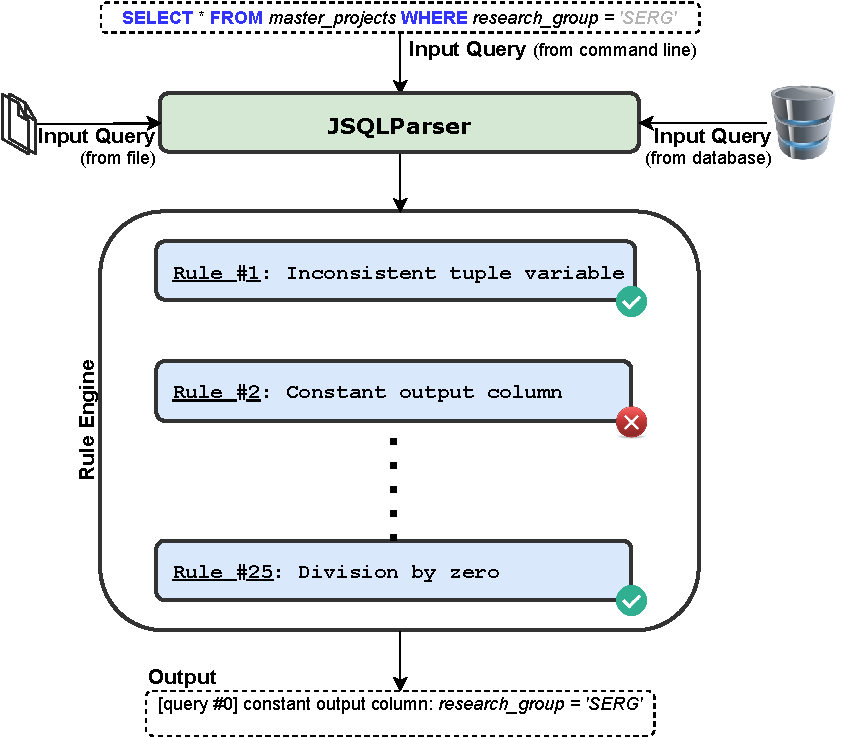
\includegraphics{img/tool_flow.pdf}
    \caption{Overall flow of the semantic bug detection tool}
    \label{fig:tool_flow}
\end{figure}

The detection strategies for each of the semantic bugs described in the previous sections are implemented as individual rules which make use of the visitor design pattern to parse SQL queries in search for different semantic bugs. Each rule focuses on detecting a single bug type. Furthermore, the tool is easily open for extension allowing for the implementation of numerous other rules for detecting other types of issues. Since for most rules there are a number of similarities such as parsing the queries in search for table sources or tuple variable names, there is a common interface shared by all the rules. 
One key aspect that we wanted to have for our tool was the ease of adding other rules in the future. In our current framework, this can easily be done by creating a new Java class and implementing the main interface which, among others, already takes care of parsing SQL queries. Developers then only have to override the methods for which custom functionality for the detection strategy is needed. This, for example, results in being able to write complicated heuristics for the rules without having to rewrite the parsing logic which saves both time as well as potential mistakes. Another important aspect is that rules can better be tested by only focusing on the new functionality which is specifically tailored for the detection strategy since the parsing logic is already tested by our framework.

The tool has three different modes of operation. In the first one, a query is entered via the command line and all the rules will be checked for finding semantic bugs in the input. This can be used whenever a fast check needs to be run for a single query in order to validate if this is semantically correct or not. The second mode of operation allows for an input file to be specified as input. The tool will then read all the queries from the file, which should be separated by a semicolon character (\sql{;}) and will display all the errors it detected for each of the SQL queries present in the file. This setting is perhaps more useful for conducting analysis on a larger input dataset. Finally, in the third mode of operation, the tool makes use of the Spring framework in order to connect to a MySQL database for retrieving input queries and running the rules on these. This mode was used during this research for analysing the large dataset of SQL queries collected from StackOverflow posts. The tool then also saves the results in this database which can later be used for further analysis.

Each rule is heavily covered by unit tests which try to account for general as well as more special edge cases. In total, there are more than 150 unit tests for the 25 rules implemented for our detection tool. Other tests include an automated script which uses a collection of more than 500 manually verified queries that runs against the tool and compares the outcome to the expected result. Some other 50 queries were manually checked in order to verify they do not contain any semantic errors after which they were presented as input to the tool in order to verify no warnings are raised, and later were added to the automated tests as well. The overall code quality for the tool was tracked on Better Code Hub, achieving an overall score of 9 out of 10 for quality, with the only area where maximum points were not scored being the separation of concerns in modules due to the shared interface used by all our rules. The source code for the tool together with all other scripts used for testing and analysing the results for this project can be found in GitHub at the following link: \url{https://github.com/cldme/SQLBugFinder}.


\section{Validation}
\label{section:validation}

Apart from the various unit tests implemented for checking each rule, the tool was validated using a manual process of investigating more than 500 SQL queries and verifying whether the output of the tool was correct or not. For each of the 25 semantic bug detection rules implemented in our tool, a random set of 20 queries collected from StackOverflow posts, for which the tool reported semantic bugs, was first selected in order to be manually analysed. The tool was configured such that each rule was run in isolation, meaning that every rule was analysed in detail, separately from the others, in order to confirm the correctness of both the implementation as well as the underlying heuristics used. Whenever a semantic bug was erroneously reported by the tool for a specific query, the code was analysed and fixed.

Furthermore, the unit tests were also improved to ensure the issues would not appear at a later stage when further modifications might be made to the rule. If multiple issues were found for a specific rule, after the initial set of 20 queries was verified, the process was restarted by selecting a new random set of 20 queries from the dataset for which the tool reported semantic bugs for the rule that was being checked. When no more errors were detected in the random sample, or none of the reported errors could be addressed, due to the fact that the query could not be parsed properly by the JSQLParser library or otherwise, the rule was considered to be sufficiently checked.
A dataset of roughly 500 queries was created, where for each rule the final set of 20 randomly selected queries together with the semantic bugs reported by the tool are registered. Furthermore, a script was implemented which uses this dataset together with the expected output to perform automated tests on the tool, in order to improve the testing of the rules.

\chapter{An Empirical Study on SQL Semantic Bugs in the Wild}
\label{chapter:semantic_bugs_study}

\section{Research methodology}
\label{section:research_methodology}

In this section we will present the research questions that this paper tries to answer. Furthermore, we also provide some more details regarding the datasets used in this research.

\begin{mdframed}
\noindent \textbf{RQ1:} \emph{What is the prevalence of semantic bugs in SQL queries?}
\end{mdframed}

With this research question, the aim is to investigate which are the most prevalent semantic bugs that appear in SQL queries. In order to analyse this, one of the most important aspects is being able to collect queries used in real world systems. For this, two datasets are used, one containing queries extracted from StackOverflow posts, and another dataset provided by \citet{P011} in their study on search-based test data generation for SQL queries. Both of these contain queries used in various open source projects and should provide a clear answer as to how often semantic bugs appear in SQL queries. To answer the question, we will run the rule-based static analysis tool designed for this project on all the collected queries and report on the total number of issues detected for each semantic bug. Furthermore, we also determine the median prevalence for each semantic bug as the ratio between the total number of queries having the semantic bug and the total number of collected queries in the dataset.

\begin{mdframed}
\noindent \textbf{RQ2:} \emph{What are the co-occurrences of semantic bugs in SQL queries?}
\end{mdframed}

The aim of this research question is to understand whether certain semantic bugs might tend to appear in pairs. It is valuable to know whether this is the case since if certain errors are detected in a query, then further attention can be paid to bugs that might co-occur. For answering this question, we use the results obtained for RQ1 from running the tool on all the collected queries, and then build a co-occurrence matrix for the semantic bugs. Furthermore, we also use the techniques described by \citet{P012} in order to compute the Jaccard index for normalizing co-occurrence data and present this in the form of a heat map. The Jaccard index is defined as the ratio between the number of times two bugs co-occur and the number of times for which at least one bug is observed to be present.

\begin{mdframed}
\noindent \textbf{RQ3:} \emph{What is the correlation between the complexity of a query and the number of semantic bugs it has?}
\end{mdframed}

Another interesting insight is knowing whether the complexity of a query has any correlation with the number of semantic bugs it has. By having this knowledge, whenever a query is detected as being too complex, this can already signal that potential semantic bugs might be present in the formulation of the query. In order to answer this question, we define and compute the complexity of a query as the total number of predicates, joins, subqueries, functions and columns it contains.

For analysing the correlation between the complexity of the query and the number of semantic bugs it has we will provide a box plot, which is the preferred visualization technique when dealing with both numerical and categorical data such as the one in our case, as described by \citet{P992} in their book on data visualization techniques. Furthermore we also provide the distribution for the query complexity scores. The data used in these visualizations will include our entire collection of SQL queries, from both the StackOverflow and the EvoSQL datasets.

Finally, we perform the one-way analysis of variance (ANOVA) test as described by \citet{P991} in order to determine whether or not there is a statistically significant difference between the means of our groups, which are given by the number of semantic bugs per query.

\section{Data collection}
\label{section:data_collection}
In this section we describe the approach used for building a large dataset of SQL queries collected from StackOverflow posts. StackOverflow is the main website where developers can ask questions and discuss various computer programming related issues which makes it one of the largest knowledge bases in this field. Apart from the 170,000 queries collected from StackOverflow, we also used for our study the dataset provided by \citet{P011} in their paper, which contains an additional 19,159 SQL queries extracted from various open source projects on GitHub.

The technique we used for extracting SQL queries from StackOverflow posts focused on retrieving the code block sections from each post and parsing these for finding valid SQL statements. For this, using an API for accessing the available StackOverflow data was preferred over other techniques such as web crawling since using an API is less intrusive for the StackOverflow platform. Google’s BigQuery public datasets now also include StackOverflow data, however these are not always up to date and further analysis showed these datasets are also not complete. In the end, for this paper, it was decided to use the Stack Exchange API\footnote{\url{https://api.stackexchange.com/}} which provides an interface for retrieving posts data from StackOverflow. Our query extraction tool only looks at SQL tagged questions, since these are the most likely to contain the queries we are interested in. Furthermore, before starting to process the posts, we filtered them on the number of votes they had, and sorted them in descending order, such that the more relevant and higher quality posts were processed first. In total, there are roughly 11,000 pages with SQL tagged questions on StackOverflow. For our study, we processed and extracted the queries from the top ranked 2000 pages. Our tool is capable of processing all pages, however we considered that enough queries were extracted to build a good dataset on which we could test our rule-based static analysis tool. Further studies could use the tool we developed in order to obtain an even larger dataset of queries should this be needed.

The Stack Exchange API offers functionality for creating a custom filter which is then included in the request providing fine control over the returned data. For our project, all metadata associated with a post was collected since the goal was building a complete dataset which might later be used for other research as well. Furthermore, it is important to point out that a distinction should be made between a question post and an answer post. A question post can have multiple answers associated with it and should also have at most one accepted answer. All posts, questions and answers, are created by one user, and have a score associated with them which indicates the number of upvotes a question or an answer has received. The intuition behind the score value for questions is that the higher the number, the more developers found that particular question useful, whereas for answers the higher the score the better the answer.

The collected data was organized in a MySQL database with four important schemas: owners, questions, answers and queries. In the owners table, the data about the user who created the post is stored together with any other metadata associated with the user. In the questions table, the data for the questions posts is stored and similarly in the answers table the data for all other posts is stored. Finally, in the queries table all extracted queries are saved together with an identifier which links the query to the post from which it was extracted. Since StackOverflow has no way of enforcing SQL syntax to be written in code block sections, this means that users are free to input any type of text inside the code blocks. Because of this, a special algorithm has to be used for extracting only the SQL statements from these sections.

Our approach for query extraction can be seen as an island parsing technique, similar to the solution proposed in \citet{P028}, where typically some recognizable structures are being parsed with detailed rules describing the constructs of interest, in our case the SQL keywords (the islands), and the remaining parts (the water), which in our case represent the overall query statement, are captured with other more generic rules. The algorithm used for extracting the queries from the code block section starts by first looking at every line and detecting whether it starts with a valid SQL keyword. If not, a number of additional checks are carried out in order to determine whether the line is part of an enumeration which was split on multiple rows. If this is still not the case, then the line is eliminated from the code block. After all lines from a code block section are parsed, all of them are collected into a single query. In case users input multiple SQL queries the algorithm also detects this by looking for the special semicolon character which indicates the end of an SQL statement. Another approach was also considered for the query extraction algorithm, which constructed the abstract syntax tree (AST) for each of the code blocks, however since these blocks might also contain non-SQL syntax as well, it was observed that more queries were extracted with the previous approach. Furthermore, another potential method could have been using a tool such as GitHub linguist\footnote{\url{https://github.com/github/linguist}} for automatically detecting the type of code present in the snippets and continue with further processing if SQL would have been detected. However, we did not explore this approach, but it might be something interesting to investigate in future studies on mining data from StackOverflow. Finally, all extracted queries are saved in the MySQL database and can later be processed by other tools such as SQL parsers like JSQLParser for determining whether the syntax of the query is indeed valid. We provide some descriptive statistics for the collected dataset in Table \ref{table:stackoverflow_stats}. The tool which extracts the queries is also made available on the GitHub page for our project at the following link: \url{https://github.com/cldme/SQLBugFinder/tree/main/queries_stack_exchange}

\begin{table}[ht]
\centering
\begin{tabular}{@{}lr@{}}
\toprule
\textbf{Statistic}                         & \textbf{Measurement} \\ \midrule
Total queries                              & 394,477         \\
Valid syntax                               & 172,232         \\
Invalid syntax                             & 22,2245         \\
Average response time for SQL questions    & 14m 54s        \\
Queries with semantic bugs                 & 28,386          \\
Queries with 1 semantic bug                & 24,229          \\
Queries with 2 semantic bugs               & 3572           \\
Queries with 3 semantic bugs               & 551            \\
Queries with 4 semantic bugs               & 32             \\
Queries with \textgreater{}5 semantic bugs & 2              \\ \bottomrule
\end{tabular}
\caption{General statistics for the StackOverflow dataset}
\label{table:stackoverflow_stats}
\end{table}

\section{Results}
\label{section:results}
In the following sections we discuss the results for each of the research questions and present our findings.

\subsection{RQ1: What is the prevalence of semantic bugs in SQL queries?}

We ran the rule-based static analysis tool containing 25 rules for detecting various SQL semantic bugs, as explained in Section \ref{section:detection_strategies}, on all collected queries. We observe that out of all 191,994 queries, a total of 36,818 queries which contain at least one semantic bug were identified, meaning that 19.17\% of queries contained some semantic problem in their formulation. Again, this shows the need for providing semantic bug detection tools for developers in order to improve the overall quality of SQL queries used in real world applications.

In Figure \ref{fig:prevalence} we show the prevalence of the detected semantic bugs in our StackOverflow dataset. Out of all these bugs, the most frequent one is the missing join predicates semantic bug (\sql{E019}), with a median prevalence of 5.98\%. The second most frequent semantic bug is the constant output column (\sql{E002}), which has a median prevalence of 3.62\% closely followed by the unnecessary count argument bug (\sql{E012}) with a median prevalence of 3.35\%. We did not detect any semantic bugs related to the use of identical tuple variables (\sql{E005}) in our collected dataset. For most of the other rules, the median prevalence was below 0.5\%, which means that out of 200 queries, one will be affected by a semantic bug.
We further analysed the rule for detecting missing join predicates by selecting 20 random queries for which this error was reported and manually checking the results of our tool. In all cases, we concluded that there were no false positive warnings and all errors were detected correctly. The same manual analysis was also conducted for all the other rules and we included the results in Appendix \ref{appendix:tool_validation}.

Other previous studies such as those conducted by \citet{P001} and \citet{P003} also concluded that the missing join predicates semantic bug is indeed frequent in SQL queries. One noticeable difference between previous study and our work comes from the datasets used. Most of the past work is based on queries collected from SQL courses, which means that queries are written by students on exams and other homework material. In our dataset, we used queries from various open source projects, hence the slightly lower median prevalence. Interestingly enough, \citet{P003} reports on 3.6\% prevalence for the constant output column semantic bug, again on a dataset of queries written by students on various exams, which is very close to the median prevalence we found in our study for the StackOverflow dataset, of 3.62\%.

In Figure \ref{fig:prevalence_evosql} we show the prevalence of the detected semantic bugs in the EvoSQL\footnote{\url{https://www.zenodo.org/record/1166023}} dataset. This dataset only contains SQL \sql{SELECT} queries found in three open source projects tracked on GitHub. Upon further manual inspection, it was observed that most of the queries suffered from the implicit columns SQL semantic code smell as described in the works of both \citet{P010} and \citet{P998}. In our implementation, this SQL semantic error corresponds to the constant output column bug (\sql{E002}), and as it can be observed from the results of our tool, this bug is indeed the most frequent one in the EvoSQL dataset with a median prevalence of 43.23\%. For all other semantic bugs, our tool detected a median prevalence of less than 0.4\% for this dataset.

\begin{mdframed}[default]
\noindent \textbf{RQ1 summary:} Out of all the collected queries, 19.17\% contained at least one semantic bug. The most common bugs are the missing join predicates (\sql{E019}) followed by the constant output column (\sql{E002}) and unnecessary count argument (\sql{E012}) bugs.
\end{mdframed}

\begin{figure}[ht]
    \centering
    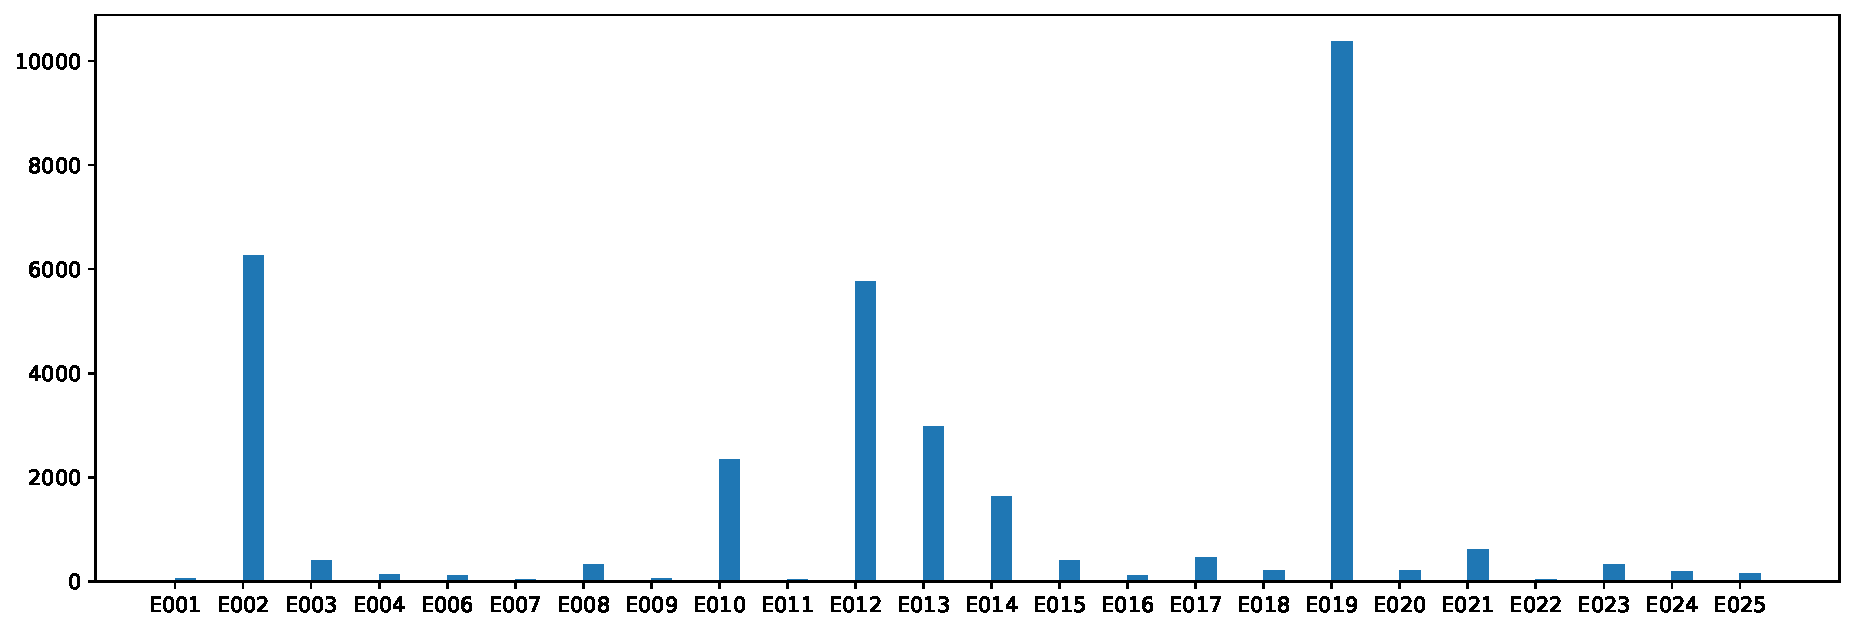
\includegraphics[width=1\textwidth]{img/prevalence.pdf}
    \caption{Prevalence of SQL semantic bugs for the StackOverflow dataset}
    \label{fig:prevalence}
\end{figure}

\begin{figure}[ht]
    \centering
    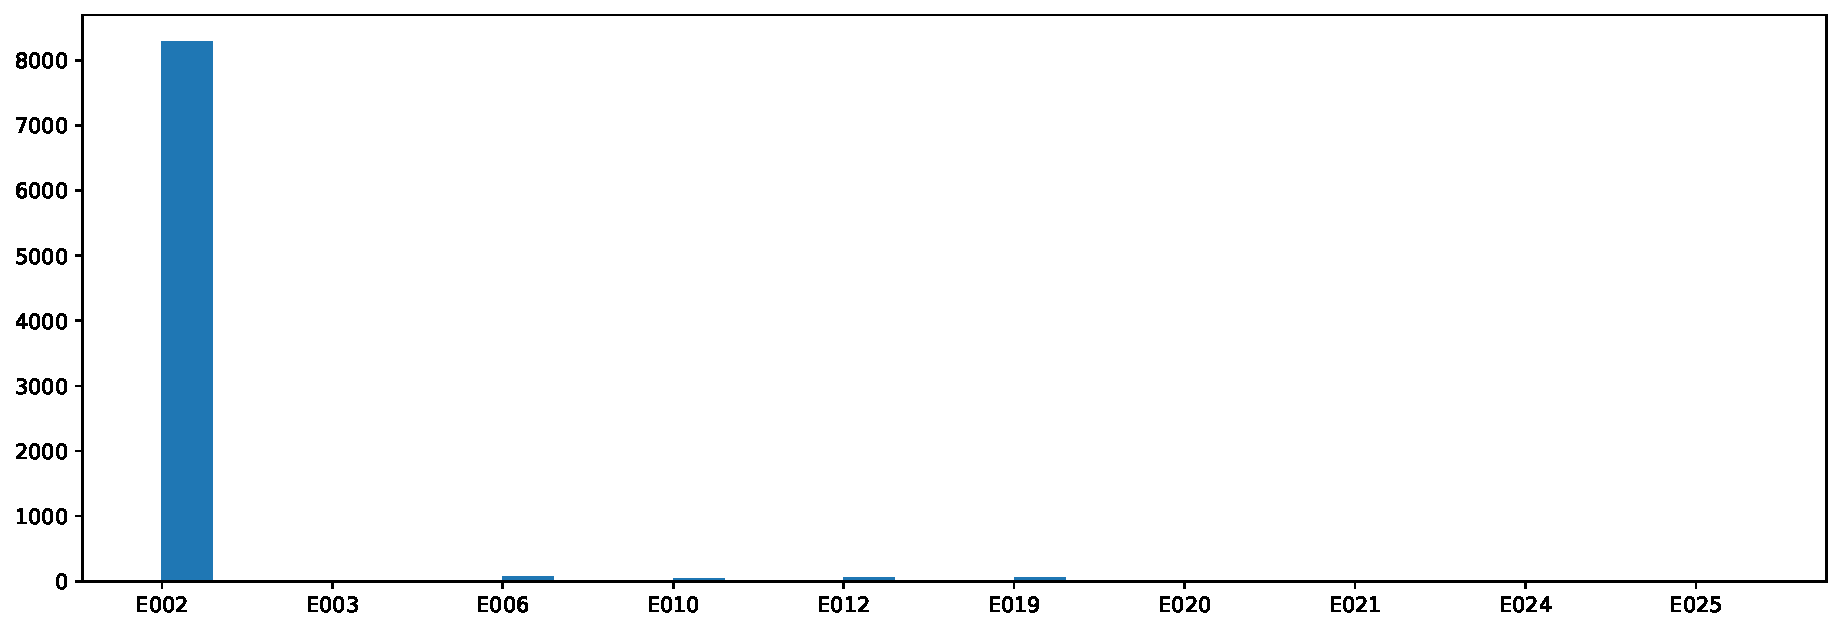
\includegraphics[width=1\textwidth]{img/prevalence_evosql.pdf}
    \caption{Prevalence of SQL semantic bugs for the EvoSQL dataset}
    \label{fig:prevalence_evosql}
\end{figure}

\subsection{RQ2: What are the co-occurrences of semantic bugs in SQL queries?}

In Figure \ref{fig:matrix} we show the co-occurrence matrix for our entire dataset, where each entry in the matrix represents the Jaccard similarity coefficient as described by \citet{P012} (empty cells have value zero). From this, we observe that most of the similarity values are rather low, however there is a 20\% similarity between bugs \sql{E012} and \sql{E013}, as well as a 15\% similarity between bugs \sql{E012} and \sql{E019}, followed by a 15\% similarity for bugs \sql{E002} and \sql{E019}. The Jaccard index is a measure of similarity between two sets of data, ranging from 0\% to 100\%, which means the higher the percentage, the more similar the two sets are to one another. In our case, for two bugs say A and B, if these have a 30\% similarity measure, this means that if bug A is detected in one query, then there is a 30\% probability that bug B is also present in this query.

This type of insight can be useful in designing future detection tools as well as prediction systems that could be integrated within IDEs in order to alert developers regarding certain bugs that their queries might contain given bugs which have already been detected. Further manual inspection for the queries where both the unnecessary count argument bug (\sql{E012}) as well as the unnecessary group by attribute error (\sql{E013}) both occur reveals that indeed these two types of semantic bugs are more likely to co-occur since usually the \sql{GROUP BY} clause is used with the intention of aggregating some data in the \sql{SELECT} clause.

Another interesting finding is that the missing join predicate bug (\sql{E019}) is the most likely one to co-occur with other types of bugs. More concretely, there is a 15\% similarity between queries containing bug \sql{E019} and either bug \sql{E002} or \sql{E012} and a 10\% similarity between queries containing bug \sql{E019} and either bug \sql{E013} or \sql{E015}. This also matches with the findings from \textbf{RQ1} which showed that bug \sql{E019} is the most prevalent one in our entire dataset, and as a result it co-occurs with 4 other different error types. 

\begin{mdframed}[default]
\noindent \textbf{RQ2 summary:} The co-occurrence of semantic bugs in SQL queries for our entire dataset is rather low, indicating that queries rarely contain more than one semantic bug. The highest similarity between two bugs is 20\%, for the unnecessary count argument (\sql{E012}) and unnecessary group by attribute (\sql{E013}).
\end{mdframed}

\begin{figure}[ht]
    \centering
    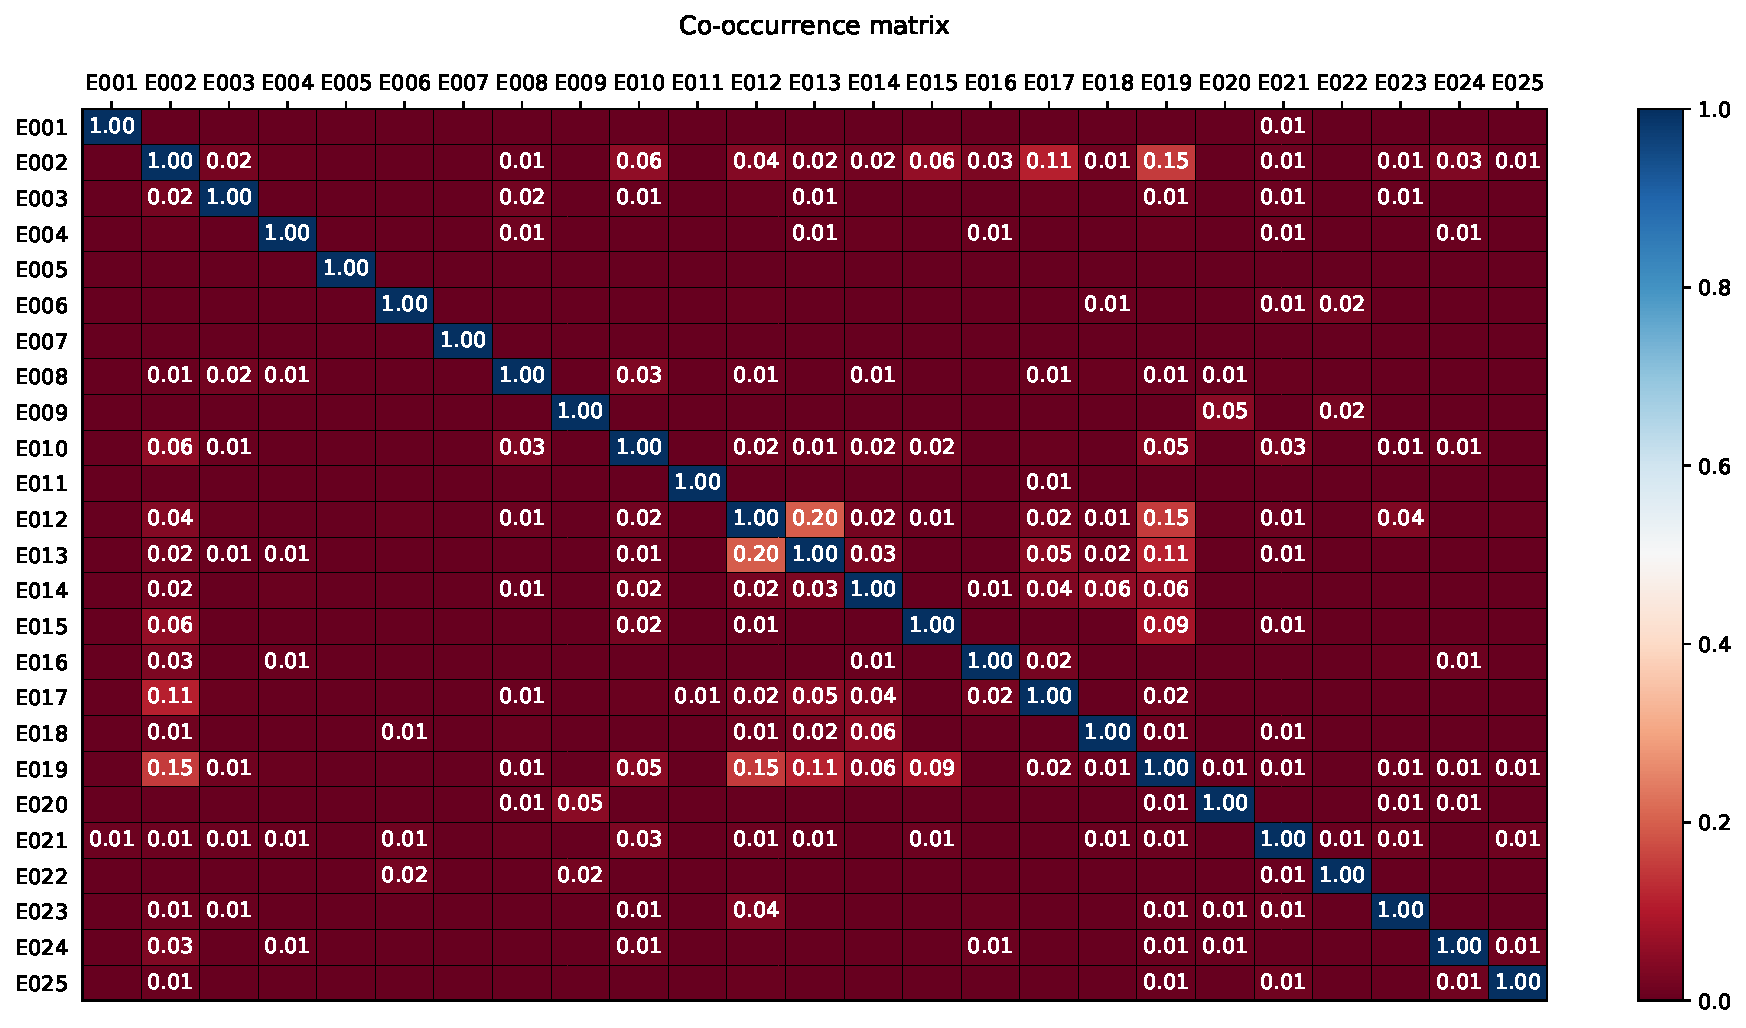
\includegraphics[width=1.1\textwidth]{img/matrix_combined.pdf}
    \caption{Co-occurrence matrix for SQL semantic bugs}
    \label{fig:matrix}
\end{figure}

\subsection{RQ3: What is the correlation between the complexity of a query and the number of semantic bugs it has?}

For analysing the correlation between the complexity of the query and the number of semantic bugs it has we provide a box plot in Figure \ref{fig:complexity_box}. In Figure \ref{fig:complexity_distribution} we also show the distribution of the query complexity scores. The data presented in these figures includes our entire collection of SQL queries, from both the StackOverflow and the EvoSQL datasets.

To further determine whether there is an correlation between the complexity of a query and the number of semantic bugs it has, we perform a one-way analysis of variance (ANOVA) test. For our one-way ANOVA test ($\alpha=0.05$) we define the following null and alternative hypotheses:

\begin{itemize}
    \item \textbf{$H_{0}$ (null hypothesis):} all the groups have the same mean, $\mu_{1} = \mu_{2} = \cdots = \mu_{5}$
    \item \textbf{$H_{1}$ (alternative hypothesis):} at least one of the means is different
\end{itemize}

We get that the corresponding p-value is $1.14$e-$168$, thus since this values is less our chosen $\alpha = 0.05$, we reject the null hypothesis, and can therefore say that there is significant difference between the considered groups. 

Computing the mean complexity score per category, we get that queries with a single semantic bug have a mean complexity of 7, queries with two bugs have a mean complexity of 10, queries with 3 bugs have mean complexity of 12, queries with 4 bugs have a mean complexity of 13 and finally queries with 5 bugs have a mean complexity of 26. 

\begin{mdframed}[default]
\noindent \textbf{RQ3 summary:} Performing an ANOVA test shows there is significant difference between the queries' complexities. There is also strong evidence which suggests that complex queries are more prone to suffer from SQL semantic bugs.
\end{mdframed}

\begin{figure}[ht]
    \centering
    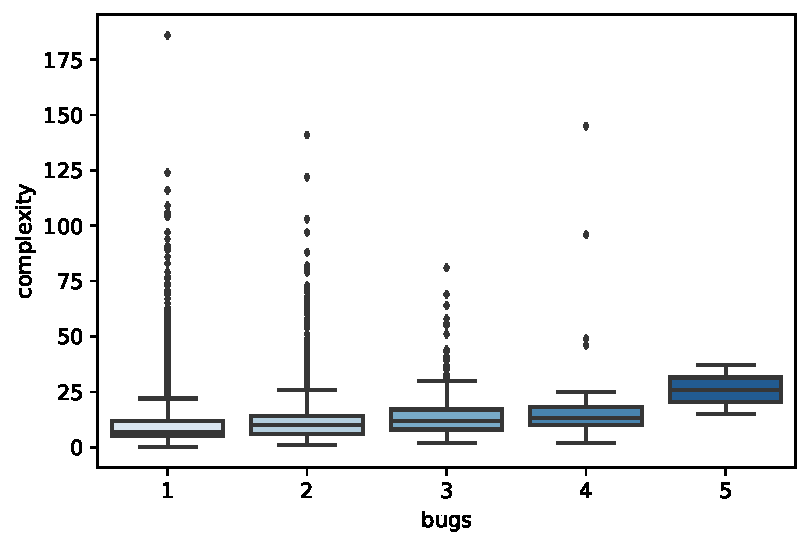
\includegraphics[width=0.7\textwidth]{img/complexity_box.pdf}
    \caption{Number of semantic bugs per query complexity}
    \label{fig:complexity_box}
\end{figure}

\begin{figure}[!htbp]
    \centering
    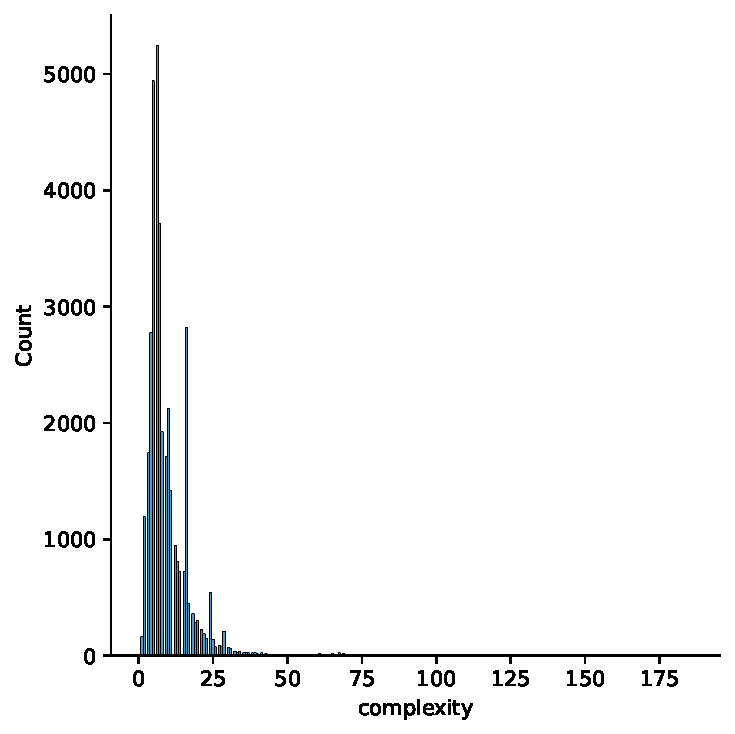
\includegraphics[width=0.7\textwidth]{img/complexity_distribution.pdf}
    \caption{Distribution of query complexity}
    \label{fig:complexity_distribution}
\end{figure}

\newpage
\section{Threats to validity}

In this section, we discuss the threats to the validity of this study and the actions we took to mitigate them.\\

\noindent \textbf{Internal validity.} The implementation of the heuristics for our rule-based static analysis tool can be subject to internal validity threats. To help with overcoming this, each of the 25 rules is covered by an extensive suite of unit tests, for both general as well as special edge case scenarios. Furthermore, we carried out a manual analysis of more than 500 queries, selecting for each of the 25 rules a random subset of 20 queries which were manually checked to ensure the results returned by the heuristics are correct. Finally, we also tried to align, as much as possible, the implementation of our heuristics, with the various implementation details found in previous research.\\

\noindent \textbf{External validity.} Although the collected dataset contains a diverse set of SQL queries, we observed that there are considerably more \sql{SELECT} queries than other types, such as \sql{INSERT}, \sql{UPDATE} or \sql{DELETE} queries, hence these latter types might be underrepresented in this study. This is especially noticeable in the EvoSQL dataset which only contains \sql{SELECT} queries. However, by extracting queries from StackOverflow posts, we hope to have overcome some of these issues, build a diverse enough collection of queries and at the same time have our results generalize on SQL queries in any software system.

\chapter{Conclusion}
\label{chapter:conclusion}

SQL is the most widely used database language, with more than 70\% of developers actively using it, as noted in a previous study \cite{P999}, however there is lacking support for detecting semantic issues, also known as code smells, in SQL queries. This is especially worrying seeing the high popularity of this language and its wide adoption in numerous industries, therefore the impact of potential problems with such queries can not be overstated.

Our goal with this thesis is two-fold. First, we propose a set of 25 validated heuristics for detecting the most common types of semantic bugs which appear in SQL queries, based on evidence from previous research. Second, we conduct an empirical study on the prevalence of semantic bugs in SQL using two datasets with queries extracted from three open-source projects as well as 190000+ queries collected from StackOverflow posts, building the largest collection of SQL queries to our knowledge. The correctness of the heuristics was manually verified from a random sample of more than 500 queries. 

We also provide a prototype implementation for a rule based static analysis tool, containing our 25 heuristics, for detecting semantic bugs. Our tool is able to detect semantic bugs in SQL queries with a 97\% accuracy. Furthermore, we observed that out of all the 191994 collected queries, 36818 contain at least one semantic bug, which means that 19.17\% of queries contained some semantic problem in their formulation. 

Analysing the prevalence of semantic bugs in SQL queries, we find that the most common bugs are missing join predicates (\sql{E019}) followed by the constant output column (\sql{E002}) and unnecessary count argument (\sql{E012}) bugs. We also found out that co-occurrence of semantic issues in SQL queries for our entire dataset is rather low, indicating that queries rarely contain more than one semantic bug. The highest similarity between two issues is 20\%, for the unnecessary count argument (\sql{E012}) and unnecessary group by attribute (\sql{E013}). 

Also quite interesting, we show that more complex queries, in terms of number of joins, predicates and functions used, tend to suffer from more semantic bugs, an interesting finding which could be used in the future as a metric for early prediction as to whether a query might contain semantic bugs or not.


\section{Recommendations}

In this section, we give some recommendations for developers, tool makers and researchers based on the findings made in our research.\\

\noindent \textbf{Recommendations for developers.} With so many applications relying on SQL for querying purposes, now more than ever it is crucial for developers to understand the implications of their queries suffering from various semantic issues. As we show in our empirical study, there are already quite a number of queries being shared online which already suffer from these types of problems, as it can be seen from Figure \ref{fig:prevalence}. Developers should therefore try to familiarize themselves not only with these semantic issues and how they appear when working with SQL, but they should also pay more attention to trying to detect these issues as well as address them as soon as they are discovered, just as bad code smells are addressed as well.\\

\noindent \textbf{Recommendations for tool makers.} The main focus here should be placed on designing tools for mass adoption. Choosing this as the main driving factor when building new tools should help with making sure that developers actually see value in the tool. More specifically, our findings show that it is currently hard for developers to check their SQL queries for semantic issues due to one underlying problem, which is the lack of adequate tools and support. Current implementations of tools that integrate with IDEs are lacking a lot when it comes to support for detecting semantic issues for queries, furthermore, there are also no tools, to our knowledge, which are integrated with popular development frameworks (such as SpringBoot) for checking these types of issues during application runtime. Especially interesting for future tools could be to integrate issue detection based on similarity measures, as we show in Figure \ref{fig:matrix} as well as early warnings based on metrics such as query complexity as we present in Figure \ref{fig:complexity_box}.\\

\noindent \textbf{Recommendations for researchers.} Based on the findings made when carrying out this study, we can say that current research places more focus on trying to develop techniques and methods for identifying syntactic issues in SQL queries. However, as we show in this paper and as well as other studies have pointed out, more emphasis should be placed on detecting semantic issues in queries as well. With implications ranging from performance issues to security vulnerabilities, having these types of semantic errors in any system is definitely detrimental. Therefore, it is quite crucial that in the near future, more research involving semantic issue detection for SQL will be carried out.


\section{Future work}

In this section we discuss the possible improvements that could be made to our detection tool as well as the query extraction algorithm and provide some ideas for future research which could make use of our large-scale SQL query dataset.

\begin{itemize}
    \item \textbf{Integrate the rule-based static analysis tool for detecting semantic issues in SQL queries into an IntelliJ/Eclipse plugin.} By providing support for our tool as an IDE plugin, developers can take advantage of it more easily. Other benefits could be real time detection of issues, when queries are written in the IDE as well as during runtime, when the application is executed, as an integration with the SpringBoot framework.
    \item \textbf{Improve the query extraction algorithm.} For retrieving queries from StackOverflow it would be interesting to investigate whether better results (more queries extracted) could be achieved by using a tool such as GitHub’s linguist\footnote{\url{https://github.com/github/linguist}} or Guesslang\footnote{\url{https://github.com/yoeo/guesslang}} for determining the programming language from within a code snippet.
    \item \textbf{Use our dataset to investigate whether developers notice SQL semantic issues in StackOverflow posts.} It would be interesting to analyse in future studies whether developers notice various types of semantic issues when either asking or replying to questions on StackOverflow. Another potential avenue for research could be to investigate the evolution of posts which might suffer from semantic issues in time and see if the problems are addressed.
    \item \textbf{Improve the rule-based static analysis tool by expanding the number of semantic issues which can be detected.} Although the tool is able to already detect the most common types of semantic issues which might occur in SQL queries, it would be very interesting to keep expanding this list by including other issues as well, such as the ones present in the closed source tool SQLEnlight. There is a comprehensive list\footnote{\url{https://sqlenlight.com/support/help/analysis-rules/}} with some of the semantic rules which this tool supports, so in the future one could port these into our detection tool as well.
\end{itemize}



\bibliographystyle{plainnat}
\bibliography{thesis}

\appendix
\def\chaptername{Appendix}
\chapter{Tool Validation}
\label{appendix:tool_validation}

For validating the correctness of the heuristics we implemented for our tool, a manual analysis of more than 500 queries was done. Each query was manually checked and the results returned by our tool were verified to detect, for each rule, how many of the reported warnings were valid. As presented in Section \ref{section:validation}, a random set of 20 queries was selected for each rule. We present the analysis below.

\begin{center}
\begingroup
\footnotesize
\begin{tabularx}{\linewidth}{ccXXc}
\toprule
\textbf{No.} & \textbf{RuleID} & \multicolumn{2}{X}{\textbf{Query}} & \textbf{Correct} \\ \midrule
1 & E001 & \multicolumn{2}{X}{\sql{select a1.owner,a1.table_name from all_tab_columns a1, all_tab_columns a2 where a1.owner=a2.owner and a1.table_name=a2.table_name and a1.column_name='location' and a2.column_name='asset_id' order by a1.owner,a1.table_name;}} & \emph{YES} \\ \hline
2 & E001 & \multicolumn{2}{X}{\sql{select t1.userid from userrole t1 join userrole t2 on t1.userid = t2.userid and t2.roleid = 2 join userrole t3 on t2.userid = t3.userid and t3.roleid = 3 and t1.roleid = 1;}} & \emph{YES} \\ \hline
3 & E001 & \multicolumn{2}{X}{\sql{select deptno from   dept where  exists(select * from   emp x where  x.deptno = 20 and exists(select * from   emp y where  y.job = x.job and y.deptno = dept.deptno)) and deptno <> 20;}} & \emph{YES} \\ \hline
4 & E001 & \multicolumn{2}{X}{\sql{select count(distinct patients.id) from public.patients, public.subscriptions, public.users, public.calendar_days where patients.user_id = users.id and patients.id = calendar_days.patient_id and subscriptions.user_id = patients.user_id and (date_trunc('day',patients.last_sync) > current_date - inter...}} & \emph{YES} \\ \hline
5 & E001 & \multicolumn{2}{X}{\sql{select * from tmp t0 where exists ( select * from tmp t1 join tmp t2 on t2.clientid = t1.clientid and t2.serverid = t1.serverid and t2.logtime > t1.logtime where t1. status = 'aborted' and t2. status = 'failed' and t1.clientid = t0.clientid and t1.serverid = t0.serverid and t1.logtime = t0.logtime o...}} & \emph{YES} \\ \hline
6 & E001 & \multicolumn{2}{X}{\sql{select distinct t.name from hospital_a t, hospital_a v where t.op_date=v.date_of_birth and t.surname=v.surname and t.op_id = 'p619920' and v.op_id = 'i552015';}} & \emph{NO} \\ \hline
7 & E001 & \multicolumn{2}{X}{\sql{select im1.imageid as id, im1.attributevalue as color, im2.attributevalue as quality from imageattribute im1, imageattribute im2 where im1.imageid = im2.imageid and im1.attributetype = "color" and im2.attributetype = "quality" and im2.attributevalue = "good";}} & \emph{YES} \\ \hline
8 & E001 & \multicolumn{2}{X}{\sql{select t1.a3 from test t1, test t2 where t1.a1 = t2.a1 and t2.a2 = t1.a2 and t1.a1 = t2.a2;}} & \emph{YES} \\ \hline
9 & E001 & \multicolumn{2}{X}{\sql{select * from audit a1 where not exists( select * from audit a2 where a2.status='approve' and a1.status='decline' and a2.id=a1.id );}} & \emph{YES} \\ \hline
10 & E001 & \multicolumn{2}{X}{\sql{select a.post_id, b.post_id, a.ul_value as "likes", b.ul_value as "dislikes" from wp_like_dislike_counters as a, wp_like_dislike_counters as b where a.post_id = b.post_id and a.ul_key = 'u_like' and b.ul_key = 'u_dislike';}} & \emph{NO} \\ \hline
11 & E001 & \multicolumn{2}{X}{\sql{update users set online = 1 where exists(select null from users t where t.email = in_email and t.password = in_password and t.id = id) and id = 'result_id';}} & \emph{YES} \\ \hline
12 & E001 & \multicolumn{2}{X}{\sql{select p1.domain_id, p2.domain_id, count(p1.domain_id) as d1, count(p2.domain_id) as d2 from pdb as p1, interacting_pdbs as i1, pdb as p2, interacting_pdbs as i2 where p1.id = i1.pdb_first_id and p2.id = i2.pdb_second_id and i1.id = i2.id group by p1.domain_id, p2.domain_id having d1 > 100 and d2 > ...}} & \emph{YES} \\ \hline
13 & E001 & \multicolumn{2}{X}{\sql{select a.object from mytable a, mytable b where a.object = b.object and a.key = 'a' and a.value = 'a' and b.key = 'b' and b.value = 'b';}} & \emph{YES} \\ \hline
14 & E001 & \multicolumn{2}{X}{\sql{select * from cats outside where not exists(select * from cats cat where exists( select dog.foo,dog.bar from dogs dog where cat.foo = dog.foo and cat.bar = dog.bar) and outside.foo = cat.foo and outside.bar=cat.bar );}} & \emph{YES} \\ \hline
15 & E001 & \multicolumn{2}{X}{\sql{select username.name, useremail.email, userphone.phone from users as username inner join users as useremail on username.user = useremail.user and username.field = 'name' and useremail.field = 'email' inner join users as userphone on username.user = userphone.user and userphone.field = 'phone';}} & \emph{NO} \\ \hline
16 & E001 & \multicolumn{2}{X}{\sql{select count(*) from ( select u1.userid from vote u1, vote u2 where u1.itemid = u2.itemid and u1.userid = user1 and u2.userid = user2);}} & \emph{YES} \\ \hline
17 & E001 & \multicolumn{2}{X}{\sql{update mark set mark= case when mark.val<= 5 then val*1.1 else val end where mark.id_classes = classes.id_classes and classes.id_subject = subject.id_subject and subject.id_subject = 5;}} & \emph{YES} \\ \hline
18 & E001 & \multicolumn{2}{X}{\sql{select a1.owner,a1.table_name from all_tab_columns a1, all_tab_columns a2 where a1.owner=a2.owner and a1.table_name=a2.table_name and a1.column_name='location' and a2.column_name='asset_id' order by a1.owner,a1.table_name;}} & \emph{YES} \\ \hline
19 & E001 & \multicolumn{2}{X}{\sql{select p1.gameid from participants as p1, participants as p2 where p1.name = 'team1' and p2.name='team2' and p1.gameid = p2.gameid;}} & \emph{NO} \\ \hline
20 & E001 & \multicolumn{2}{X}{\sql{select n1.id, n1.name,n2.name, a3.age from name n1, name n2, age a3 where n1.id=n2.id and n1.id=a3.id and n1.type=0   and n2.type=1;}} & \emph{YES} \\ \hline
\caption{Manual analysis of tool performance for rule E001}
\end{tabularx}
\endgroup
\end{center}


\begin{center}
\begingroup
\footnotesize
\begin{tabularx}{\linewidth}{ccXXc}
\toprule
\textbf{No.} & \textbf{RuleID} & \multicolumn{2}{X}{\textbf{Query}} & \textbf{Correct} \\ \midrule
21 & E002 & \multicolumn{2}{X}{\sql{select * from mytable1 ca left outer join mytable2 dcn on dcn.dstrct_code = ca.dstrct_code where ca.dstrct_code = '0001' and ca.req_232_type = 'p' and ca.requisition_no = '264982  000' and ca.alloc_count = '01' order by ca.alloc_count asc;}} & \emph{YES} \\ \hline
22 & E002 & \multicolumn{2}{X}{\sql{select * from ranked where ranking = 1;}} & \emph{YES} \\ \hline
23 & E002 & \multicolumn{2}{X}{\sql{select * from orc_users as  t1 inner join orc_files as t2 on t1.id = t2.userid where t1.email='sdfsdf';}} & \emph{YES} \\ \hline
24 & E002 & \multicolumn{2}{X}{\sql{select * from person where name = 'robert';}} & \emph{YES} \\ \hline
25 & E002 & \multicolumn{2}{X}{\sql{select * from myuser as u join friend_pivotal as p on u.id = p.user_rec_id or u.id = p.user_inv_id where status = 'accepted';}} & \emph{YES} \\ \hline
26 & E002 & \multicolumn{2}{X}{\sql{select * from (select * from table order by value desc, date_column) where rownum = 1;}} & \emph{YES} \\ \hline
27 & E002 & \multicolumn{2}{X}{\sql{select * from a_table where a_column = '&avariable' union select * from a_table where b_column = '&&avariable';}} & \emph{YES} \\ \hline
28 & E002 & \multicolumn{2}{X}{\sql{select incurredcharges.procedure_no, incurredcharges.patient_no, charges.procedure from incurredcharges inner join charges where incurredcharges.patient_no=12;}} & \emph{YES} \\ \hline
29 & E002 & \multicolumn{2}{X}{\sql{select u.uid ,u.uname,p.uid , p.profname,e.uid,e.eduname from  user  u inner join profession p on u.uid=p.pid inner join education e on u.uid = e.uid where u.uid=p.uid and u.uid=e.uid and i.uid=1;}} & \emph{YES} \\ \hline
30 & E002 & \multicolumn{2}{X}{\sql{select arbogast.node.nid as anid, mcguffin.node.nid as mnid, arbogast.node.title as atitle, mcguffin.node.title as mtitle from arbogast.node, mcguffin.node where arbogast.node.nid = 1 and mcguffin.node.nid = arbogast.node.nid;}} & \emph{YES} \\ \hline
31 & E002 & \multicolumn{2}{X}{\sql{select imagename, sum(ratingvalue) as "lol" from ratings group by imagename having imagename = 'myimagename';}} & \emph{YES} \\ \hline
32 & E002 & \multicolumn{2}{X}{\sql{select max(id) as id, type, max(other_id) as other_id, max(def_id) as def_id, ref_def_id from t where type = 'ref' group by type, ref_def_id;}} & \emph{YES} \\ \hline
33 & E002 & \multicolumn{2}{X}{\sql{select distinct name from sys.objects where type in ('u','v') and name= 'myname';}} & \emph{YES} \\ \hline
34 & E002 & \multicolumn{2}{X}{\sql{select customerid, orderdate, count(1) cnt from sales.salesorderheader where customerid = 11300 group by customerid, orderdate order by cnt desc;}} & \emph{YES} \\ \hline
35 & E002 & \multicolumn{2}{X}{\sql{select booking.bookno, booking.courno, course.coursename from booking, course, coursename where booking.bookno = 6200 and booking.courno = course.courno and coursename.coursenameno = course.coursenameno;}} & \emph{YES} \\ \hline
36 & E002 & \multicolumn{2}{X}{\sql{select table1.personcode, table1.name, table2.location, max(table2.servicedate) from table1 inner join table2 on table1.id = table2.table1id where table1.personcode = 'xyz' group by table1.personcode,table1.name, table2.location;}} & \emph{YES} \\ \hline
37 & E002 & \multicolumn{2}{X}{\sql{select t1.userid, t2.date, min(t1.time) as in_time, max(t1.time) as out_time from test t1 join (select distinct date from test where userid = 609) t2 where t1.date = t2.date and userid = 609 group by t1.userid, t2.date;}} & \emph{YES} \\ \hline
38 & E002 & \multicolumn{2}{X}{\sql{select * from mm_tfs where product_description like '\%football\%' and schoolid = '8' and category_id ='21';}} & \emph{YES} \\ \hline
39 & E002 & \multicolumn{2}{X}{\sql{select * from customer where c_role = 'dev' order by c_id limit 2;}} & \emph{YES} \\ \hline
40 & E002 & \multicolumn{2}{X}{\sql{select attrsmall, attrlarge, max(rating_id) as ratingmax from ( select case when c.attr1_id < c.attr2_id then c.attr1_id else c.attr2_id end as attrsmall, case when c.attr1_id < c.attr2_id then c.attr2_id else c.attr1_id end as attrlarge, c.rating_id from compatibility c) as c1 group by atrrsmall, a...}} & \emph{YES} \\ \hline
\caption{Manual analysis of tool performance for rule E002}
\end{tabularx}
\endgroup
\end{center}


\begin{center}
\begingroup
\footnotesize
\begin{tabularx}{\linewidth}{ccXXc}
\toprule
\textbf{No.} & \textbf{RuleID} & \multicolumn{2}{X}{\textbf{Query}} & \textbf{Correct} \\ \midrule
41 & E003 & \multicolumn{2}{X}{\sql{insert into personpet(fk_person, fk_pet) select id, id from person;}} & \emph{YES} \\ \hline
42 & E003 & \multicolumn{2}{X}{\sql{select identity( int ) as tempid, *, sectionid as fix2ids from files_sections;}} & \emph{YES} \\ \hline
43 & E003 & \multicolumn{2}{X}{\sql{select *, cond2 as cond2, cond3 as cond3 from table having cond1 and (cond2 or cond3);}} & \emph{YES} \\ \hline
44 & E003 & \multicolumn{2}{X}{\sql{select country, count(*) as cnt1, count(*) as cnt2 from orders group by country having cnt1=2 and cnt2>2;}} & \emph{YES} \\ \hline
45 & E003 & \multicolumn{2}{X}{\sql{select c77,c77,c125,c126,c127,c74 from mytable;}} & \emph{YES} \\ \hline
46 & E003 & \multicolumn{2}{X}{\sql{select itemnumber as '@id', itemnumber as 'itemnumber', price as 'price/@value', datefrom as 'price/datefrom', dateto as 'price/dateto' from \#tempxml;}} & \emph{YES} \\ \hline
47 & E003 & \multicolumn{2}{X}{\sql{select videos.id, videos.id as video_id, videos.video_title as video_title, group_concat(distinct t.tag_name separator '|') as tag_names from   videos join   video_tags as vt join   tags as t where  videos.id <= ( select  max_doc_id from    sph_counter where   counter_id = 1 ) group by videos.id;}} & \emph{YES} \\ \hline
48 & E003 & \multicolumn{2}{X}{\sql{select distinct t.date_effective, t.acct_account_transaction_id, p.method, t.amount, c.business_name, t.amount from   contact                  c join   contact_role            cr on cr.contact_fk = c.contact_id join   acct_account             a on a.contact_fk = c.contact_id join   acct_account_tran...}} & \emph{YES} \\ \hline
49 & E003 & \multicolumn{2}{X}{\sql{insert into test_table(column_1, column_2) select val, val from x;}} & \emph{YES} \\ \hline
50 & E003 & \multicolumn{2}{X}{\sql{select e.empid,e.fname,e.lname,c.description as hair,c.description as race from employee2 e  inner join code c;}} & \emph{YES} \\ \hline
51 & E003 & \multicolumn{2}{X}{\sql{select uuid, uuid from data;}} & \emph{YES} \\ \hline
52 & E003 & \multicolumn{2}{X}{\sql{select value, value from public.customers where nodevalue.key3 = 'key3' and nodevalue.key4 = 'key4';}} & \emph{YES} \\ \hline
53 & E003 & \multicolumn{2}{X}{\sql{select owner, count(distinct object_name || 'this is a really long string in my expression, don''t you think?  actually, it''s really, really, really, really, really, really, really, really, really, really, really, really, really, really, really, really, really, really, really, really, really, reall...}} & \emph{YES} \\ \hline
54 & E003 & \multicolumn{2}{X}{\sql{select projects.project_id, projects.title, projects.start_time, projects.description, projects.user_id, projects.winner_user_id, users.username as owner, users.username as winner from projects,users where projects.user_id=users.user_id and projects.winner_user_id=users.user_id;}} & \emph{YES} \\ \hline
55 & E003 & \multicolumn{2}{X}{\sql{select productgroupid as product23_1_, articleid as articleid1_, articleid as articleid18_0_, inventory_name as inventory3_18_0_, inventory_unitofmeasure as inventory4_18_0_, businesskey as business5_18_0_, name as name18_0_, servespeople as servespe7_18_0_, instock as instock18_0_, description as d...}} & \emph{YES} \\ \hline
56 & E003 & \multicolumn{2}{X}{\sql{select *, t1.image_id as  image from event.dbo.dia_tracker t1 where exists (select 1 from event.dbo.dia_tracker t2 where t2.patient_id = 'dsma' group by case when t2.active = '1' then t2.image_id end having max(t2.image_id ) = t1.image_id);}} & \emph{YES} \\ \hline
57 & E003 & \multicolumn{2}{X}{\sql{select *, 'full' from abc;}} & \emph{YES} \\ \hline
58 & E003 & \multicolumn{2}{X}{\sql{select 1 except select 1;}} & \emph{NO} \\ \hline
59 & E003 & \multicolumn{2}{X}{\sql{select *, regexp_replace(port, '[0-9/\.]', '', 'g') port_name, string_to_array(regexp_replace(port, '[a-za-z\-]', '', 'g'), '/')::float[] port_number from device order by name, regexp_replace(port, '[0-9/\.]', '', 'g'), string_to_array(regexp_replace(port, '[a-za-z\-]', '', 'g'), '/')::float[];}} & \emph{YES} \\ \hline
60 & E003 & \multicolumn{2}{X}{\sql{select *, match(pages) against('doodle') as score from books where match(pages) against('doodle') order by score desc;}} & \emph{YES} \\ \hline
\caption{Manual analysis of tool performance for rule E003}
\end{tabularx}
\endgroup
\end{center}


\begin{center}
\begingroup
\footnotesize
\begin{tabularx}{\linewidth}{ccXXc}
\toprule
\textbf{No.} & \textbf{RuleID} & \multicolumn{2}{X}{\textbf{Query}} & \textbf{Correct} \\ \midrule
61 & E004 & \multicolumn{2}{X}{\sql{select emp.salary from employee emp inner join sap s on emp.id = s.id where s.id = 111;}} & \emph{YES} \\ \hline
62 & E004 & \multicolumn{2}{X}{\sql{select * from child c,parent p where c.id=p.parentid and c.parentid !=0;}} & \emph{YES} \\ \hline
63 & E004 & \multicolumn{2}{X}{\sql{select t1.col_1 from table t1 join table t2 on t1.col_2=t2.col_1 where t1.col_1=t2.col_2 and t1.col_1='one';}} & \emph{YES} \\ \hline
64 & E004 & \multicolumn{2}{X}{\sql{select m.actor from movies m where m.movie = 'pulp fiction' and not exists ( select 1 from movies m1 join movies m2 on m1.movie = m2.movie and m1.actor <> m2.actor and m2.movie <> 'pulp fiction' and m2.actor in (select actor from movies where movie = 'pulp fiction') where m.actor = m1.actor );}} & \emph{YES} \\ \hline
65 & E004 & \multicolumn{2}{X}{\sql{select c.name, if(find_in_set('type_a', group_concat(substring_index(f1.filename,'_',2))), 'yes', 'no') as type_a, if(find_in_set('type_b', group_concat(substring_index(f1.filename,'_',2))), 'yes', 'no') as type_b, if(find_in_set('type_c', group_concat(substring_index(f1.filename,'_',2))), 'yes', 'n...}} & \emph{YES} \\ \hline
66 & E004 & \multicolumn{2}{X}{\sql{select u.firstname, u.lastname, u.rep, u.email, u.password, u.gender, u.level, u.birthday, u.achievements, u.height, u.unit, u.cityid, u.countryid, r.regdate, ci.name as city, co.name as country from users u, registry r, cities ci, countries co where u.id = 1 and r.uid = u.id and u.cityid = ci.id an...}} & \emph{YES} \\ \hline
67 & E004 & \multicolumn{2}{X}{\sql{select images.*, users.username from images left join users on images.user_id = users.id left join user_follow on images.user_id = user_follow.follow_id where images.user_id = 3 or user_follow.user_id = 3 order by images.date desc;}} & \emph{YES} \\ \hline
68 & E004 & \multicolumn{2}{X}{\sql{select * from tblpe t1 where t1.date = ( select max(date) from tblpe t2 where t1.id = t2.id ) and t1.id = 39;}} & \emph{YES} \\ \hline
69 & E004 & \multicolumn{2}{X}{\sql{select pd.id,pd.price_date,pd.name_id,pd.class_id,pd.currency_id,pd.price, pd.price - (select price from price_data as x where x.price_date < pd.price_date and x.name_id      = pd.name_id and x.class_id     = pd.class_id and x.currency_id  = pd.currency_id having max(x.price_date)) as `change` from ...}} & \emph{YES} \\ \hline
70 & E004 & \multicolumn{2}{X}{\sql{select activitytext, actiontext from activity join activityaction on activity.activityid = activityaction.activityid join action on activityaction.actionid = action.actionid where activity.activityid = 1;}} & \emph{YES} \\ \hline
71 & E004 & \multicolumn{2}{X}{\sql{select studentid, firstname, lastname, gender from   student join major on student.majorid = major.majorid where  major.majorid = 2;}} & \emph{YES} \\ \hline
72 & E004 & \multicolumn{2}{X}{\sql{select col.column_name, col.constraint_name from information_schema.constraint_column_usage col where col.constraint_name = tab.constraint_name and col.table_name = tab.table_name and constraint_type = 'primary key' and col.constraint_name like '\%adhoc\%';}} & \emph{YES} \\ \hline
73 & E004 & \multicolumn{2}{X}{\sql{update purchase as p inner join artwork as a on p.purchaseid = a.purchaseid set p.total = sum(a.price) where a.purchaseid = 'd4758';}} & \emph{YES} \\ \hline
74 & E004 & \multicolumn{2}{X}{\sql{select client.*, cat1id.client_catid_1 as cat1, cat2id.client_catid_2 as cat2 from tb_clients as client left join tb_clients_categories cat1id on client.client_id = cat1id.client_id left join tb_clients_categories cat2id on client.client_id = cat2id.client_id where client.client_id = 65447;}} & \emph{YES} \\ \hline
75 & E004 & \multicolumn{2}{X}{\sql{select c.c_id, s.s_fname, count(r.c_id) from results r, candidates c, student s,positioning p, organization o where r.c_id = c.c_id and c.sid = s.sid and c.pos_id = p.pos_id and o.org_id = c.org_id and o.org_id = 1 group by c.c_id;}} & \emph{YES} \\ \hline
76 & E004 & \multicolumn{2}{X}{\sql{select pt.projecttaskid, isnull(sum(case when pte.assigneduserid = @userid then 1 end),0) as assignedtome, isnull(sum(case when pte.assigneduserid <> @userid then 1 end),0) as assignedtoothers from projecttask pt inner join project p on p.projectid = pt.projectid left join projecttaskentity pte on p...}} & \emph{YES} \\ \hline
77 & E004 & \multicolumn{2}{X}{\sql{select ip_settings.ip from server inner join network_interfaces on network_interfaces.id = server.fk_network_interfaces inner join ip_settings on ip_settings.id = network_interfaces.fk_ip_settings where server.id=6;}} & \emph{YES} \\ \hline
78 & E004 & \multicolumn{2}{X}{\sql{update table_to tt, table_from tf set tt.name = "chandi" where tt.id = tf.id and tf.id = 1;}} & \emph{YES} \\ \hline
79 & E004 & \multicolumn{2}{X}{\sql{select t.* from terms t join term_relationships tr on tr.term_id = t.term_id join posts p on p.post_id = tr.post_id where p.post_id = 1;}} & \emph{YES} \\ \hline
80 & E004 & \multicolumn{2}{X}{\sql{select t1.service from table1 t1, table2 t2 where t1.cnty = t2.cnty and t1.zip = t2.zip and t2.zip = '1234';}} & \emph{YES} \\ \hline
\caption{Manual analysis of tool performance for rule E004}
\end{tabularx}
\endgroup
\end{center}


\begin{center}
\begingroup
\footnotesize
\begin{tabularx}{\linewidth}{ccXXc}
\toprule
\textbf{No.} & \textbf{RuleID} & \multicolumn{2}{X}{\textbf{Query}} & \textbf{Correct} \\ \midrule
81 & E006 & \multicolumn{2}{X}{\sql{select * from (values (1), (2)) as tbl(col) where not (col = null or col = 1);}} & \emph{YES} \\ \hline
82 & E006 & \multicolumn{2}{X}{\sql{select r.id, r.authtoken.instagram,r.username from root r where r.abc <> null;}} & \emph{YES} \\ \hline
83 & E006 & \multicolumn{2}{X}{\sql{select loans.*, if(ul.name = null, ub.name, ul.name) as name, if(ul.id = null, ub.id,ul.id) as uid from loans left join users ul on users.id = loans.lender_id left join users ub on users.id = loans.borrower_id where ul.id = 2 or ub.id = 2;}} & \emph{YES} \\ \hline
84 & E006 & \multicolumn{2}{X}{\sql{select count(*) from table1 where request_time < timestamp'2012-05-19 14:00:00' and (end_time > timestamp'2012-05-19 14:00:00' or end_time=null);}} & \emph{YES} \\ \hline
85 & E006 & \multicolumn{2}{X}{\sql{select * from my_table where some_field = null;}} & \emph{YES} \\ \hline
86 & E006 & \multicolumn{2}{X}{\sql{select * from customer c where so.orderid = null;}} & \emph{YES} \\ \hline
87 & E006 & \multicolumn{2}{X}{\sql{select name from bbc where gdp > all (select gdp from bbc where region = 'africa' and gdp<>null);}} & \emph{YES} \\ \hline
88 & E006 & \multicolumn{2}{X}{\sql{select * from hotel where address != null;}} & \emph{YES} \\ \hline
89 & E006 & \multicolumn{2}{X}{\sql{select * from t1 where a=b or (a=null and b=null);}} & \emph{YES} \\ \hline
90 & E006 & \multicolumn{2}{X}{\sql{select concat(area, yearlevel, code) as subjectcode, count(student) from studenttakessubject where result < 50 and result <> null group by code having count(student) > 1;}} & \emph{YES} \\ \hline
91 & E006 & \multicolumn{2}{X}{\sql{select checklists.id from checklists left join (select checklist_id from checklist_items where completed = 'f' union distinct select checklist_id from checklist_items group by checklist_id having count(*) = 0) partial_checklists where partial_checklists.checklist_id = null;}} & \emph{YES} \\ \hline
92 & E006 & \multicolumn{2}{X}{\sql{select lefttable.id, righttable.id as nullid from lefttable left join righttable on righttable.id = lefttable.id where nullid = null;}} & \emph{YES} \\ \hline
93 & E006 & \multicolumn{2}{X}{\sql{select e.id from employments e where not exists ( select 1 from emails em where em.employment_id=e.id and em.deactivated_on = null );}} & \emph{YES} \\ \hline
94 & E006 & \multicolumn{2}{X}{\sql{select secid, min(date) as startdate, max(date) as enddate, price from bigtable group by secid, enddate having min(date) != max(date) and date != null;}} & \emph{YES} \\ \hline
95 & E006 & \multicolumn{2}{X}{\sql{select * from student left join course where student.std_id = null or student.std_name = null or student.std_start_date = null or student.std_end_date = null or student.std_gender = null or student.course_id = null;}} & \emph{YES} \\ \hline
96 & E006 & \multicolumn{2}{X}{\sql{select top (10) ctry, sales from table1 union all select 'other', sum(sales) from table1 where table2.ctry = null group by table1.ctry;}} & \emph{YES} \\ \hline
97 & E006 & \multicolumn{2}{X}{\sql{update salesorders o set transref = (select t.transref from transfers t where o.orderno = t.orderno and (o.ordext = t.ordext or (t.ordext=null and o.ordext=null)) and t.transref <> null) where ordext = null;}} & \emph{YES} \\ \hline
98 & E006 & \multicolumn{2}{X}{\sql{select h.clientnumber, iif(h.checkoutdate=null,"yes","") as currentvisitor from visitstable as h inner join ( select clientnumber, max(lastvisitdate) as lastvisitstart from visitstable group by clientnumber) as t;}} & \emph{YES} \\ \hline
99 & E006 & \multicolumn{2}{X}{\sql{select * from t left join m on t.sub_id = m.id where t.sub_id != null;}} & \emph{YES} \\ \hline
100 & E006 & \multicolumn{2}{X}{\sql{select m.provider_id, m.provider_name, p.purchase_order_code, null as purchase_order_sample_code, p.provider_id as provider_order from mst_provider as m left join trx_purchase_order as p where p.provider_id != null union select m.provider_id, m.provider_name, p.purchase_order_code, null as purchase_...}} & \emph{YES} \\ \hline
\caption{Manual analysis of tool performance for rule E006}
\end{tabularx}
\endgroup
\end{center}


\begin{center}
\begingroup
\footnotesize
\begin{tabularx}{\linewidth}{ccXXc}
\toprule
\textbf{No.} & \textbf{RuleID} & \multicolumn{2}{X}{\textbf{Query}} & \textbf{Correct} \\ \midrule
101 & E007 & \multicolumn{2}{X}{\sql{select sum(amt) where session=x and order >= ( select max(order) where atype='set' and session=x );}} & \emph{YES} \\ \hline
102 & E007 & \multicolumn{2}{X}{\sql{select t.*, row_number() over(partition by "name" order by "date") as rank from  tablea t where "date" >= (select max("date") from tablea where "type" = 'b');}} & \emph{YES} \\ \hline
103 & E007 & \multicolumn{2}{X}{\sql{select * from `table_name` where id >= (select floor( max(id) * rand()) from `table_name` ) order by id limit 30;}} & \emph{YES} \\ \hline
104 & E007 & \multicolumn{2}{X}{\sql{select id from table_name where id >= (select max(id) from table_name where id <= 12);}} & \emph{YES} \\ \hline
105 & E007 & \multicolumn{2}{X}{\sql{select thedate from datetable where thedate >= (select max(thedate) from datetable where thedate < getdate());}} & \emph{YES} \\ \hline
106 & E007 & \multicolumn{2}{X}{\sql{select distinct maker, price from product inner join printer where color = 'y' and price <= (select min(price) from printer where color = 'y');}} & \emph{YES} \\ \hline
107 & E007 & \multicolumn{2}{X}{\sql{select * from numbers where nr >= (select max(nr) from numbers where nr < 6.20) and nr <= (select min(nr) from numbers where nr > 6.20);}} & \emph{YES} \\ \hline
108 & E007 & \multicolumn{2}{X}{\sql{select name, message from flux_chat_messages where id >= ( max( id ) -5 ) order by id asc;}} & \emph{YES} \\ \hline
109 & E007 & \multicolumn{2}{X}{\sql{select submissionid, input, value from yourtable where submissionid >= (select max(submissionid) from yourtable) - 1 order by submissionid;}} & \emph{YES} \\ \hline
110 & E007 & \multicolumn{2}{X}{\sql{select * from yourtable where id >= 4 and id <= (select min(id) from yourtable where b = 'f' and id >= 4);}} & \emph{YES} \\ \hline
111 & E007 & \multicolumn{2}{X}{\sql{select * from my_table where datetime_column >= date_sub((select max(datetime_column) from my_table), 7);}} & \emph{YES} \\ \hline
112 & E007 & \multicolumn{2}{X}{\sql{select distinct d.phonenum,d.sourcetable,n.fullname,c.fk_applicationid as ref,t.subject,t.createddate from dial d join database.dbo.dm_phonenumbers p on p.phonenum1 = d.phonenum collate latin1_general_ci_as join database.dbo.dm_phonenumbers on p.phonenum2 = d.phonenum collate latin1_general_ci_as jo...}} & \emph{YES} \\ \hline
113 & E007 & \multicolumn{2}{X}{\sql{select * from yourtable where id >= 4 and id <= coalesce( (select min(id) from yourtable where b = 'f' and id >= 4), (select max(id) from yourtable                          ) );}} & \emph{YES} \\ \hline
114 & E007 & \multicolumn{2}{X}{\sql{select * from users where id >= (select floor((max(id) - min(id) - 1) * rand())  + min(id) from users) limit 1;}} & \emph{YES} \\ \hline
115 & E007 & \multicolumn{2}{X}{\sql{select foo from bar where id >= (abs(random()) \% (select max(id) from bar)) limit 1;}} & \emph{YES} \\ \hline
116 & E007 & \multicolumn{2}{X}{\sql{select ename, job, sal from emp where sal >=(select max(sal) from emp where sal < (select max(sal) from emp where sal < (select max(sal) from emp))) order by sal;}} & \emph{YES} \\ \hline
117 & E007 & \multicolumn{2}{X}{\sql{select foo from bar where _rowid_ >= (abs(random()) \% (select max(_rowid_) from bar)) limit 1;}} & \emph{YES} \\ \hline
118 & E007 & \multicolumn{2}{X}{\sql{select * from customers where cno = ( select cno from ( select count(*) as ordcount, cno from orders group by cno having ordcount >= ( select max(ordcount) from ( select count(*) as ordcount, cno from orders group by cno ) ) ) );}} & \emph{YES} \\ \hline
119 & E007 & \multicolumn{2}{X}{\sql{select * from table where id >= (select max(id) from table) - 10 order by id desc;}} & \emph{YES} \\ \hline
120 & E007 & \multicolumn{2}{X}{\sql{select name from world where gdp >= (select max(gdp) from world where continent = 'europe');}} & \emph{YES} \\ \hline
\caption{Manual analysis of tool performance for rule E007}
\end{tabularx}
\endgroup
\end{center}


\begin{center}
\begingroup
\footnotesize
\begin{tabularx}{\linewidth}{ccXXc}
\toprule
\textbf{No.} & \textbf{RuleID} & \multicolumn{2}{X}{\textbf{Query}} & \textbf{Correct} \\ \midrule
121 & E008 & \multicolumn{2}{X}{\sql{update run inner join snp_hgvs set run.comment=concat('rs',snp_hgvs.snp_id) where run.compute not like 'tron';}} & \emph{YES} \\ \hline
122 & E008 & \multicolumn{2}{X}{\sql{insert into cesc_pf_stmt_ext_wrk( pf_emp_code    , pf_dept_code   , pf_sec_code    , pf_prol_no     , pf_fm_seq      , pf_seq_no      , pf_sep_tag     , pf_source) select pfl_emp_code    , pfl_dept_code   , pfl_sec         , pfl_prol_no     , pf_fm_seq       , pf_seq_no       , pfl_sep_tag     , pf_...}} & \emph{YES} \\ \hline
123 & E008 & \multicolumn{2}{X}{\sql{select id into id_historical from historical where volume_id = id_volume and (action like 'expedicao' or action like 'conference');}} & \emph{YES} \\ \hline
124 & E008 & \multicolumn{2}{X}{\sql{select * from first_test_name where firstname like 'bob ';}} & \emph{YES} \\ \hline
125 & E008 & \multicolumn{2}{X}{\sql{select * from table where fiels1 not like 'x' and field2 not like 'y';}} & \emph{YES} \\ \hline
126 & E008 & \multicolumn{2}{X}{\sql{select name from memberdb where name like 'lim \%' or name like '\% lim' or name like '\% lim \%' or name like 'lim';}} & \emph{YES} \\ \hline
127 & E008 & \multicolumn{2}{X}{\sql{select forum.user.userid, forum.user.usergroupid, forum.user.password, forum.user.salt, forum.user.pmunread, forum.subscriptionlog.expirydate from forum.user inner join forum.subscriptionlog where forum.user.username like 'someuser';}} & \emph{YES} \\ \hline
128 & E008 & \multicolumn{2}{X}{\sql{select column_name from information_schema.columns where table_name='lime_survey_98673' and column_name like '98673';}} & \emph{YES} \\ \hline
129 & E008 & \multicolumn{2}{X}{\sql{select * from emp where ename like 'king';}} & \emph{YES} \\ \hline
130 & E008 & \multicolumn{2}{X}{\sql{select *, count(`event_target`) `totalsum` from `testdb` where `account_id` = ? and (`event_target` like 'searchquery' or `event_title` like 'searchquery' or `event_name` like 'searchquery') group by `username`, `event_title`, `event_target` order by `totalsum` desc;}} & \emph{YES} \\ \hline
131 & E008 & \multicolumn{2}{X}{\sql{select * from your_name where category_id not like '90';}} & \emph{YES} \\ \hline
132 & E008 & \multicolumn{2}{X}{\sql{insert into table1(user_uuid, login_id) select users_uuid, '1234' from table2 where first_name like 'ortal';}} & \emph{YES} \\ \hline
133 & E008 & \multicolumn{2}{X}{\sql{select * from products where p.name not like 'brand1\%' and p.name not like 'specific product';}} & \emph{YES} \\ \hline
134 & E008 & \multicolumn{2}{X}{\sql{select busname, email, render_pic, area,logo, url, email, map, description, tag, catch_phrase, region from   results where  style like 'varstyle' and region like 'varregion' and bedrooms like 'varbedrooms' and bathrooms like 'varbathrooms' and price between varminprice and varmaxprice order by id de...}} & \emph{YES} \\ \hline
135 & E008 & \multicolumn{2}{X}{\sql{select c.id from `tags` `t` left join comictags as ct left join comics as c where ((t.tag like 'tag1') or (t.tag like 'tag2')) group by c.id;}} & \emph{YES} \\ \hline
136 & E008 & \multicolumn{2}{X}{\sql{select description from tproduct where description like 'diamond';}} & \emph{YES} \\ \hline
137 & E008 & \multicolumn{2}{X}{\sql{select distinct motor from general g where g.year between 1998 and 2004 and g.motor like '4 cil 1.8 lts';}} & \emph{YES} \\ \hline
138 & E008 & \multicolumn{2}{X}{\sql{select * from administrators where username like 'thierry';}} & \emph{YES} \\ \hline
139 & E008 & \multicolumn{2}{X}{\sql{select * from all_updatable_columns where column_name like 'reqd col name';}} & \emph{YES} \\ \hline
140 & E008 & \multicolumn{2}{X}{\sql{select  'inactive' "status",nvl(region,'total') region, count(region) regcount from temppivottest where status like 'inactive' group by rollup (region);}} & \emph{YES} \\ \hline
\caption{Manual analysis of tool performance for rule E008}
\end{tabularx}
\endgroup
\end{center}


\begin{center}
\begingroup
\footnotesize
\begin{tabularx}{\linewidth}{ccXXc}
\toprule
\textbf{No.} & \textbf{RuleID} & \multicolumn{2}{X}{\textbf{Query}} & \textbf{Correct} \\ \midrule
141 & E009 & \multicolumn{2}{X}{\sql{select paramone, paramtwo from tablename where search_param = 'x' union all  select null, null from dual where not exists ( select paramone, paramtwo from tablename where search_param = 'x' );}} & \emph{YES} \\ \hline
142 & E009 & \multicolumn{2}{X}{\sql{insert into a (vala1, vala2, vala3, vala4) select valb1, valb2, valb3, valb4 from b where not exists(select vala1, vala2, vala3, vala4 from a where a.vala1 = b.valb1 and a.vala2 = b.valb2 and a.vala3 = b.valb3 and a.vala4 = b.valb4);}} & \emph{YES} \\ \hline
143 & E009 & \multicolumn{2}{X}{\sql{select match_ref, count(match_ref) from raw_mwbe where exists( select match_ref, wbe from raw_mwbe where wbe like "p" or wbe like "n") group by match_ref, wbe having count(match_ref)>1;}} & \emph{YES} \\ \hline
144 & E009 & \multicolumn{2}{X}{\sql{select id, type, number from roads where number = '12' union select id, type, number from roads where number like '12\%' and not exists ( select id, type, number from roads where number = '12' );}} & \emph{YES} \\ \hline
145 & E009 & \multicolumn{2}{X}{\sql{select l.email  as email, l.date      as date, l.ip        as user_ip, l.logid     as id from table as t where exists( select email,max(date)date from table group by email) and (ip is not null) group by t.email;}} & \emph{YES} \\ \hline
146 & E009 & \multicolumn{2}{X}{\sql{select * from address a where not exists ( select country,state union select 'us' as country, 'la' as state union select 'ind' as country, 'del' as state where e.country != a.country and e.state != a.state );}} & \emph{YES} \\ \hline
147 & E009 & \multicolumn{2}{X}{\sql{select * from cats outside where not exists(select * from cats cat where exists( select dog.foo,dog.bar from dogs dog where cat.foo = dog.foo and cat.bar = dog.bar) and outside.foo = cat.foo and outside.bar=cat.bar );}} & \emph{YES} \\ \hline
148 & E009 & \multicolumn{2}{X}{\sql{select a.id,a.name,split.item,a.flag from source_excel a where not exists ( select a.id,split.item from source_excel a join source_dw b );}} & \emph{YES} \\ \hline
149 & E009 & \multicolumn{2}{X}{\sql{delete from mycard t1 where t1.idmoney = 5 and t1.idcard = 80 and exists ( select idcard, year, money from mycard t2 where t2.idcard = t1.idcard and t2.year = t1.year and t2.money = t1.money group by t2.idcard, t2.year, t2.money having count(t2.idcard) > 1 ) and t1.id not in ( select min(id) from my...}} & \emph{YES} \\ \hline
150 & E009 & \multicolumn{2}{X}{\sql{select users.userid, year(membership.memyear) as memyear, users.mailto, users.streetaddress, users.address2, users.city, statelookup.state, users.zip from users inner join membership inner join statelookup where year(membership.memyear) = '2013' and not exists (select x.userid, year(membership.memye...}} & \emph{YES} \\ \hline
151 & E009 & \multicolumn{2}{X}{\sql{select sgtins_tmp_table.epc, sgtins.store from sgtins_tmp_table, sgtins where exists (select organization_id, sgtin from sgtins where client_id = 4 and sgtins.sgtin = sgtins_tmp_table.sgtin) and sgtins.client_id = 4 and sgtins_tmp_table.sgtin = sgtins.sgtin;}} & \emph{YES} \\ \hline
152 & E009 & \multicolumn{2}{X}{\sql{select  r12.id, r23.id, r13.id from    relations r12 join    relations r23 join    relations r13 where   not exists ( select  relation1_id, relation2_id, relation3_id from    triangles where   relation1_id = r12.id and relation2_id = r23.id and relation3_id = r13.id );}} & \emph{YES} \\ \hline
153 & E009 & \multicolumn{2}{X}{\sql{select item, size from t1 where t1.date = '2013-02-11' and not exists ( select item, size from t1 where t1.date = '2013-02-13' );}} & \emph{YES} \\ \hline
154 & E009 & \multicolumn{2}{X}{\sql{update pm set pm.amt = newvalue where exists ( select t.acct, t.amt from pm t where pm.acct = t.acct group by t.acct, t.amt having count(t.acct)>1 );}} & \emph{YES} \\ \hline
155 & E009 & \multicolumn{2}{X}{\sql{insert into tablename (col1,col2) select @par1, @par2 where not exists (select col1,col2 from tablename where col1=@par1 and col2=@par2);}} & \emph{YES} \\ \hline
156 & E009 & \multicolumn{2}{X}{\sql{select id,name from tbl_bkp t1 where not exists (select id,name from tbl_namecode where id=t1.id and name=t1.name );}} & \emph{YES} \\ \hline
157 & E009 & \multicolumn{2}{X}{\sql{select  i.agent , i.agency , i.customer , i.company from    table_1 as i where   not exists ( select p.agent , p.agency , p.customer , p.company from   table_2 as p where  i.agent = p.agent and i.agency = p.agency and i.customer = p.customer and i.company = p.company );}} & \emph{YES} \\ \hline
158 & E009 & \multicolumn{2}{X}{\sql{select t1.id, avg(t1.score) avg1 from foo t1 group by t1.id having not exists ( select t2.id, avg(t2.score) avg2 from foo t2 group by t2.id having avg(t2.score) > avg(t1.score));}} & \emph{YES} \\ \hline
159 & E009 & \multicolumn{2}{X}{\sql{select valb1, valb2, valb3, valb4 from b where not exists(select vala1, vala2, vala3, vala4 from a where a.vala1 = b.valb1 and a.vala2 = b.valb2 and a.vala3 = b.valb3 and a.vala4 = b.valb4);}} & \emph{YES} \\ \hline
160 & E009 & \multicolumn{2}{X}{\sql{select a.number, a.c1,  a.c2,  a.c3 from table a where exists (select count(1), b.number from table b where b.number = a.number group by b.number having count(1) = 1);}} & \emph{YES} \\ \hline
\caption{Manual analysis of tool performance for rule E009}
\end{tabularx}
\endgroup
\end{center}


\begin{center}
\begingroup
\footnotesize
\begin{tabularx}{\linewidth}{ccXXc}
\toprule
\textbf{No.} & \textbf{RuleID} & \multicolumn{2}{X}{\textbf{Query}} & \textbf{Correct} \\ \midrule
161 & E010 & \multicolumn{2}{X}{\sql{select * from user where name like '\%mike\%' or color = 'blue';}} & \emph{YES} \\ \hline
162 & E010 & \multicolumn{2}{X}{\sql{select sc.id, sc.number, sc.name from tempdb..syscolumns sc inner join tempdb..sysobjects so on sc.id = so.id where so.name like '\%mytable\%';}} & \emph{YES} \\ \hline
163 & E010 & \multicolumn{2}{X}{\sql{update person set addr = left(addr, len(addr) - 2) + 'street' where addr like '\% st';}} & \emph{YES} \\ \hline
164 & E010 & \multicolumn{2}{X}{\sql{select * from emp where name like '\%a\%e\%';}} & \emph{YES} \\ \hline
165 & E010 & \multicolumn{2}{X}{\sql{select columnname from tablename where columnname not like '\%stack\%';}} & \emph{YES} \\ \hline
166 & E010 & \multicolumn{2}{X}{\sql{select * from street where street_name like '\%park\%ave\%10\%';}} & \emph{YES} \\ \hline
167 & E010 & \multicolumn{2}{X}{\sql{select * from `words` where `word` like '\%person\%';}} & \emph{YES} \\ \hline
168 & E010 & \multicolumn{2}{X}{\sql{select * from fiberbox where field like '1740 \%' or field like '\%1938 ' or field like '\%1940 \% test';}} & \emph{YES} \\ \hline
169 & E010 & \multicolumn{2}{X}{\sql{select * from parameters where name like '\%\n\%';}} & \emph{YES} \\ \hline
170 & E010 & \multicolumn{2}{X}{\sql{select * from tablename where column like '\%company\%';}} & \emph{YES} \\ \hline
171 & E010 & \multicolumn{2}{X}{\sql{select name from table where age like '\%5\%';}} & \emph{YES} \\ \hline
172 & E010 & \multicolumn{2}{X}{\sql{select  a.s_oid, a.s_id, a.area_acre, a.power_peak, a.nearby_city, a.solar_total from global_site a cross join na_utility_line b where (a.power_peak between 1.0 and  100.0) and a.area_acre >= 500 and a.solar_avg >= 5.0 and a.pc_num <= 1000 and (a.fips_level1 = '06'  and a.fips_country = 'us' and a.f...}} & \emph{YES} \\ \hline
173 & E010 & \multicolumn{2}{X}{\sql{select * from table_name where name like '\%word1\%' and name like '\%word2\%';}} & \emph{YES} \\ \hline
174 & E010 & \multicolumn{2}{X}{\sql{select m.* from dbo.mytable m where acolumn like '\%val' order by (case when acolumn like '[a-z]\%' then 0 else 1 end), acolumn;}} & \emph{YES} \\ \hline
175 & E010 & \multicolumn{2}{X}{\sql{select distinct city from station where city like '\%a' or city like '\%e' or city like '\%i' or city like '\%o' or city like '\%u';}} & \emph{YES} \\ \hline
176 & E010 & \multicolumn{2}{X}{\sql{select * from yourtable where field like '\%a\%' or field like '\%b\%' or field like '\%c\%';}} & \emph{YES} \\ \hline
177 & E010 & \multicolumn{2}{X}{\sql{select * from table1 where table1.id like '\%1234';}} & \emph{YES} \\ \hline
178 & E010 & \multicolumn{2}{X}{\sql{update table set col = substring(col,1,charindex('like',col,0)-1) where column like '\%like\%';}} & \emph{YES} \\ \hline
179 & E010 & \multicolumn{2}{X}{\sql{select movie.id, movie.title, alsokownas.aka from movie left join alsoknowas on movie.id = alsoknowas.movieid where title like '\%searchterm\%';}} & \emph{YES} \\ \hline
180 & E010 & \multicolumn{2}{X}{\sql{select a.noteid, a.firstname, a.lastname, a.status, a.category, a.name, a.followupdate from ( select n.noteid, t.firstname, t.lastname, s.name as status, tc.name as category, d.name, n.followupdate as followupdate, row_number() over (partition by t.firstname, t.lastname order by n.noteid desc) rnk f...}} & \emph{YES} \\ \hline
\caption{Manual analysis of tool performance for rule E010}
\end{tabularx}
\endgroup
\end{center}


\begin{center}
\begingroup
\footnotesize
\begin{tabularx}{\linewidth}{ccXXc}
\toprule
\textbf{No.} & \textbf{RuleID} & \multicolumn{2}{X}{\textbf{Query}} & \textbf{Correct} \\ \midrule
181 & E011 & \multicolumn{2}{X}{\sql{select `utm source`, `users` , count(*) from ( select  distinct `utm source`, `company id`, sum(distinct `active users`) as users from customers group by `utm source`, `company id`)  customers_2 group by `utm source`,  `users`;}} & \emph{YES} \\ \hline
182 & E011 & \multicolumn{2}{X}{\sql{select sum(distinct money) as sum_money, m.created_at from receipt r join material m group by m.created_at;}} & \emph{YES} \\ \hline
183 & E011 & \multicolumn{2}{X}{\sql{select itemid from stock group by itemid having sum(distinct warehouseid) = (select sum(warehouseid) from warehouse);}} & \emph{YES} \\ \hline
184 & E011 & \multicolumn{2}{X}{\sql{select department, sum(distinct price) from products join ratings on product_id=products.id where rating=5 group by department;}} & \emph{YES} \\ \hline
185 & E011 & \multicolumn{2}{X}{\sql{select sum( distinct case when a.gender like 'm\%' then 1 else null end) as males;}} & \emph{YES} \\ \hline
186 & E011 & \multicolumn{2}{X}{\sql{select sum(distinct value) as total from table;}} & \emph{YES} \\ \hline
187 & E011 & \multicolumn{2}{X}{\sql{select col1, sum(distinct col2) as s from tbl1 where col1='abbc' group by col1 order by s asc;}} & \emph{YES} \\ \hline
188 & E011 & \multicolumn{2}{X}{\sql{select col1, sum(distinct col2) as s from tbl1 where col1='abbc' group by col1 order by s asc;}} & \emph{YES} \\ \hline
189 & E011 & \multicolumn{2}{X}{\sql{select product_type, segment_type, sum(distinct promotion_value)promotion_value from sample_data group by product_type, cube(segment_type) order by product_type;}} & \emph{YES} \\ \hline
190 & E011 & \multicolumn{2}{X}{\sql{select p.color, array_agg(distinct pg.group_id) as groups, sum(distinct installs) as installs from performance p join performance_groups pg group by color;}} & \emph{YES} \\ \hline
191 & E011 & \multicolumn{2}{X}{\sql{select avg(distinct event_count), min(event_count), max(event_count) from numstest a join (select patient_id, count(*) as event_count from numstest group by patient_id) b;}} & \emph{YES} \\ \hline
192 & E011 & \multicolumn{2}{X}{\sql{select sum(distinct money_spent.value), sum(distinct money_earned.value) from user join money_spent on money_spent.userid = user.userid join money_earned on money_earned.userid = user.userid;}} & \emph{YES} \\ \hline
193 & E011 & \multicolumn{2}{X}{\sql{select sum(distinct cast(ar_all_bills.a_unpaid_balance as decimal(5,2))) as "total unpaid balance" from ar_all_bills  where a_ar_customer_cid = 100059 group by a_ar_customer_cid;}} & \emph{YES} \\ \hline
194 & E011 & \multicolumn{2}{X}{\sql{select blocks.user_id, sum(distinct payout_history.amount) as amount from blocks left join payout_history where confirms > 520 group by blocks.user_id;}} & \emph{YES} \\ \hline
195 & E011 & \multicolumn{2}{X}{\sql{select `utm source`, `users` from ( select  distinct `utm source`, `company id`, sum(distinct `active users`) as users from customers group by `utm source`, `company id`)  customers_2;}} & \emph{YES} \\ \hline
196 & E011 & \multicolumn{2}{X}{\sql{select work.workid, work.description, machine.machinedescription, name.name, work2.regmin, work.minutes, (select sum(distinct minutes) from   work w where  w.machineid = machine.machineid) total_minutes from   work work join machine machine left join work2 work2 left join name name;}} & \emph{YES} \\ \hline
197 & E011 & \multicolumn{2}{X}{\sql{select `utm source`, `users` from ( select  distinct `utm source`, `company id`, sum(distinct `active users`) as users from customers group by `utm source`, `company id`) as customers_2 group by `utm source`;}} & \emph{YES} \\ \hline
198 & E011 & \multicolumn{2}{X}{\sql{select  a.user_id , count(distinct b.client_id) count_client_id, sum( distinct c.client_price) sum_client_price, max(b.act_date) max_act_date from    tbl_user a inner join tbl_sactivity b inner join tbl_client c group by a.user_id;}} & \emph{YES} \\ \hline
199 & E011 & \multicolumn{2}{X}{\sql{select `utm source`, sum(`users`) from ( select  distinct `utm source`, `company id`, sum(distinct `active users`) as users from customers group by `utm source`, `company id`)  customers_2 group by `utm source`;}} & \emph{YES} \\ \hline
200 & E011 & \multicolumn{2}{X}{\sql{select id_a, id_b, nu_b, date_trunc('month', dt_date) :: date as dt_month, sum( distinct (1 << (date_part('day', dt_date)::int) -1) ) as nu_bit_days from test group by id_a, id_b, nu_b, date_trunc('month', dt_date) :: date ;}} & \emph{YES} \\ \hline
\caption{Manual analysis of tool performance for rule E011}
\end{tabularx}
\endgroup
\end{center}


\begin{center}
\begingroup
\footnotesize
\begin{tabularx}{\linewidth}{ccXXc}
\toprule
\textbf{No.} & \textbf{RuleID} & \multicolumn{2}{X}{\textbf{Query}} & \textbf{Correct} \\ \midrule
201 & E012 & \multicolumn{2}{X}{\sql{select analytics.source as referrer, count(analytics.id) as frequency, sum(if(transactions.status = 'completed', 1, 0)) as sales from analytics left join transactions on analytics.id = transactions.analytics where analytics.user_id = 52094 group by analytics.source order by frequency desc limit 10;}} & \emph{YES} \\ \hline
202 & E012 & \multicolumn{2}{X}{\sql{select count(order_header_id) from order_lines where sum(accounting_total) <= 500;}} & \emph{YES} \\ \hline
203 & E012 & \multicolumn{2}{X}{\sql{select a.source as referrer, count(a.id) as frequency, sum(t.sales) as sales from (select id, source from analytics where user_id = 52094) a left join (select analytics, case when status = 'completed' then 1 else 0 end as sales from transactions) t on a.id = t.analytics group by a.source order by fr...}} & \emph{YES} \\ \hline
204 & E012 & \multicolumn{2}{X}{\sql{select source, count(id) as frequency from analytics where user_id = 52094 group by source order by frequency desc limit 10;}} & \emph{YES} \\ \hline
205 & E012 & \multicolumn{2}{X}{\sql{select count(order_id) from orders;}} & \emph{YES} \\ \hline
206 & E012 & \multicolumn{2}{X}{\sql{select e.id, e.name, count(d.social_security) as number_of_departments from employee e inner join department d where d.social_security=e.social_security group by social_security;}} & \emph{YES} \\ \hline
207 & E012 & \multicolumn{2}{X}{\sql{select count(id) from profile where registration_date between now() -  interval 7 day and now();}} & \emph{YES} \\ \hline
208 & E012 & \multicolumn{2}{X}{\sql{select * from table_name where primarykey in ( select primarykey from table_name group by primarykey having count(primarykey) > 1 ) order by primarykey;}} & \emph{YES} \\ \hline
209 & E012 & \multicolumn{2}{X}{\sql{select customerid, count(customerid) from maintenance where actiontype = 2 group by customerid having count(customerid) >= 1;}} & \emph{YES} \\ \hline
210 & E012 & \multicolumn{2}{X}{\sql{select t1.id, t1.name, t1.country, count(bid) as bookings, sum(case when t2.vehicle = 'plane' then 1 else 0 end) as plane, sum(case when t2.vehicle = 'train' then 1 else 0 end) as train, sum(case when t2.vehicle = 'bus' then 1 else 0 end) as bus from table1 t1 inner join table2 t2 on t1.id = t2.orig...}} & \emph{YES} \\ \hline
211 & E012 & \multicolumn{2}{X}{\sql{select id from table group by id having count(id) > 2;}} & \emph{YES} \\ \hline
212 & E012 & \multicolumn{2}{X}{\sql{select id, names, count(names), total from tbl_products, (select count(distinct names) as total from tbl_products) as total where type = '1' group by names;}} & \emph{YES} \\ \hline
213 & E012 & \multicolumn{2}{X}{\sql{select name, count(email) from users group by email having count(email) > 1;}} & \emph{YES} \\ \hline
214 & E012 & \multicolumn{2}{X}{\sql{select a.post_name,a.post_title,a.id,b.meta_value as _sku from wp_posts a inner join (select meta_value,max(post_id) as post_id from wp_postmeta where meta_key='_sku' group by meta_value having count(meta_value) > 1 ) b on a.id=b.post_id where post_type = 'product' and   post_status = 'publish';}} & \emph{YES} \\ \hline
215 & E012 & \multicolumn{2}{X}{\sql{select id, count(id) from table1 group by id having count(id)>1;}} & \emph{YES} \\ \hline
216 & E012 & \multicolumn{2}{X}{\sql{select customer, count(liked) as total_likes from table where liked = 'true' group by customer;}} & \emph{YES} \\ \hline
217 & E012 & \multicolumn{2}{X}{\sql{select m.start_time, count(r.seconds) from dbo.minutes m group by m.start_time;}} & \emph{YES} \\ \hline
218 & E012 & \multicolumn{2}{X}{\sql{select a.id from result a cross join result b where b.count = (select max(count) from result);}} & \emph{YES} \\ \hline
219 & E012 & \multicolumn{2}{X}{\sql{select orders.entrydate as "date", count(orders.orderno) as "orders", sum(case when orders.reason is null then 1 else 0 end) as "replacements" from orders where orders.reason is null and orders.entrydate = '09-may-2014' and orders.customerno = 'a001' group by orders.entrydate;}} & \emph{YES} \\ \hline
220 & E012 & \multicolumn{2}{X}{\sql{select count(f.id_foo) from my_remote_server_public.my_remote_server_public_foo f where f.date < _my_date;}} & \emph{YES} \\ \hline
\caption{Manual analysis of tool performance for rule E012}
\end{tabularx}
\endgroup
\end{center}


\begin{center}
\begingroup
\footnotesize
\begin{tabularx}{\linewidth}{ccXXc}
\toprule
\textbf{No.} & \textbf{RuleID} & \multicolumn{2}{X}{\textbf{Query}} & \textbf{Correct} \\ \midrule
221 & E013 & \multicolumn{2}{X}{\sql{select count(*) as countbyid from items where fkid = 2003799 group by fkid having countbyid>1 order by countbyid;}} & \emph{YES} \\ \hline
222 & E013 & \multicolumn{2}{X}{\sql{select v.concode,c.conname, min(v.rate), v.vendor from venprices v, country c where c.conid = v.concode group by c.conid;}} & \emph{YES} \\ \hline
223 & E013 & \multicolumn{2}{X}{\sql{select u from user u where size(u.comments) = ( select max(count(c.id)) from user u2 inner join u2.comments c group by u2.id );}} & \emph{YES} \\ \hline
224 & E013 & \multicolumn{2}{X}{\sql{select t.person_id from table t group by t.personid having count(t.personid) > 3;}} & \emph{YES} \\ \hline
225 & E013 & \multicolumn{2}{X}{\sql{select import_values.id, import_values.part_id, import_values.qty, import_values.note, parts.partterminologyname, group_concat(basevehicle.yearid, ' ', make.makename, ' ', model.modelname, ' ', submodel.submodelname separator ', '), group_concat(distinct(enginedesignation.enginedesignationname) sepa...}} & \emph{YES} \\ \hline
226 & E013 & \multicolumn{2}{X}{\sql{select count(*) from tbl t group by t.ip_address order by count(*) desc limit 10;}} & \emph{YES} \\ \hline
227 & E013 & \multicolumn{2}{X}{\sql{select name, max(b), max(c), min(b), min(c) from tablename group by name, b, c;}} & \emph{YES} \\ \hline
228 & E013 & \multicolumn{2}{X}{\sql{select customer_name, count(purchases.customer_id) as number_of_purchaes from customer left join purchases on customer.customer_id = purchases.customer_id group by customer.customer_id;}} & \emph{YES} \\ \hline
229 & E013 & \multicolumn{2}{X}{\sql{select c.name, count( * ) as mycount from coupon c left join coupon_users u on c.id = u.coupon_id group by c.id order by mycount desc;}} & \emph{YES} \\ \hline
230 & E013 & \multicolumn{2}{X}{\sql{select game.mdate, game.team1, sum(case when goal.teamid=game.team1 then 1 else 0 end) score1, game.team2, sum(case when goal.teamid=game.team2 then 1 else 0 end) score2 from game inner join goal group by game.mdate, goal.matchid, game.team1, game.team2;}} & \emph{YES} \\ \hline
231 & E013 & \multicolumn{2}{X}{\sql{select itemprices.id, min(itemprices.lowprice) as minprice, itemprices.locationid from itemprices left join t where t.id is null group by locationid;}} & \emph{YES} \\ \hline
232 & E013 & \multicolumn{2}{X}{\sql{select employees.empid, sum(workhours.hoursworked) as totalhours from employees inner join workhours where wh_month = 4 group by lastname, firstname, employees.empid;}} & \emph{YES} \\ \hline
233 & E013 & \multicolumn{2}{X}{\sql{select sum(points) as total_points from sometable where total_points > 25 group by username;}} & \emph{YES} \\ \hline
234 & E013 & \multicolumn{2}{X}{\sql{select count(1) from file_item p join type t on t.id = p.family_type_id group by p.family_type_id order by t.name;}} & \emph{YES} \\ \hline
235 & E013 & \multicolumn{2}{X}{\sql{select group_name, group_id, sum(case when pass_fail = 'pass' then 1 else 0 end) as pass, sum(case when pass_fail = 'fail' then 1 else 0 end) as fail from log a join group b group by b.group_name, a.group_id;}} & \emph{YES} \\ \hline
236 & E013 & \multicolumn{2}{X}{\sql{select knowledge.*, sorting.* from knowledge, sorting where knowledge.id = sorting.kid group by kid having count(id) < 2;}} & \emph{YES} \\ \hline
237 & E013 & \multicolumn{2}{X}{\sql{select t.historyid from synk_isheet_1_int t where t.historyid = 6 and t.group1id = 27 and t.group2id = 4 group by t.historyid,t.requestentityid;}} & \emph{YES} \\ \hline
238 & E013 & \multicolumn{2}{X}{\sql{select classes.classname, students.userid from classassociation join students join classes where classassociation.classid = 1 group by classname;}} & \emph{YES} \\ \hline
239 & E013 & \multicolumn{2}{X}{\sql{select avg(m.a) from maintable m inner join \#temptable t on m between t.startdate and t.enddate group by t.startdate;}} & \emph{YES} \\ \hline
240 & E013 & \multicolumn{2}{X}{\sql{select p.p_pid, p.p_name, p.p_url from products p inner join activity a on p.p_pid = a.a_pid where a.a_uid= ".\$uid_int." group by p_pid, p_name, p_url order by max(a.a_time) desc limit 6;}} & \emph{YES} \\ \hline
\caption{Manual analysis of tool performance for rule E013}
\end{tabularx}
\endgroup
\end{center}


\begin{center}
\begingroup
\footnotesize
\begin{tabularx}{\linewidth}{ccXXc}
\toprule
\textbf{No.} & \textbf{RuleID} & \multicolumn{2}{X}{\textbf{Query}} & \textbf{Correct} \\ \midrule
241 & E014 & \multicolumn{2}{X}{\sql{select customerkey from factinvoices i where i.dossierkey =2 and i.reportingdate between '2016-01-01' and '2017-12-31' group by customerkey;}} & \emph{YES} \\ \hline
242 & E014 & \multicolumn{2}{X}{\sql{select ins1 as insurance from insauth2 where ins1 is not null group by ins1 union select ins2 as insurance from insauth2 where ins2 is not null group by ins2 union select ins3 as insurance from insauth2 where ins3 is not null union select ins4 as insurance from insauth2 where ins4 is not null union ...}} & \emph{YES} \\ \hline
243 & E014 & \multicolumn{2}{X}{\sql{select cast(somecol as decimal(10,3)) from sometable group by cast(somecol as decimal(10,3));}} & \emph{YES} \\ \hline
244 & E014 & \multicolumn{2}{X}{\sql{select distinct productid from x_product_ship group by productid having shipid <> 3;}} & \emph{YES} \\ \hline
245 & E014 & \multicolumn{2}{X}{\sql{select country from yourtable group by country;}} & \emph{YES} \\ \hline
246 & E014 & \multicolumn{2}{X}{\sql{select reservations.idcustomer from reservations (nolock) where excludedreservations.idcustomer is null and reservations.idcustomer is not null group by reservations.idcustomer;}} & \emph{YES} \\ \hline
247 & E014 & \multicolumn{2}{X}{\sql{select zip from table1 where created between '2014-08-04 00:00:00' and '2014-08-08 23:59:59' group by zip order by count desc;}} & \emph{YES} \\ \hline
248 & E014 & \multicolumn{2}{X}{\sql{select trackid from tracks where timestamp between tmin and tmax group by trackid;}} & \emph{YES} \\ \hline
249 & E014 & \multicolumn{2}{X}{\sql{select t.purchase_date, t.qty, approx_percentile(t1.qty, 0.9) tp90 from mytable t inner join mytable t1 group by t.purchase_date, t.qty;}} & \emph{YES} \\ \hline
250 & E014 & \multicolumn{2}{X}{\sql{select parent_id, listagg(child_id, ',') within group (order by child_id) as "children" from parentchildtable where parent_id = 0 group by parent_id;}} & \emph{YES} \\ \hline
251 & E014 & \multicolumn{2}{X}{\sql{select product_name from purchase_history group by product_name;}} & \emph{YES} \\ \hline
252 & E014 & \multicolumn{2}{X}{\sql{select animal from pets group by animal having animal not in ( select animal from pets where name not in ('homer','bart','marge','lisa','maggie') group by animal );}} & \emph{YES} \\ \hline
253 & E014 & \multicolumn{2}{X}{\sql{select pers_key, pers_name from visit_info a join valid_dates b where a.visit_date between b.start_date and b.end_date group by pers_key, pers_name;}} & \emph{YES} \\ \hline
254 & E014 & \multicolumn{2}{X}{\sql{select   id, group_concat(name order by name asc separator ', ') from     my_table group by id;}} & \emph{YES} \\ \hline
255 & E014 & \multicolumn{2}{X}{\sql{select country from countries group by country having sum(building) is null;}} & \emph{YES} \\ \hline
256 & E014 & \multicolumn{2}{X}{\sql{select t1.groupguid, t2.memberguid from temp t1, temp t2 where t2.isgroup = 0 group by t1.groupguid, t2.memberguid;}} & \emph{YES} \\ \hline
257 & E014 & \multicolumn{2}{X}{\sql{select p.name from pc p left join sc s on p.color=s.color where s.color is not null group by p.name;}} & \emph{YES} \\ \hline
258 & E014 & \multicolumn{2}{X}{\sql{select maker_id, status_id from cars where status_id != 0 group by maker_id, status_id union all select maker_id, max(status_id) max_status_id from cars group by maker_id having max_status_id = 0;}} & \emph{YES} \\ \hline
259 & E014 & \multicolumn{2}{X}{\sql{select tb.id from tablea ta inner join tableb tb group by tb.id;}} & \emph{YES} \\ \hline
260 & E014 & \multicolumn{2}{X}{\sql{select student_id, name, group_concat(subject separator ' ') from table1 join table2 on table1.student_id = table2.student_no group by student_id, name;}} & \emph{YES} \\ \hline
\caption{Manual analysis of tool performance for rule E014}
\end{tabularx}
\endgroup
\end{center}


\begin{center}
\begingroup
\footnotesize
\begin{tabularx}{\linewidth}{ccXXc}
\toprule
\textbf{No.} & \textbf{RuleID} & \multicolumn{2}{X}{\textbf{Query}} & \textbf{Correct} \\ \midrule
261 & E015 & \multicolumn{2}{X}{\sql{select count(*) from t1 where value='0' union select count(*) from t1 where value='1';}} & \emph{YES} \\ \hline
262 & E015 & \multicolumn{2}{X}{\sql{select * from mytable where a=x union all select * from mytable where b=y and a!=x;}} & \emph{YES} \\ \hline
263 & E015 & \multicolumn{2}{X}{\sql{select cc.contactpersonid, cc.clientcontactid, ad.city, ad.addressid from savedlist sl inner join clientcontacts cc on cc.contactpersonid = sl.objectid inner join clients c on c.clientid = cc.clientid inner join address ad on c.clientid = ad.objectid where sl.savedlistid = 2117 and (ad.city is not n...}} & \emph{YES} \\ \hline
264 & E015 & \multicolumn{2}{X}{\sql{select id,name,age from student where age < 15 union select id,name,age from student where name like '\%a\%' order by name;}} & \emph{YES} \\ \hline
265 & E015 & \multicolumn{2}{X}{\sql{select * from citizen          c where c.name = 'smith' union select * from citizen          c where p.area = 'moon';}} & \emph{YES} \\ \hline
266 & E015 & \multicolumn{2}{X}{\sql{select * from a_table where a_column = :a_var union select * from a_table where b_column = :a_var;}} & \emph{YES} \\ \hline
267 & E015 & \multicolumn{2}{X}{\sql{select id, name from color where parentid=4 union select id, name from color where parentid=(select id from color where parentid=4);}} & \emph{YES} \\ \hline
268 & E015 & \multicolumn{2}{X}{\sql{select * from table where id1 = :var1 and id2 = :var2 union all select * from table where id1 = :var2 and id2 = :var1;}} & \emph{YES} \\ \hline
269 & E015 & \multicolumn{2}{X}{\sql{select resourceid from mytable where startdate between '2009-01-01' and '2009-01-20' and datediff(day, case when enddate < '2009-01-20' then enddate else '2009-01-20' end, startdate) >= 5 union select resourceid from mytable where enddate between '2009-01-01' and '2009-01-20' and datediff(day, endda...}} & \emph{YES} \\ \hline
270 & E015 & \multicolumn{2}{X}{\sql{select fiscal_period, fiscal_year, amount from maxtable where fiscal_period = 5 union all select fiscal_period, fiscal_year, amount from maxtable where fiscal_period = (select max(fiscal_period) from maxtable) and not exists (select * from maxtable where fiscal_period = 5);}} & \emph{YES} \\ \hline
271 & E015 & \multicolumn{2}{X}{\sql{select * from xx where f_colour = "green" union all select * from xx where id not in (select distinct id from xx where f_colour = "green");}} & \emph{YES} \\ \hline
272 & E015 & \multicolumn{2}{X}{\sql{select customers.firstname, customers.surname, customers.dob, customers.customeraddress from customers where customers.customeraddress like '\%'+ 'main' + '\%' union select customers.firstname, customers.surname, customers.dob, customers.customeraddress from customers where customers.customeraddress...}} & \emph{YES} \\ \hline
273 & E015 & \multicolumn{2}{X}{\sql{select * from stock where stockid in (33) union select * from stock where stockid in (12) union select * from stock where stockid in (53) union select * from stock where stockid in (4) union select * from stock where stockid in (99) union select * from stock where stockid in (88);}} & \emph{YES} \\ \hline
274 & E015 & \multicolumn{2}{X}{\sql{select id from foo where a = 1 and b = 2 union all select id from foo where a = 3 and b = 4 union all select id from foo where a = 5 and b = 6;}} & \emph{YES} \\ \hline
275 & E015 & \multicolumn{2}{X}{\sql{select a.id, b.model, c.color from cars a join models b join colors c join brands d where b.id=1 union all select a.id, b.model, c.color from cars a join models b join colors c join brands d where b.id=3;}} & \emph{YES} \\ \hline
276 & E015 & \multicolumn{2}{X}{\sql{select id, name, group_id from mytable where id in ( select min(id) from mytable group by group_id) union all select id, name, group_id from mytable where id in ( select min(id) from mytable where id not in ( select min(id) from mytable group by group_id ) group by group_id) order by group_id;}} & \emph{YES} \\ \hline
277 & E015 & \multicolumn{2}{X}{\sql{select meetingid, billid from mytable where billid is not null group by billid union all select meetingid, billid from mytable where billid is null;}} & \emph{YES} \\ \hline
278 & E015 & \multicolumn{2}{X}{\sql{select id, event, seen, time_stamp from notifications n where id_user = :id and seen is null union all (select id, event, seen, time_stamp from notifications n where id_user = :id and seen is not null limit 15);}} & \emph{YES} \\ \hline
279 & E015 & \multicolumn{2}{X}{\sql{select name from foo where name like 'm\%' order by name desc union all select name from foo where name not like 'm\%' order by name asc;}} & \emph{YES} \\ \hline
280 & E015 & \multicolumn{2}{X}{\sql{select friend_user_id from friends where user_id = 1 union select friend_user_id from friends where user_id in (select friend_user_id from friends where user_id = 1);}} & \emph{YES} \\ \hline
\caption{Manual analysis of tool performance for rule E015}
\end{tabularx}
\endgroup
\end{center}


\begin{center}
\begingroup
\footnotesize
\begin{tabularx}{\linewidth}{ccXXc}
\toprule
\textbf{No.} & \textbf{RuleID} & \multicolumn{2}{X}{\textbf{Query}} & \textbf{Correct} \\ \midrule
281 & E016 & \multicolumn{2}{X}{\sql{select parent.object_id,parent.event_time,parent.state,min(child.event_time) as ch_event_time, case when parent.state<>'done' and min(child.event_time) is null then (select localtimestamp)-parent.event_time else min(child.event_time)-parent.event_time end as step_time from objectstate parent where p...}} & \emph{YES} \\ \hline
282 & E016 & \multicolumn{2}{X}{\sql{select title, pubid as 'publisher id', pubdate as 'publish date' from books where pubid = 4 or pubdate > '01-jan-01' order by pubid asc;}} & \emph{YES} \\ \hline
283 & E016 & \multicolumn{2}{X}{\sql{select * from tv_watchers where mins_watching_tv <= 60 or id=10 order by mins_watching_tv desc, id asc limit 6;}} & \emph{YES} \\ \hline
284 & E016 & \multicolumn{2}{X}{\sql{select t.name as tablename, p.rows as rowcounts, convert(decimal,sum(a.total_pages)) * 8 / 1024 / 1024 as totalspacegb, sum(a.used_pages) * 8 / 1024 / 1024 as usedspacegb , (sum(a.total_pages) - sum(a.used_pages)) * 8 / 1024 / 1024 as unusedspacegb from sys.tables t inner join sys.indexes i on t.obj...}} & \emph{YES} \\ \hline
285 & E016 & \multicolumn{2}{X}{\sql{select a.column1, a.column2, b.column1, c.column1, cc.column1, cc.column2, cc.column3, d.column1 from table_a a inner join table_b b inner join table_c c left join table_d d inner join table_c cc where a.column1 = 1000 and b.column3 = 1 and c.column3 = 0 order by a.column1 asc;}} & \emph{YES} \\ \hline
286 & E016 & \multicolumn{2}{X}{\sql{select q.postid, a.postid, c.commentid from posts q where q.postid = 1234 order by q.postid, a.postid, c.commentid;}} & \emph{YES} \\ \hline
287 & E016 & \multicolumn{2}{X}{\sql{select   salary from     table_name where    name='inputfromphp' and    (surname='inputfromphp' or country='inputfromphp') order by case surname when 'inputfromphp' then 0 else 1 end, case country when 'inputfromphp' then 0 else 1 end limit    1;}} & \emph{YES} \\ \hline
288 & E016 & \multicolumn{2}{X}{\sql{select name, score_string, place from scores s where game_id =1 and game_size =15 and game_level =1 and id = ( select id from scores si where si.game_id =1 and si.game_size =15 and si.game_level =1 and si.name = s.name and si.place = s.place and si.date > "2010-10-01" order by si.game_id, si.game_si...}} & \emph{YES} \\ \hline
289 & E016 & \multicolumn{2}{X}{\sql{select id,title,release_date from tbl_movies where release_date > '2014-02-20' or release_date='' order by release_date asc;}} & \emph{YES} \\ \hline
290 & E016 & \multicolumn{2}{X}{\sql{select m.discovery_time, m.ip, m.matched_id, m.uuid from mydata m where m.ip = '12.34.56.78' order by m.ip, m.discovery_time;}} & \emph{YES} \\ \hline
291 & E016 & \multicolumn{2}{X}{\sql{select max(speed) as speed, time from info where id = 1 and time > 1234 order by id;}} & \emph{YES} \\ \hline
292 & E016 & \multicolumn{2}{X}{\sql{select p1.store_number as st\# from personnelfile as p1 left join payrollfile as p2 where p2.pay_date > '2010-05-14' and p2.uniform_allowance_amt_cppd in (8.25,8.50,300) and p1.jobs_series in ('2380','1458') and p1.ssn = '123456789' order by p1.ssn,p2.pay_date;}} & \emph{YES} \\ \hline
293 & E016 & \multicolumn{2}{X}{\sql{select column1, column2, column3, coalesce(column4, 'foo') as column4 from tablename where column1 = 'bar' order by column1, column2;}} & \emph{YES} \\ \hline
294 & E016 & \multicolumn{2}{X}{\sql{select v.id, v.active, v.reg_no, p.install_date, p.remove_date from vehicle v left join period p on (v.id = p.car_id) where v.id = 1 order by v.id, p.install_date asc;}} & \emph{YES} \\ \hline
295 & E016 & \multicolumn{2}{X}{\sql{select code, name from table1 where scope1='here' or scope2='room' group by code, name order by min(scope1), min(scope2), min(seq);}} & \emph{YES} \\ \hline
296 & E016 & \multicolumn{2}{X}{\sql{select br.bm_tracking_number, (select tolist(appt.fact_date) from bm_fact appt where appt.bm_review_sk = br.bm_review_sk and appt.fact_type_code=183050) "appointments" from bm_review br where row_delete_date_time is null order by min(select appt.fact_date from bm_fact appt where appt.bm_review_sk = ...}} & \emph{YES} \\ \hline
297 & E016 & \multicolumn{2}{X}{\sql{select `rp_products`.`product_code`, `rp_log`.`customer_id`, `rp_products`.`product_name` from rp_products, rp_log where (`rp_log`.`customer_id` = '111') order by `rp_products`.`product_code` asc, `rp_log`.`customer_id` asc;}} & \emph{YES} \\ \hline
298 & E016 & \multicolumn{2}{X}{\sql{select * from label where tenantid = 'jim' and tagfieldname = 'work' and tagid = 'work1' order by value, tenantid, tagfieldname, tagid, key limit 2;}} & \emph{YES} \\ \hline
299 & E016 & \multicolumn{2}{X}{\sql{select pd.id,pd.price_date,pd.name_id,pd.class_id,pd.currency_id,pd.price, pd.price - (select price from price_data as x where x.price_date < pd.price_date and x.name_id = pd.name_id and x.class_id = pd.class_id and x.currency_id = pd.currency_id having max(x.price_date)) as `change` from price_data...}} & \emph{YES} \\ \hline
300 & E016 & \multicolumn{2}{X}{\sql{select mq, im, pf, kmct from vehicules where mq='renault' order by mq;}} & \emph{YES} \\ \hline
\caption{Manual analysis of tool performance for rule E016}
\end{tabularx}
\endgroup
\end{center}


\begin{center}
\begingroup
\footnotesize
\begin{tabularx}{\linewidth}{ccXXc}
\toprule
\textbf{No.} & \textbf{RuleID} & \multicolumn{2}{X}{\textbf{Query}} & \textbf{Correct} \\ \midrule
301 & E017 & \multicolumn{2}{X}{\sql{select count(*) as countbyid from items where fkid = 2003799 group by fkid having countbyid>1 order by countbyid;}} & \emph{YES} \\ \hline
302 & E017 & \multicolumn{2}{X}{\sql{select t.project, t.employee_id, sum(timestampdiff(hour, t.start_time, t.end_time)) as number_of_hours, max(e.billable_rate) as unit_price, sum(timestampdiff(hour, t.start_time, t.end_time)) from my_db.timesheet t join my_db.employee e on e.id = t.employee_id where t.project = 'ait' group by t.proje...}} & \emph{YES} \\ \hline
303 & E017 & \multicolumn{2}{X}{\sql{select `periode_class_members`.`id`, `classes`.`id` as `class`, `periode_class_members`.`periode`, `user`.`firstname` as `firstname`, `user`.`lastname` as `lastname`, `periode_class_members`.`status`, min(`periode_class_subjects`.`id`) as pcs from `periode_class_subject_members` left join `periode_c...}} & \emph{YES} \\ \hline
304 & E017 & \multicolumn{2}{X}{\sql{select class, min(grade) as highestgrade, freq, ranking from ranked where ranking = 1 group by class, freq, ranking;}} & \emph{YES} \\ \hline
305 & E017 & \multicolumn{2}{X}{\sql{select car.personid as person, count(car.carid) as cars, null as pets from car where car.personid = 1 group by car.personid union all  select pet.personid as person, null as cars, count(pet.petid) as pets from pet where pet.personid = 1 group by pet.personid;}} & \emph{YES} \\ \hline
306 & E017 & \multicolumn{2}{X}{\sql{select product.productname, component.componentname from product_component join component join product where product.productname = 'bread' group by product.productname;}} & \emph{YES} \\ \hline
307 & E017 & \multicolumn{2}{X}{\sql{select name, year, sum(hours) from test_hours join test_users where year = 2020 group by users_id, year;}} & \emph{YES} \\ \hline
308 & E017 & \multicolumn{2}{X}{\sql{select speed , lat as lat1 , lon as lon1 from table1 where speed <> 0 union all select speed , lat as lat1 , lon as lon1 from table1 where speed = 0 group by speed,lat1,lon1 order by lat1;}} & \emph{YES} \\ \hline
309 & E017 & \multicolumn{2}{X}{\sql{select id, code, sum(sale) as sale from tablename where code = 11 group by id, code;}} & \emph{YES} \\ \hline
310 & E017 & \multicolumn{2}{X}{\sql{select d.full_date, count(*) from actions a join date_dimension d where d.full_date = '2010/01/01' group by d.full_date;}} & \emph{YES} \\ \hline
311 & E017 & \multicolumn{2}{X}{\sql{select distinct from_member_id, to_member_id from `single_chat` where from_member_id = 175 or to_member_id = 175 group by from_member_id, to_member_id;}} & \emph{YES} \\ \hline
312 & E017 & \multicolumn{2}{X}{\sql{select customer_id, tax_code from orders where customer_id = 'some customer id' group by customer_id, tax_code;}} & \emph{YES} \\ \hline
313 & E017 & \multicolumn{2}{X}{\sql{select service_name, metric_name, array_agg(value_textarray) from service_data where service_name = 'activitydataservice' group by service_name, metric_name;}} & \emph{YES} \\ \hline
314 & E017 & \multicolumn{2}{X}{\sql{select s.transaction_id, group_concat(i.item_name) from stock s inner join ref_item i where s.transaction_id = 123 group by s.transaction_id;}} & \emph{YES} \\ \hline
315 & E017 & \multicolumn{2}{X}{\sql{select label1, label2, sum(number) as mysum from mytable where label1 = 'foo' group by label1, label2 having mysum > 0;}} & \emph{YES} \\ \hline
316 & E017 & \multicolumn{2}{X}{\sql{select product.productname, component.componentname from product_component join component join product where product.productname = 'bread' group by product.productname;}} & \emph{YES} \\ \hline
317 & E017 & \multicolumn{2}{X}{\sql{select p.proj_uid, p.proj_name,p.agency,p.district,p.division,p.projstatus,civilbill80.billcount as civilbill80, civilbill20.billcount as civilbill20 ,civilbillpay.billcount as finalcivilbill,civilworkslip.billcount as civilworkslip, electribill80.billcount as electricbill80, electribill20.billcount...}} & \emph{YES} \\ \hline
318 & E017 & \multicolumn{2}{X}{\sql{select sum(quantity) as total from tablename where productid =1 and shopid in (1,2) group by productid;}} & \emph{YES} \\ \hline
319 & E017 & \multicolumn{2}{X}{\sql{select a.userid, a.code, a.country, listagg(b.email, ',') within group (order by b.email) as "emails" from tab1.a, tab2.b where a.userid = b.userid and a.code = b.code and a.userid = 'rishi' group by a.userid, a.code, a.country;}} & \emph{YES} \\ \hline
320 & E017 & \multicolumn{2}{X}{\sql{select division, count(id) as ct from test where role >=101 and division=1 group by division;}} & \emph{YES} \\ \hline
\caption{Manual analysis of tool performance for rule E017}
\end{tabularx}
\endgroup
\end{center}


\begin{center}
\begingroup
\footnotesize
\begin{tabularx}{\linewidth}{ccXXc}
\toprule
\textbf{No.} & \textbf{RuleID} & \multicolumn{2}{X}{\textbf{Query}} & \textbf{Correct} \\ \midrule
321 & E018 & \multicolumn{2}{X}{\sql{select sc.studentid, c.classname, u.usergrouporganizationname, c.academicyearid, c.usergroupid, c.schoolid, sc.classid, u.usergrouporganizationstatusid from studentclasscrossreference sc inner join class c on sc.classid = c.classid inner join school s on s.schoolid = c.schoolid inner join dbo.usergr...}} & \emph{YES} \\ \hline
322 & E018 & \multicolumn{2}{X}{\sql{select table1_id, count(*) as count from table1_table2 group by table1_id having count > 2;}} & \emph{YES} \\ \hline
323 & E018 & \multicolumn{2}{X}{\sql{select active, is_featured, count(*) from tbl_sales group by active, is_featured having (active=0 or active=1) and (is_featured=0 or is_featured=1);}} & \emph{YES} \\ \hline
324 & E018 & \multicolumn{2}{X}{\sql{select sum(child_id) from children group by child_id having child_id = 5;}} & \emph{YES} \\ \hline
325 & E018 & \multicolumn{2}{X}{\sql{select `businessid`, count(*) c from `biz_listing` where updated_date between '2014/06/01' and last_day('2014/07/01') group by `businessid`,`type` having c = 2;}} & \emph{YES} \\ \hline
326 & E018 & \multicolumn{2}{X}{\sql{select a, b, sum(d) as c from tbla inner join (tblb inner join tblc on tblb.a = tblc.a) group by a, b having f like '*808*';}} & \emph{YES} \\ \hline
327 & E018 & \multicolumn{2}{X}{\sql{select d.doctorid, d.doctorname, count(p.patientid) as patients from doctor d inner join patient p group by d.doctorid, d.doctorname having patients > 1;}} & \emph{YES} \\ \hline
328 & E018 & \multicolumn{2}{X}{\sql{select company, project from table group by company, project having type = 'dummy';}} & \emph{YES} \\ \hline
329 & E018 & \multicolumn{2}{X}{\sql{select   val, array_agg(fkey) fkeys from     mytable group by val having   array_length(array_agg(fkey),1) > 1;}} & \emph{YES} \\ \hline
330 & E018 & \multicolumn{2}{X}{\sql{select first.subscriber_id, second.tag_id, count(*) as c from content_hits first join content_tag second on first.content_id=second.content_id group by second.tag_id,first.subscriber_id having c = 0;}} & \emph{YES} \\ \hline
331 & E018 & \multicolumn{2}{X}{\sql{select lr.ansattnr, lr.rom, rb.behandling from rom_behandling rb inner join lege_rom lr on lr.rom = rb.rom group by lr.rom having rb.behandling = 'konsultasjon';}} & \emph{YES} \\ \hline
332 & E018 & \multicolumn{2}{X}{\sql{select id parent_id, title, ( select count(id) from tbltree group by id having parent = parent_id) child_count from tbltree;}} & \emph{YES} \\ \hline
333 & E018 & \multicolumn{2}{X}{\sql{select id, kmstand, count(*) as cnt from (select id, kmstand, vacationame, vacationvalue from `db_1`.`table_new` where (vacationame='vacation1' or vacationame='vacation2' or vacationame='vacation3' or vacationame='vacation4') group by id, kmstand, vacationame, vacationvalue having count(*) = 1) t gr...}} & \emph{YES} \\ \hline
334 & E018 & \multicolumn{2}{X}{\sql{select label1, label2, sum(number) as mysum from mytable group by label1, label2 having mysum > 0 or label1 = 'foo';}} & \emph{YES} \\ \hline
335 & E018 & \multicolumn{2}{X}{\sql{select c.country from orders o left join customers c on o.customer_id = c.customer_id join order_detail od where o.order_id = od.order_id group by country, month having rank <= 3;}} & \emph{YES} \\ \hline
336 & E018 & \multicolumn{2}{X}{\sql{select first_name, last_name, class from students group by class having class = 'jss1';}} & \emph{YES} \\ \hline
337 & E018 & \multicolumn{2}{X}{\sql{select first_name from students group by class having class in('a');}} & \emph{YES} \\ \hline
338 & E018 & \multicolumn{2}{X}{\sql{select s.buyer_id, p.product_name from sales s join product p group by s.buyer_id having p.product_name = "s8";}} & \emph{YES} \\ \hline
339 & E018 & \multicolumn{2}{X}{\sql{select name from schools group by city having city = city;}} & \emph{YES} \\ \hline
340 & E018 & \multicolumn{2}{X}{\sql{select string_agg(title, ', ') as titles, genre, count(*) from films group by genre, title having genre='SciFi';}} & \emph{YES} \\ \hline
\caption{Manual analysis of tool performance for rule E018}
\end{tabularx}
\endgroup
\end{center}


\begin{center}
\begingroup
\footnotesize
\begin{tabularx}{\linewidth}{ccXXc}
\toprule
\textbf{No.} & \textbf{RuleID} & \multicolumn{2}{X}{\textbf{Query}} & \textbf{Correct} \\ \midrule
341 & E019 & \multicolumn{2}{X}{\sql{select a.brand from brands a join cars b group by a.brand;}} & \emph{YES} \\ \hline
342 & E019 & \multicolumn{2}{X}{\sql{select a.empid, a.name, b.name as dept_name from emp a left join department b;}} & \emph{YES} \\ \hline
343 & E019 & \multicolumn{2}{X}{\sql{select o.orderid from orders as o join orderitems as oi join products as p;}} & \emph{YES} \\ \hline
344 & E019 & \multicolumn{2}{X}{\sql{select e.id, e.name, count(d.social_security) as number_of_departments from employee e inner join department d group by e.id, e.name;}} & \emph{YES} \\ \hline
345 & E019 & \multicolumn{2}{X}{\sql{select a.x, a.y from table_a a left join table_b b where b.x is null;}} & \emph{YES} \\ \hline
346 & E019 & \multicolumn{2}{X}{\sql{select e.id, e.name, count(d.social_security) as number_of_departments from employee e inner join department d group by e.id, e.name;}} & \emph{YES} \\ \hline
347 & E019 & \multicolumn{2}{X}{\sql{select table1.id, table1.start_date as table1_start_date, table1.end_date as table1_end_date, table2.start_date as table2_start_date, table2.end_date as table2_end_date from    table1 inner join table2 order by table1.id, table1.start_date, table2.start_date;}} & \emph{YES} \\ \hline
348 & E019 & \multicolumn{2}{X}{\sql{select food, description from tbl_foods join tbl_dishes;}} & \emph{YES} \\ \hline
349 & E019 & \multicolumn{2}{X}{\sql{select ts.pagesize from syscat.tablespaces ts join syscat.tables tb where tb.tabschema = 'sysibm' and tb.tabname   = 'dual';}} & \emph{YES} \\ \hline
350 & E019 & \multicolumn{2}{X}{\sql{select distnct station, slot, subslot, compid, compname from   devicetrace as dt inner join complist as cl;}} & \emph{YES} \\ \hline
351 & E019 & \multicolumn{2}{X}{\sql{select * from category c join ( select distinct pt.category_id from part pt ) pqparts;}} & \emph{YES} \\ \hline
352 & E019 & \multicolumn{2}{X}{\sql{select * from a inner join b;}} & \emph{YES} \\ \hline
353 & E019 & \multicolumn{2}{X}{\sql{select p.personname from people p left join addresses a where a.addressid is null;}} & \emph{YES} \\ \hline
354 & E019 & \multicolumn{2}{X}{\sql{select d.end_date, extract(hour from end_time) as end_hour, count(t.users) as total_users from (select distinct cast(end_time as date) as end_date from table) d cross join table t group by e.end_date, h.end_hour;}} & \emph{YES} \\ \hline
355 & E019 & \multicolumn{2}{X}{\sql{select omode.vehicle, omode.ordercode, omode.actiondate-imode.actiondate from (select vehicle, ordercode, actiondate from table where mode='o' ) omode, (select vehicle, ordercode, actiondate from table where mode='i' ) imode where omode.vehicle = imode.vehicle and omode.ordercode = imode.ordercode;}} & \emph{YES} \\ \hline
356 & E019 & \multicolumn{2}{X}{\sql{select a.id, a.account, a.mydate from awesometable as a join ( select account, max(mydate) as maxdate from awesometable group by account having maxdate < date_sub(now(), interval 12 month)) as b;}} & \emph{YES} \\ \hline
357 & E019 & \multicolumn{2}{X}{\sql{select t1.id as t1_id,t3.data as t3_data from table3 t3 inner join table2 t2 inner join table1 t1;}} & \emph{YES} \\ \hline
358 & E019 & \multicolumn{2}{X}{\sql{select distinct saletype.id, saletype.code, saletype.name from customer left join saletype_customer where (saletypeid = saletype.id or saletypeid is null) and customer.id= 4;}} & \emph{YES} \\ \hline
359 & E019 & \multicolumn{2}{X}{\sql{select foo from footable foo join bartable bar where bar.anotherid=:another;}} & \emph{YES} \\ \hline
360 & E019 & \multicolumn{2}{X}{\sql{select * from meetings m join (select attendee_id, max(meeting_date) from meetings group by attendee_id) attendee_max_date;}} & \emph{YES} \\ \hline
\caption{Manual analysis of tool performance for rule E019}
\end{tabularx}
\endgroup
\end{center}


\begin{center}
\begingroup
\footnotesize
\begin{tabularx}{\linewidth}{ccXXc}
\toprule
\textbf{No.} & \textbf{RuleID} & \multicolumn{2}{X}{\textbf{Query}} & \textbf{Correct} \\ \midrule
361 & E020 & \multicolumn{2}{X}{\sql{select fname, lname from employee where not exists ( (select pnumber from project where dnum = 5) );}} & \emph{YES} \\ \hline
362 & E020 & \multicolumn{2}{X}{\sql{select case when exists (select patientid from table2 t2 where t2.patientid =t1.patientid) then 'yes' else 'no' end as patientexists from table1 t1;}} & \emph{YES} \\ \hline
363 & E020 & \multicolumn{2}{X}{\sql{select * from  tblrecords where not exists ( select personid from tblpeople group by personid having count(personid) > 1 );}} & \emph{YES} \\ \hline
364 & E020 & \multicolumn{2}{X}{\sql{select  * from    event where   exists  ( select  1 from    dual where   mod(start_date - to_date(1, 'j') + level - 1, 7) = 6 or (mod(start_date - to_date(1, 'j') + level - 1, 7) = 3 and to_char(start_date + level - 1, 'dd') = '13') );}} & \emph{YES} \\ \hline
365 & E020 & \multicolumn{2}{X}{\sql{select (select max(if(index=80, value, null)) from unnest(customdimensions)) as is_app, (select hits.eventinfo.eventaction) as ea from `table-big-query.105229861.ga_sessions_201711*`, unnest(hits) hits where totals.visits = 1 and _table_suffix between '21' and '21' and exists(select 1 from unnest(hi...}} & \emph{YES} \\ \hline
366 & E020 & \multicolumn{2}{X}{\sql{select * from   a a where  not exists (select 1 from   ab m where  m.a_id = a.id and exists (select 1 from   b b where  m.b_id = b.id and b.type = 'c'));}} & \emph{YES} \\ \hline
367 & E020 & \multicolumn{2}{X}{\sql{insert into tableb select sum(a), sum(b), sum(c) from tablea where not exists (select * from table b where a=a and b=b) group by a, b;}} & \emph{YES} \\ \hline
368 & E020 & \multicolumn{2}{X}{\sql{select * from `riders` where exists(select * from `ridersclasses` where ridersclasses.rid = riders.id and `cid` = '6') order by `first_name` asc;}} & \emph{NO} \\ \hline
369 & E020 & \multicolumn{2}{X}{\sql{select * from test1 t1 where exists(select 1 from test2 t2 where (t1.id = t2.idc or t1.id = idp) and exists(select 1 from test3 where t2.idc = id or t2.idp = id));}} & \emph{YES} \\ \hline
370 & E020 & \multicolumn{2}{X}{\sql{select * from students where exists (select studentid from student_to_hostel where hostelid=2);}} & \emph{YES} \\ \hline
371 & E020 & \multicolumn{2}{X}{\sql{select e.email, case when exists(select * from userstbl tu where e.email = tu.username) then 'exist' else 'not exist' end as ex from (values('email1'),('email2'),('email3'),('email4')) e(email);}} & \emph{NO} \\ \hline
372 & E020 & \multicolumn{2}{X}{\sql{select 1 from dual where exists ( select 1 from user_objects where object_name = upper('client_sys.clear_info') and object_type = 'procedure') or exists ( select 1 from user_procedures where object_name = substr( upper('client_sys.clear_info' ), 1, instr( upper('client_sys.clear_info'), '.' ) - 1 ) ...}} & \emph{YES} \\ \hline
373 & E020 & \multicolumn{2}{X}{\sql{select * from t1 where exists ( select null from t2 where y = x );}} & \emph{YES} \\ \hline
374 & E020 & \multicolumn{2}{X}{\sql{select staff_no from doctor where not exists (select * from patient where staff_no = consultant_no);}} & \emph{YES} \\ \hline
375 & E020 & \multicolumn{2}{X}{\sql{select * from final_combined_result wfcr where not exists (select contact_id, account_id from temp_wfcr);}} & \emph{YES} \\ \hline
376 & E020 & \multicolumn{2}{X}{\sql{select id from usertable where exists ( select 1 from (values (user_addedon, user_deletedon, user_modified)) ud(ud) where ud >= ri and ud < re );}} & \emph{YES} \\ \hline
377 & E020 & \multicolumn{2}{X}{\sql{select * from current_stock where not exists ( select * from stock_record);}} & \emph{YES} \\ \hline
378 & E020 & \multicolumn{2}{X}{\sql{select count(*) as row_count from catat where catat.id = 1007642 and catat.is_parent = 1 and exists(select 1 from cg where cg.c_id = catat.id and exists(select 1 from ccsd where ccsd.g_id = cg.id));}} & \emph{YES} \\ \hline
379 & E020 & \multicolumn{2}{X}{\sql{select id from dbo.splitstringtotable('2,3,6,7') where not exists (select 1 from tab where col = id);}} & \emph{YES} \\ \hline
380 & E020 & \multicolumn{2}{X}{\sql{select c.custname, p.pjtitle from customer as c join project as p on p.custno = p.custno join tack as t on t.pjno = p.pjno where t.empid = 'glc' and not exists (select null from task where empid = 'glc' and empid = 'cac');}} & \emph{YES} \\ \hline
\caption{Manual analysis of tool performance for rule E020}
\end{tabularx}
\endgroup
\end{center}


\begin{center}
\begingroup
\footnotesize
\begin{tabularx}{\linewidth}{ccXXc}
\toprule
\textbf{No.} & \textbf{RuleID} & \multicolumn{2}{X}{\textbf{Query}} & \textbf{Correct} \\ \midrule
381 & E021 & \multicolumn{2}{X}{\sql{select * from formfields where formfields.id in(select fields from form);}} & \emph{YES} \\ \hline
382 & E021 & \multicolumn{2}{X}{\sql{select ancestorid from myview where ancestorid in (select id from \#t);}} & \emph{YES} \\ \hline
383 & E021 & \multicolumn{2}{X}{\sql{select eid, employee_name from employee where eid not in ( select user1 from assign ) and eid not in ( select user2 from assign );}} & \emph{YES} \\ \hline
384 & E021 & \multicolumn{2}{X}{\sql{select eid from   entidades e where  distrito in ( select id from distritos where distrito_t like '\%lisboa\%' );}} & \emph{YES} \\ \hline
385 & E021 & \multicolumn{2}{X}{\sql{select ids from my_temp_table where ids not in ( select id from table_one );}} & \emph{YES} \\ \hline
386 & E021 & \multicolumn{2}{X}{\sql{select m.msg_id, m.uid_fk, m.message, m.alert, m.created, m.uploads, m.owner, u.uid, u.first_name, u.last_name from users u join messages m on m.uid_fk = u.uid where u.uid = :uid or u.uid in ( select f.friend_two from friends f where f.friend_one = :uid ) order by m.created desc limit 10;}} & \emph{YES} \\ \hline
387 & E021 & \multicolumn{2}{X}{\sql{select categoryname from categories where id_category not in ( select supercategoryid from supercategories );}} & \emph{YES} \\ \hline
388 & E021 & \multicolumn{2}{X}{\sql{select * from data d inner join user u on 1=1 where (u.id, d.id) not in (select user_id, data_id from collection);}} & \emph{YES} \\ \hline
389 & E021 & \multicolumn{2}{X}{\sql{select * from temp where part_in in (select count(part_id) as duplicates from temp where 1 group by part_id) and duplicates > 1;}} & \emph{YES} \\ \hline
390 & E021 & \multicolumn{2}{X}{\sql{select table1.* from table1 where table1.id not in ( select table2.key_to_table1 from table2 where table2.id = some_parm );}} & \emph{YES} \\ \hline
391 & E021 & \multicolumn{2}{X}{\sql{select * from table1 where info1 in (select info2 from table1) and info2 in (select info1 from table1) and id not in (select id from table1 where (info1 in (select info2 from table1) and info2 not in (select info1 from table1)) or (info2 in (select info1 from table1) and info1 not in (select info2 f...}} & \emph{YES} \\ \hline
392 & E021 & \multicolumn{2}{X}{\sql{select  id from    user where   id not in ( select  owner_id from    hd_ticket union all select  submitter_id from    hd_ticket union all select  owner_id from    hd_archive_ticket union all select  submitter_id from    hd_archive_ticket );}} & \emph{YES} \\ \hline
393 & E021 & \multicolumn{2}{X}{\sql{select * from table1 a where  a.col1  in (select b.col2 from table2 b) ;}} & \emph{YES} \\ \hline
394 & E021 & \multicolumn{2}{X}{\sql{select f.field1, f.field2, f.field3 from foo f where f.field4 in ( select b.bar from bar b where b.type = 4 and b.other = 7 );}} & \emph{YES} \\ \hline
395 & E021 & \multicolumn{2}{X}{\sql{select * from worklog w where 1=1 and w.class = 'activity' and w.recordkey in (select wonum from woactivity where parent = 'm2176') union all select * from worklog w where 1=1 and w.class = 'workorder' and w.recordkey in (select wonum from workorder where parent = 'm2176');}} & \emph{YES} \\ \hline
396 & E021 & \multicolumn{2}{X}{\sql{select no, action_dt, request_type, status_cd, min( action_dt ) over ( partition by no, grp ) as request_start_dt from   ( select w.*, count( case when status_cd in ( 'approved', 'denied' ) then 1 end ) as grp from   w ) order by action_dt;}} & \emph{YES} \\ \hline
397 & E021 & \multicolumn{2}{X}{\sql{delete from r2_table where r02_r01_id_fk in (select column_value from table(r01_ids));}} & \emph{YES} \\ \hline
398 & E021 & \multicolumn{2}{X}{\sql{select id,name,xs1 as download, xs2 as upload from sc_params where rfen = 'service_requested' and code = 'speed' or code in ( select code from sc_params where rfen = 'service_requested' and id = ( select parent from sc_params where rfen = 'service_requested' and code = 'speed' ) );}} & \emph{YES} \\ \hline
399 & E021 & \multicolumn{2}{X}{\sql{select table1.articleno,table1.artdescription,table2.year from table1 join table2 where not table1.articleno in (select table2.year from table2);}} & \emph{YES} \\ \hline
400 & E021 & \multicolumn{2}{X}{\sql{select  * from    conversation where   (least(sender_id, receiverid), greatest(sender_id, receiverid), date) in ( select  least(sender_id, receiverid) x, greatest(sende_id, receiverid) y, max(date) max_date from    conversation ) and '\$uid' in (sender_id, receiverid);}} & \emph{YES} \\ \hline
\caption{Manual analysis of tool performance for rule E021}
\end{tabularx}
\endgroup
\end{center}


\begin{center}
\begingroup
\footnotesize
\begin{tabularx}{\linewidth}{ccXXc}
\toprule
\textbf{No.} & \textbf{RuleID} & \multicolumn{2}{X}{\textbf{Query}} & \textbf{Correct} \\ \midrule
401 & E022 & \multicolumn{2}{X}{\sql{select a.name from users a, friends b where a.id=b.user_b and b.user_a = (select b.user_a from friends where a.name='s1');}} & \emph{YES} \\ \hline
402 & E022 & \multicolumn{2}{X}{\sql{select * from tablea a where not exists( select * from tableb b where a.pid = b.pid and a.startdate >= '20-jun-10' );}} & \emph{YES} \\ \hline
403 & E022 & \multicolumn{2}{X}{\sql{select cola,colb,colc,cold from mytable where exists (select 1 from (select i.itemid from items as i where iitemname like '\%xxx\%') as itm where itm.itemid=mytable.cola or itm.itemid=mytable.colb);}} & \emph{YES} \\ \hline
404 & E022 & \multicolumn{2}{X}{\sql{select count(distinct i.third_party_id) as uniques from db.ids i where i.third_party_type = 'cookie_1' and i.first_party_id not in ( select i.first_party_id where i.third_party_id = 'cookie_2' );}} & \emph{YES} \\ \hline
405 & E022 & \multicolumn{2}{X}{\sql{select * from t1 where t1.id in (select t2.id from t2 where t1.a = 'aa');}} & \emph{YES} \\ \hline
406 & E022 & \multicolumn{2}{X}{\sql{select atc.owner, atc.table_name, atc.column_name from all_tab_columns atc where not exists ( select acc.owner, acc.table_name, acc.column_name from all_cons_columns acc join all_constraints ac on acc.owner = ac.owner and ac.constraint_name = acc.constraint_name and ac.constraint_type in ('p', 'r') ...}} & \emph{YES} \\ \hline
407 & E022 & \multicolumn{2}{X}{\sql{select * from table1 a where a.d > ( select b.d from table2 b where a.id = b.id and a.something = 1 );}} & \emph{YES} \\ \hline
408 & E022 & \multicolumn{2}{X}{\sql{select * from (select e.id,e.name,sum(s.amount) as 'total_amount' from employee e inner join sale s on e.id=s.emp_id group by s.emp_id,e.id,e.name ) as t1 where(0)=( select count(distinct(total_amount)) from(select e.id,e.name,sum(s.amount) as 'total_amount' from employee e inner join sale s on e.id...}} & \emph{YES} \\ \hline
409 & E022 & \multicolumn{2}{X}{\sql{select * from table1 a where a.d > coalesce((select b.d from table2 b where a.id = b.id and a.something = 1), '0');}} & \emph{YES} \\ \hline
410 & E022 & \multicolumn{2}{X}{\sql{select u.name from user u inner join (select uid from user_profile where p.address = 'some constant') p on u.uid = p.uid;}} & \emph{YES} \\ \hline
411 & E022 & \multicolumn{2}{X}{\sql{select t2.word, t1.frequency, t2.secondword, t2.secondfrequency from (select * from (select word, secondword, secondfrequency, row_number() over(partition by word order by secondfrequency desc) as num from table_2) t where t.num <= 3 ) t2 join table_1 as t1 on t2.word = t1.word order by t2.secondfre...}} & \emph{YES} \\ \hline
412 & E022 & \multicolumn{2}{X}{\sql{select u.e_id, case when e_type_id = 1 then u.e_name else ' - ' + u.e_name end e_name, e_type_id, su.n_id from table1 u inner join table3 su on u.e_id = su.e_id where exists (select n_id from table2 where n_id = case when u.e_type_id = 1 then u.e_id else n_id end) order by e_type_id, u.e_name,n_id;}} & \emph{YES} \\ \hline
413 & E022 & \multicolumn{2}{X}{\sql{select s.*, u.a, u.b, u.c, u.d, u.e, u.f, c.location_country, st.location_state, ct.location_city from (select user_id from tags where t.skillid = 52772) as t left join search s on t.user_id = s.user_id left join users u on t.user_id = u.user_id left join countries c on s.countryid = c.countryid lef...}} & \emph{YES} \\ \hline
414 & E022 & \multicolumn{2}{X}{\sql{select timeslots.timeslot, users.role, users.surname, users.clinic from timeslots, users where timeslots.id not in (select timeslot from appointments  where appdate = getdate() and (users.clinic = 'werrington') and (users.role = 'doctor' or users.role = 'nurse')) and (users.role = 'doctor' or users....}} & \emph{YES} \\ \hline
415 & E022 & \multicolumn{2}{X}{\sql{select * from customer_tbl where exists( select 2 as customer_tbl where customer_tbl.country = 'mexico' );}} & \emph{YES} \\ \hline
416 & E022 & \multicolumn{2}{X}{\sql{update e set e.employeenumber = (select top 1 employeenumber from \#employees where e.id = e.id order by newid()) from \#employees e;}} & \emph{YES} \\ \hline
417 & E022 & \multicolumn{2}{X}{\sql{select distinct winner.person from (select case when t2_1.last_post > t2_2.last_post then person1 else person2 end as person from t1 inner join t2 t2_1 on t1.person1 = t2_1.person inner join t2 t2_2 on t1.person2 = t2_2.person) winner left join (select case when t2_1.last_post < t2_2.last_post then ...}} & \emph{YES} \\ \hline
418 & E022 & \multicolumn{2}{X}{\sql{select `name` , count(*) as `count` from `t1`, `t2` where `t2`.`id` = `t1`.`id` group by `t2`.`id` union select name, 0 as count from t1 where not exists (select 1 from t2 where `t2`.`id` = `t1`.`id`);}} & \emph{NO} \\ \hline
419 & E022 & \multicolumn{2}{X}{\sql{select a.id,a.type,a.date,b.status1,a.status2,a.status3 from table1 a inner join table2 b inner join table2 c group by a.type having count(a.type)>0 and b.status1='aaa' union select a.id,a.type,a.date,b.status1,a.status2,a.status3 from table1 a inner join table2 b inner join table2 c group by a.type...}} & \emph{YES} \\ \hline
420 & E022 & \multicolumn{2}{X}{\sql{select * from bi_employee e where exists (select null from bi_user_access ua where ua.division_id = e.division_id and ua.product_id = e.product_id and ua.sub_product_id = e.sub_product_id and ua.region_id = e.region_id and (e.confidential = 'n' or ua.confidential = 'y') and ua.user_id = :user_id);}} & \emph{YES} \\ \hline
\caption{Manual analysis of tool performance for rule E022}
\end{tabularx}
\endgroup
\end{center}


\begin{center}
\begingroup
\footnotesize
\begin{tabularx}{\linewidth}{ccXXc}
\toprule
\textbf{No.} & \textbf{RuleID} & \multicolumn{2}{X}{\textbf{Query}} & \textbf{Correct} \\ \midrule
421 & E023 & \multicolumn{2}{X}{\sql{select dbp.mob_num   as mobile_number, dbp.name      as name, dbp.area_code as area_code from   db_phonebook dbp inner join (select mob_num from   db_phonebook dbp where  dbp.area_code = 4817 having count(distinct dbp.mob_num) = count(dbp.mob_num)) c_dbp where  dbp.area_code = 4817;}} & \emph{YES} \\ \hline
422 & E023 & \multicolumn{2}{X}{\sql{select uv.id, if(uv.voc_id = 0,uv.word,sv.word) as word from user_vocabulary uv left join system_vocabulary sv having word like '\%user_input\%';}} & \emph{YES} \\ \hline
423 & E023 & \multicolumn{2}{X}{\sql{select name, height * weight as inchpounds from sashelp.class having inchpounds > 5000;}} & \emph{YES} \\ \hline
424 & E023 & \multicolumn{2}{X}{\sql{select *, cond2 as cond2, cond3 as cond3 from table having cond1 and (cond2 or cond3);}} & \emph{YES} \\ \hline
425 & E023 & \multicolumn{2}{X}{\sql{select * from   card c where  exists (select 1 from   history h where  h.cardid = c.cardid having count(case when h.statusid = 310 then 1 end) = 0);}} & \emph{YES} \\ \hline
426 & E023 & \multicolumn{2}{X}{\sql{select department.dname from department join deptloc where deptloc.city in ('boston', 'dallas') having count(distinct deptloc.city) = 1;}} & \emph{YES} \\ \hline
427 & E023 & \multicolumn{2}{X}{\sql{select * from item a having orderid not in (select orderid from table_excluded_item);}} & \emph{YES} \\ \hline
428 & E023 & \multicolumn{2}{X}{\sql{create table tallest as select name, height from sashelp.class having height = max(height);}} & \emph{YES} \\ \hline
429 & E023 & \multicolumn{2}{X}{\sql{select * from a t where exists ( select 1 from a where id = t.id having count(distinct partid) > 1);}} & \emph{YES} \\ \hline
430 & E023 & \multicolumn{2}{X}{\sql{select customerid, salesorderid, year(orderdate) as 'year' from sales.salesorderheader where year(orderdate) in (2011,2014) having count(year(orderdate))=2;}} & \emph{YES} \\ \hline
431 & E023 & \multicolumn{2}{X}{\sql{select client_id from my_table having balance <> 0;}} & \emph{YES} \\ \hline
432 & E023 & \multicolumn{2}{X}{\sql{select tag from   tagging having count(distinct resource) > 2;}} & \emph{YES} \\ \hline
433 & E023 & \multicolumn{2}{X}{\sql{select name from (select name, min(track) as track from horses group by 1 having count (distinct track) = 1) horses_one_race where track = 'sa';}} & \emph{YES} \\ \hline
434 & E023 & \multicolumn{2}{X}{\sql{select userid, sum(money_spent), sum(money_spent_on_candy) / sum(money_spent) as percentcandyspend from moneytable where date >= '2010-01-01' having percentcandyspend > 0.1;}} & \emph{YES} \\ \hline
435 & E023 & \multicolumn{2}{X}{\sql{select distinct name, version from table1 where name in ("asdf", "ghjk") having max(version) = version;}} & \emph{YES} \\ \hline
436 & E023 & \multicolumn{2}{X}{\sql{select column_name, count( column_name ) as column_name_tally from table_name where column_name < 3 having count( column_name ) >= 3;}} & \emph{YES} \\ \hline
437 & E023 & \multicolumn{2}{X}{\sql{select title.id, title.title from titles as title having points > 0 union all select title.id, title.title from titles as title having points > 1;}} & \emph{YES} \\ \hline
438 & E023 & \multicolumn{2}{X}{\sql{select person_id, max(salary) from   yourtable a where  exists (select 1 from   yourtable b where  a.person_id = b.person_id having ( a.salary < max(b.salary) and count(*) > 1 ) or count(distinct salary) = 1);}} & \emph{YES} \\ \hline
439 & E023 & \multicolumn{2}{X}{\sql{select quizzes.*, count(submissions.id) as submissions_count from   "quizzes" inner join "submissions" having count(distinct submissions.correct) >= 2;}} & \emph{YES} \\ \hline
440 & E023 & \multicolumn{2}{X}{\sql{select id, name, count(name) from table group by 2,1 having count(name) = 2;}} & \emph{YES} \\ \hline
\caption{Manual analysis of tool performance for rule E023}
\end{tabularx}
\endgroup
\end{center}


\begin{center}
\begingroup
\footnotesize
\begin{tabularx}{\linewidth}{ccXXc}
\toprule
\textbf{No.} & \textbf{RuleID} & \multicolumn{2}{X}{\textbf{Query}} & \textbf{Correct} \\ \midrule
441 & E024 & \multicolumn{2}{X}{\sql{select * from table where entry='cow' or entry = 'appl\%' or entry = 'roo\%';}} & \emph{YES} \\ \hline
442 & E024 & \multicolumn{2}{X}{\sql{select medications.clinname from medications right join patientdata on patientdata.medid=medications.medid where patientdata.id='*the actual patient id*';}} & \emph{YES} \\ \hline
443 & E024 & \multicolumn{2}{X}{\sql{select airline, flt_no, fairport, tairport, depart, arrive, fare from flights inner join airports from_port on (from_port.code = flights.fairport) inner join airports to_port on (to_port.code = flights.tairport) where from_port.code = '?' or to_port.code = '?' or airports.city='?';}} & \emph{YES} \\ \hline
444 & E024 & \multicolumn{2}{X}{\sql{select count(tweet_id) from tweets where from_user = '\%s';}} & \emph{YES} \\ \hline
445 & E024 & \multicolumn{2}{X}{\sql{select flights.*, fromairports.city as fromcity, toairports.city as tocity from flights left join (airports as fromairports, airports as toairports) where flights.fairport = '?' or fromairports.city = '?';}} & \emph{YES} \\ \hline
446 & E024 & \multicolumn{2}{X}{\sql{select * from table where foo='\#foo\#';}} & \emph{YES} \\ \hline
447 & E024 & \multicolumn{2}{X}{\sql{select * from employees where name = 'chris\%';}} & \emph{YES} \\ \hline
448 & E024 & \multicolumn{2}{X}{\sql{select * from providers where id='\$[var1]';}} & \emph{YES} \\ \hline
449 & E024 & \multicolumn{2}{X}{\sql{select * from sysobjects where name = '\#temp_table';}} & \emph{YES} \\ \hline
450 & E024 & \multicolumn{2}{X}{\sql{select * from `members` where `memberid` = '[id]' limit 1 union select * from `members`;}} & \emph{YES} \\ \hline
451 & E024 & \multicolumn{2}{X}{\sql{select * from information_schema.columns where table_name = '[table name]';}} & \emph{YES} \\ \hline
452 & E024 & \multicolumn{2}{X}{\sql{select column_name, table_name from information_schema.columns where schema_name = 'db_name' and table_name='\%98673\%' and column_name like '\%98673\%';}} & \emph{YES} \\ \hline
453 & E024 & \multicolumn{2}{X}{\sql{delete from tshirt where sku='\%s';}} & \emph{YES} \\ \hline
454 & E024 & \multicolumn{2}{X}{\sql{delete from tshirt del where del.sku = '\%s';}} & \emph{YES} \\ \hline
455 & E024 & \multicolumn{2}{X}{\sql{select count(*) from bo_labels l left join bo_contract_hardwood_deal c on (c.bo_document_fkey =     l.bo_doc_base_fkey) where 1=1 and exists ( select 1 from bo_party party where 1=1 and party.id = l.bo_party_fkey and party.inn = '?' );}} & \emph{YES} \\ \hline
456 & E024 & \multicolumn{2}{X}{\sql{select * from tablename where fieldname = '\#value\#';}} & \emph{YES} \\ \hline
457 & E024 & \multicolumn{2}{X}{\sql{select distinct owner, object_name from dba_objects where object_type = 'table' and owner = '[some other schema]';}} & \emph{YES} \\ \hline
458 & E024 & \multicolumn{2}{X}{\sql{select * from table where entry='cow | appl* | roo*';}} & \emph{YES} \\ \hline
459 & E024 & \multicolumn{2}{X}{\sql{select pg_terminate_backend(pg_stat_activity.pid) from pg_stat_activity where pg_stat_activity.datname = '[database to copy]' and pid <> pg_backend_pid();}} & \emph{YES} \\ \hline
460 & E024 & \multicolumn{2}{X}{\sql{update wp_postmeta set meta_value = '0.25' from wp_postmeta as a inner join wp_woocommerce_order_itemmeta as b inner join wp_woocommerce_order_item  as c where c.value = '\%250g\%';}} & \emph{YES} \\ \hline
\caption{Manual analysis of tool performance for rule E024}
\end{tabularx}
\endgroup
\end{center}


\begin{center}
\begingroup
\footnotesize
\begin{tabularx}{\linewidth}{ccXXc}
\toprule
\textbf{No.} & \textbf{RuleID} & \multicolumn{2}{X}{\textbf{Query}} & \textbf{Correct} \\ \midrule
461 & E025 & \multicolumn{2}{X}{\sql{select clicks / impressions as probability, round(100 * probability, 1) as percentage from raw_data;}} & \emph{YES} \\ \hline
462 & E025 & \multicolumn{2}{X}{\sql{select dev_cost / sell_cost from software ;}} & \emph{YES} \\ \hline
463 & E025 & \multicolumn{2}{X}{\sql{select (won/total) as 'rankpercentage' from dbo.filmranking order by rankpercentage desc;}} & \emph{YES} \\ \hline
464 & E025 & \multicolumn{2}{X}{\sql{select itm_num from itemconfig where (pal_qty/case_qty) > 500 and case_qty > 0;}} & \emph{YES} \\ \hline
465 & E025 & \multicolumn{2}{X}{\sql{update mytable set ave_cost = cost / num;}} & \emph{YES} \\ \hline
466 & E025 & \multicolumn{2}{X}{\sql{select * from table where (col1 / col2 ) between 1 and 8 and (col1 / col2 ) = floor(col1 / col2 );}} & \emph{YES} \\ \hline
467 & E025 & \multicolumn{2}{X}{\sql{select capacity_used / capacity_total from tablename where capacity_total is not null and capacity_total <> 0;}} & \emph{YES} \\ \hline
468 & E025 & \multicolumn{2}{X}{\sql{select (a.quantity + b.quantity + c.quantity) as totalquantity, sum(a.quantity * a.rate) + sum(c.quantity * c.rate) as totalamount, totalquantity/totalamount as result from a, b, c where (a.userid = 1 and a.companyid = 1) and (a.userid = b.userid and a.userid = c.userid and a.companyid = b.companyid...}} & \emph{YES} \\ \hline
469 & E025 & \multicolumn{2}{X}{\sql{select (select count(distinct s.lastfirst) from students s join cc on s.id = cc.studentid join courses c on cc.course_number = c.course_number where cc.schoolid='109' and c.course_name like 'ap \%' and substr(cc.termid,0,1) <> '-' and cc.dateenrolled between to_date('08/01/2010','mm/dd/yyyy') and to...}} & \emph{YES} \\ \hline
470 & E025 & \multicolumn{2}{X}{\sql{select h.total_sale, s.f1 / h.total_sale as f1_percent from sales s, (select id, f1 + f2 as total_sale from sales) h where s.id = h.id;}} & \emph{YES} \\ \hline
471 & E025 & \multicolumn{2}{X}{\sql{update employee e set e.payroll = e.payroll + 1000 where e.payroll > (select department.dep_payroll / department.dep_amount from department where department.dep_id = e.dep_id);}} & \emph{YES} \\ \hline
472 & E025 & \multicolumn{2}{X}{\sql{select *, r1.value / r.value - 1 as return from rownums r inner join rownums r1;}} & \emph{YES} \\ \hline
473 & E025 & \multicolumn{2}{X}{\sql{select id, count / maxcount as score from result;}} & \emph{YES} \\ \hline
474 & E025 & \multicolumn{2}{X}{\sql{select round(noofboys / noofgirls) as ration from student;}} & \emph{YES} \\ \hline
475 & E025 & \multicolumn{2}{X}{\sql{select * from xyz where x/y = (select max(x/y) from xyz) limit 1;}} & \emph{YES} \\ \hline
476 & E025 & \multicolumn{2}{X}{\sql{select (current_salary/start_salary) appraisal, * from employee;}} & \emph{YES} \\ \hline
477 & E025 & \multicolumn{2}{X}{\sql{select * from properties order by (price / floorsize);}} & \emph{YES} \\ \hline
478 & E025 & \multicolumn{2}{X}{\sql{update factsales set unitcost = ( select revenue / quantity from factsales );}} & \emph{YES} \\ \hline
479 & E025 & \multicolumn{2}{X}{\sql{select material_id, cost/v_cost_total from materials where material_id >=0 and material_id <= 10;}} & \emph{YES} \\ \hline
480 & E025 & \multicolumn{2}{X}{\sql{select *, (100-(table.price/table.oldprice))*100 as discount from table;}} & \emph{YES} \\ \hline
\caption{Manual analysis of tool performance for rule E025}
\end{tabularx}
\endgroup
\end{center}
\chapter{Code Quality}
\label{appendix:code_quality}

The BetterCodeHub\footnote{\url{https://bettercodehub.com/}} platform was used for tracking the code quality for our code. In Figure \ref{fig:code_quality} we show the metrics generated after running the analysis on our code base. The separate concerns in modules guideline is violated since we chose to have a common abstract class, implemented by all our other rules, which holds most of the common functionality for parsing the queries. This was preferred since it makes it easier for adding new rules in the future as well as making it easier for testing the rules.

\begin{figure}[ht]
    \centering
    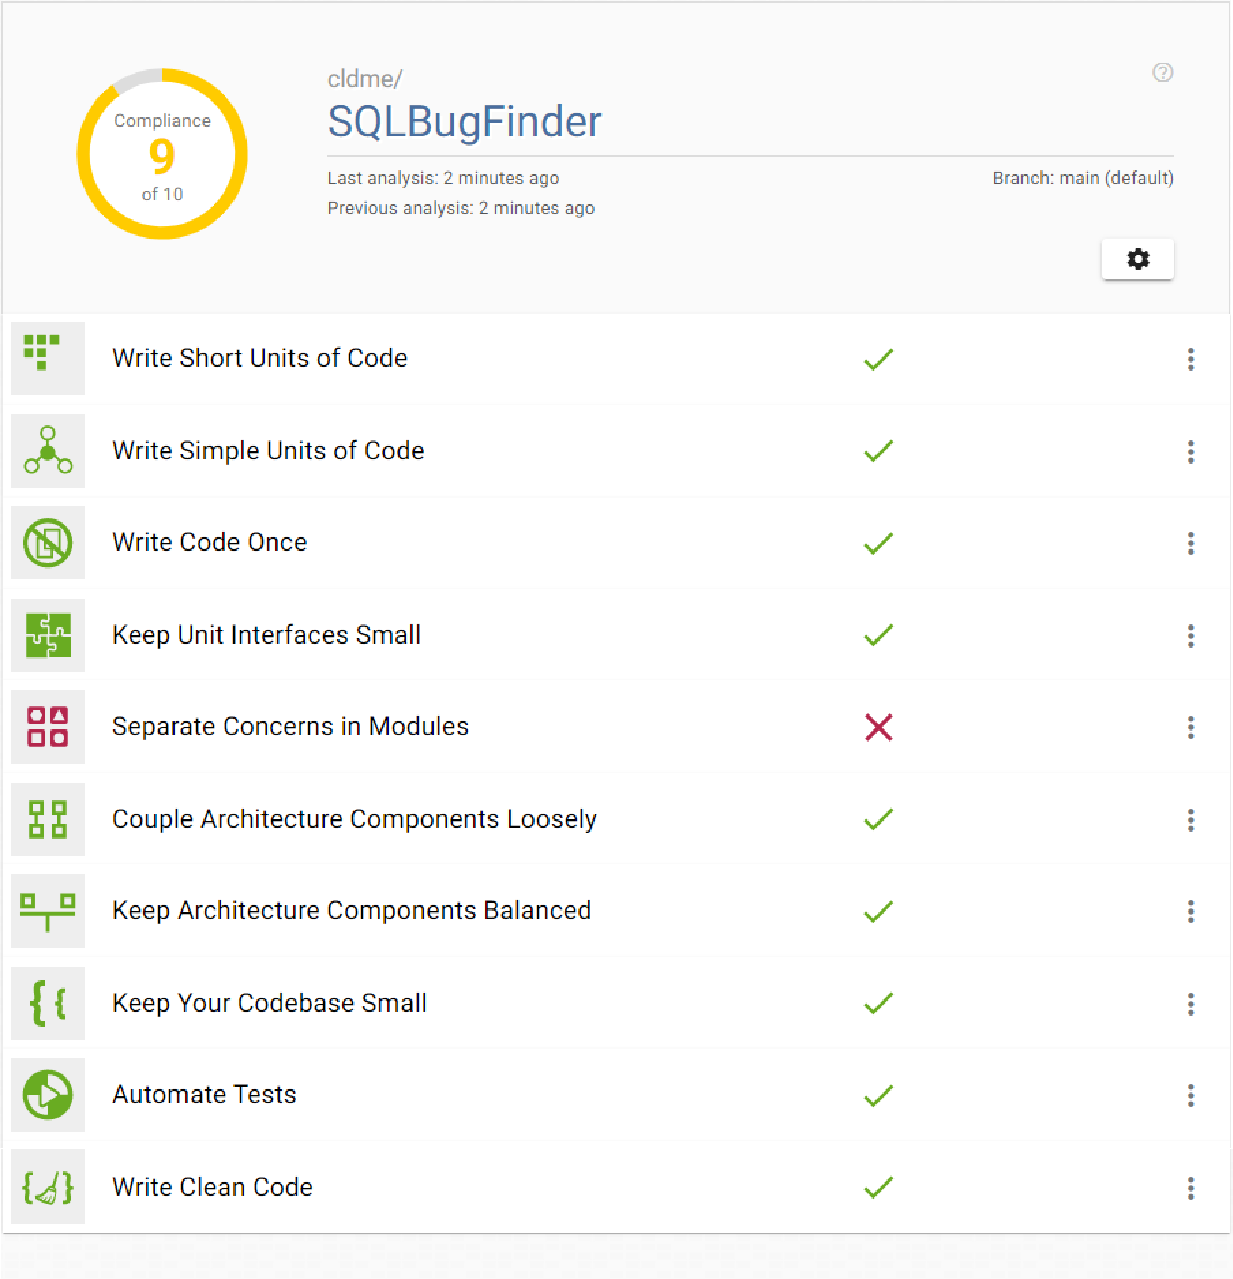
\includegraphics[width=0.95\textwidth]{img/code_hub.pdf}
    \caption{Code quality analysis}
    \label{fig:code_quality}
\end{figure}

\end{document}
